\chapter{Real Data from pp Collisions}
\label{ch:realdata}

\section{Primary Datasets}
The Run 2 of the LHC started in 2015 after a long shutdown of two years, colliding protons at a center-of-mass energy of 13 TeV. After resuming operations, the CMS experiment collected proton-proton collision data equivalent to an integrated luminosity of 3.8 fb$^{-1}$. The fraction of certified data with good magnetic field and without HF --- Hadronic Forward detector --- was 2.7 fb$^{-1}$. %; including the HF, the certified luminosity reduces to 2.3 fb$^{-1}$. 
Our analysis only uses central objects in the range $|\eta|<2.5$, then we are allowed to use the whole set of certified data.%, {\it i.e.} 2.7 fb$^{-1}$ of integrated luminosity.

We would like to remind the problems faced by the cryogenic system of the CMS magnet which restricted the amount of data collected with the standard 3.8~T field configuration. Despite those unexpected developments, we did our best to incorporate in this thesis the 2016 data but those efforts did not converge in time and, therefore, only results obtained with the 2015 data were included.

CMS primary datasets, the Analysis Object Data (AOD) files, contains the necessary information for the offline analysis. In 2015 a new format called MiniAOD \cite{miniAODtwiki} was created, which includes the following information:
\begin{compact_itemize}
\item High-level physics objects such as muons, electrons, photons, taus, jets, missing energy;
\item Monte Carlo information for simulated samples;
\item Primary vertex collection;
\item Trigger decision bits.
\end{compact_itemize}

A feature of the MiniAOD format is the absence of the track collection, which was dropped purposely in order to keep a small event size. Table \ref{tab:Datasets} contains the name of the datasets used in this analysis.  SingleElectron (SingleMuon) corresponds to the dataset filled with a stream of data triggered by electron (muon) objects. The second part of the name refers to the era (Run2015 C, D), the separation between bunches (25 ns), and the date of the reconstruction campaign (16Dec2015). The other columns in the table contain the integrated luminosity as well as the number of events. The specific version of the CMS software deployed during the data taken was 7\_4\_8\_patch1 for Run2015 C, and 7\_4\_15 for Run2015 D. The last re-reconstruction happened in December 2015, using CMS software version 7\_6\_3.

\begin{table}[htbp]
%\footnotesize
\centering
\caption{Description of the real data samples.}
\begin{tabular}{lcc}
&&\\
\textbf{Dataset Name}   & \textbf{\lumi \; (\pbinv)} & \textbf{Events}\\
\hline\hline
& \\
/SingleElectron/Run2015C\_25ns-16Dec2015     &  17.7       & 837 k       \\[0.3 cm]
/SingleElectron/Run2015D-16Dec2015           &   2672.8    & 134 M      \\
& \\
\hline
& \\
/SingleMuon/Run2015C\_25ns-16Dec2015       &    17.7     & 1.34 M         \\[0.3 cm]
/SingleMuon/Run2015D-16Dec2015            &   2672.8     & 92 M     \\
& \\
\hline
\end{tabular}
\label{tab:Datasets}
\end{table}

Events are recorded by the online selection algorithm requiring a single electron or a single muon. A triggering electron must have $p_{\rm T}>105$ GeV, while a triggering muon must have $p_{\rm T}>45$ GeV and $|\eta|<2.1$. We should recall that the trigger is also simulated in Monte Carlo samples as was discussed in the previous chapter. 

\begin{figure}[htb]
\centering
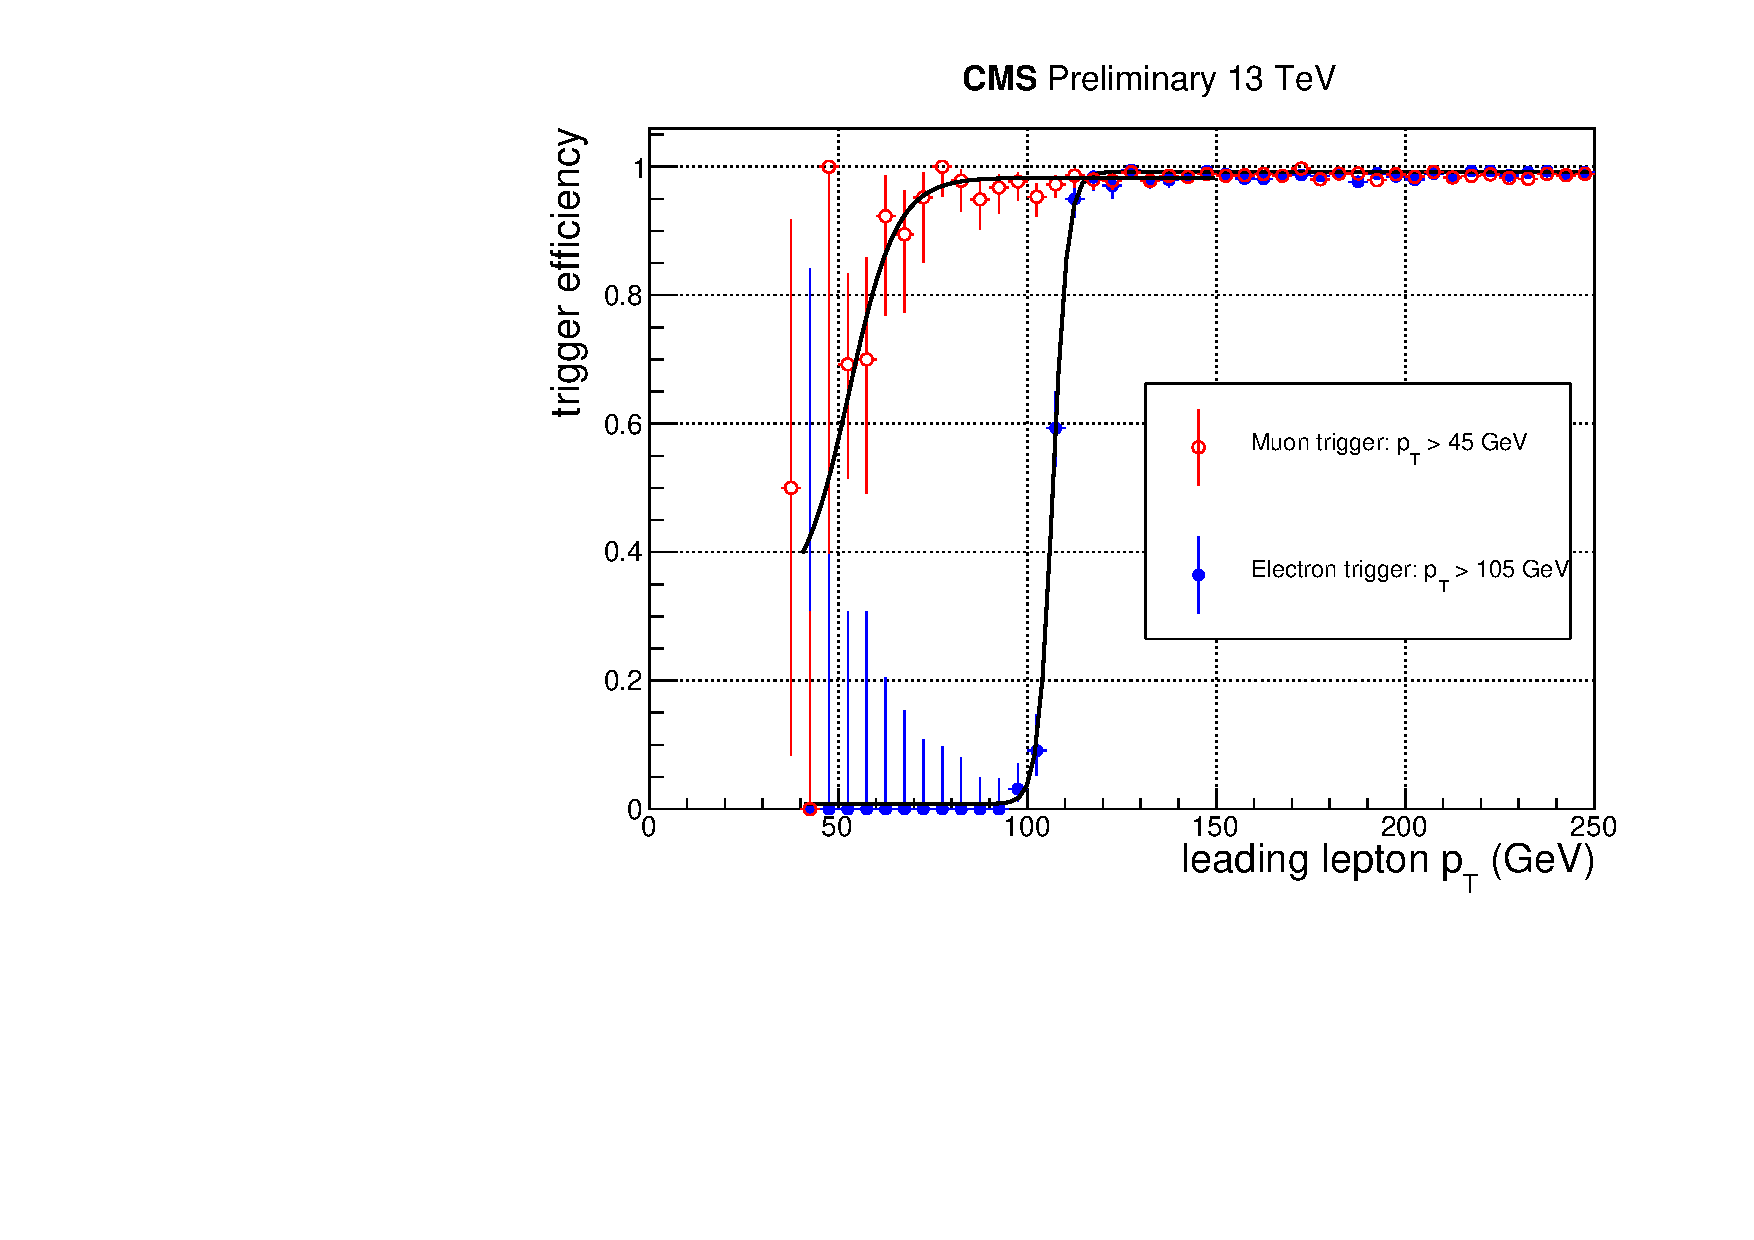
\includegraphics[width=0.85\textwidth]{figures/objects/trigger-eff-pt-lep1.pdf}
\caption[Trigger efficiency]{Simulation of the trigger efficiency as function of the leading lepton \ptrans.}
\label{fig:trigger}
\end{figure}

The performance of the trigger is analyzed by observing the turn-on curve shown in Fig. \ref{fig:trigger}. The numerator in the efficiency calculation corresponds to events passing the trigger, and the denominator includes the full event sample. The turn-on curve is modeled with a sigmoid function because the variable in the x-axis is the offline \ptrans rather than the online \ptrans; if the offline \ptrans were exactly the same as the online \ptrans, the trigger turn-on would be a step function. 

By convenience, the offline selection is chosen to accept events in the plateau of the trigger, which is the kinematic region where the efficiency is practically 100\%. The simulated samples are corrected for observed differences with the real data concerning trigger efficiencies; those trigger scale factors are close to unity, and the impact of this correction is accounted in the final result as a systematic uncertainty.

\section{Kinematic Distributions in the Control Region}
According to the analysis strategy established in the previous chapter,  we initially split the data into signal and control regions with the aim of blinding the signal and restricting the offline analysis to the control regions. For this reason, the remaining part of this chapter will contain distributions excluding the signal region.  

The offline analysis starts by selecting events with at least one reconstructed collision vertex within the distance of 24~cm along the beam axis and 2~cm in the transverse plane to the beams from the nominal pp interaction point. The vertex requirement is standard in CMS analyses \cite{Chatrchyan:2014fea}, and it is fundamental to identify high level objects. For instance, the identification of charged leptons involves a requirement on the impact parameter between the lepton's track and the primary vertex, in order to veto leptons from cosmic rays.

The number of primary vertices per event is a wide distribution with mean value $\sim$~10, as shown in Fig. \ref{nVtx_VZ}. We may recall that in Monte Carlo (MC) samples the pileup is simulated by superimposing minimum bias events on top of the hard process; the inaccuracy of the pileup simulation is therefore compensated with a reweighting procedure. The pileup weights are obtained by dividing the distribution of the true number of interactions in data and MC, and then, these weights are applied to the MC distributions.

In Fig. \ref{nVtx_VZ}, four categories are shown: 
\begin{compact_itemize}
\item muon low purity (top-left);
\item electron low purity (top-right);
\item muon high purity (bottom-left);
\item electron high purity (bottom-right).
\end{compact_itemize}

The MC distribution is a stacked histogram with different background components, namely, Z+jets, diboson, and $t\bar{t}$; the statistical uncertainty due to the limited amount of simulated events is also displayed. From the figure, we observe that Z+jets is the dominant component with a contribution larger than 95\%, while the remaining backgrounds --- diboson and $t\bar{t}$ --- correspond to the subdominant component. Moreover, the real data in the figure correspond to the points with the associated error bars. Additionally, the small panel below every distribution contains the Data/MC ratio, which is summarized in the Table \ref{dataMCratio}. 

\vspace{1cm}
\begin{table}[h!]
\begin{center}
\caption[Data/MC ratios]{Events yields and Data/MC ratios in the control region.}
\label{dataMCratio}
\begin{tabular}{lccc}
\hline
&&&\\[-0.2cm]
\textbf{Category}    & \textbf{Data} & \textbf{MC}   &\textbf{Data/MC} \\[0.2cm]
 \hline\hline
 &&&\\[-0.2cm]
Muon Low Purity      & 398           & 440           & 0.90 \\[0.2cm]
Muon High Purity     &  68           & 67            & 1.01 \\[0.2cm]
Electron Low Purity  & 271           & 335           & 0.81 \\[0.2cm]
Electron High Purity &  44           & 53            & 0.82 \\[0.2cm]
\hline
\end{tabular}
\end{center}
\end{table}

\begin{figure}[h]
\begin{center}
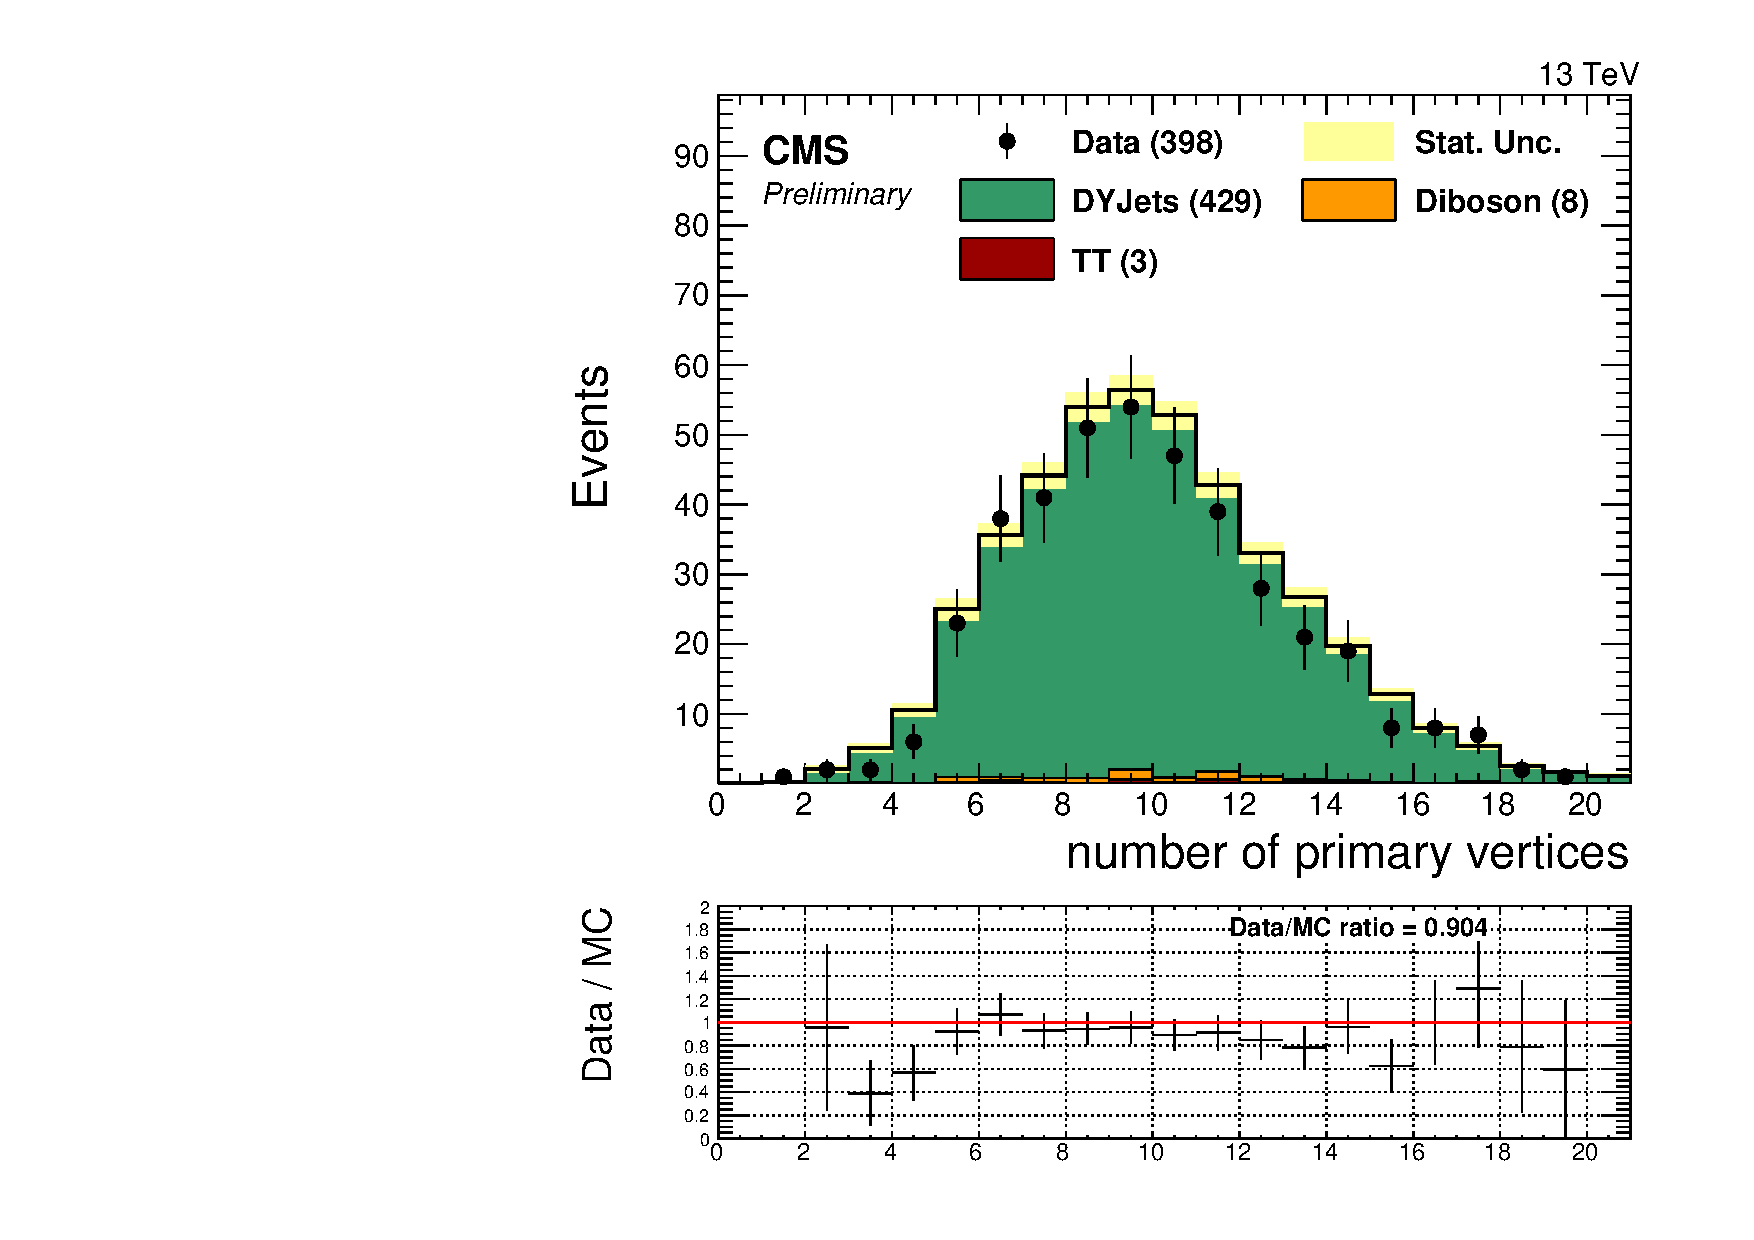
\includegraphics[scale=0.37]{figures/control/nVtxMLP.pdf}
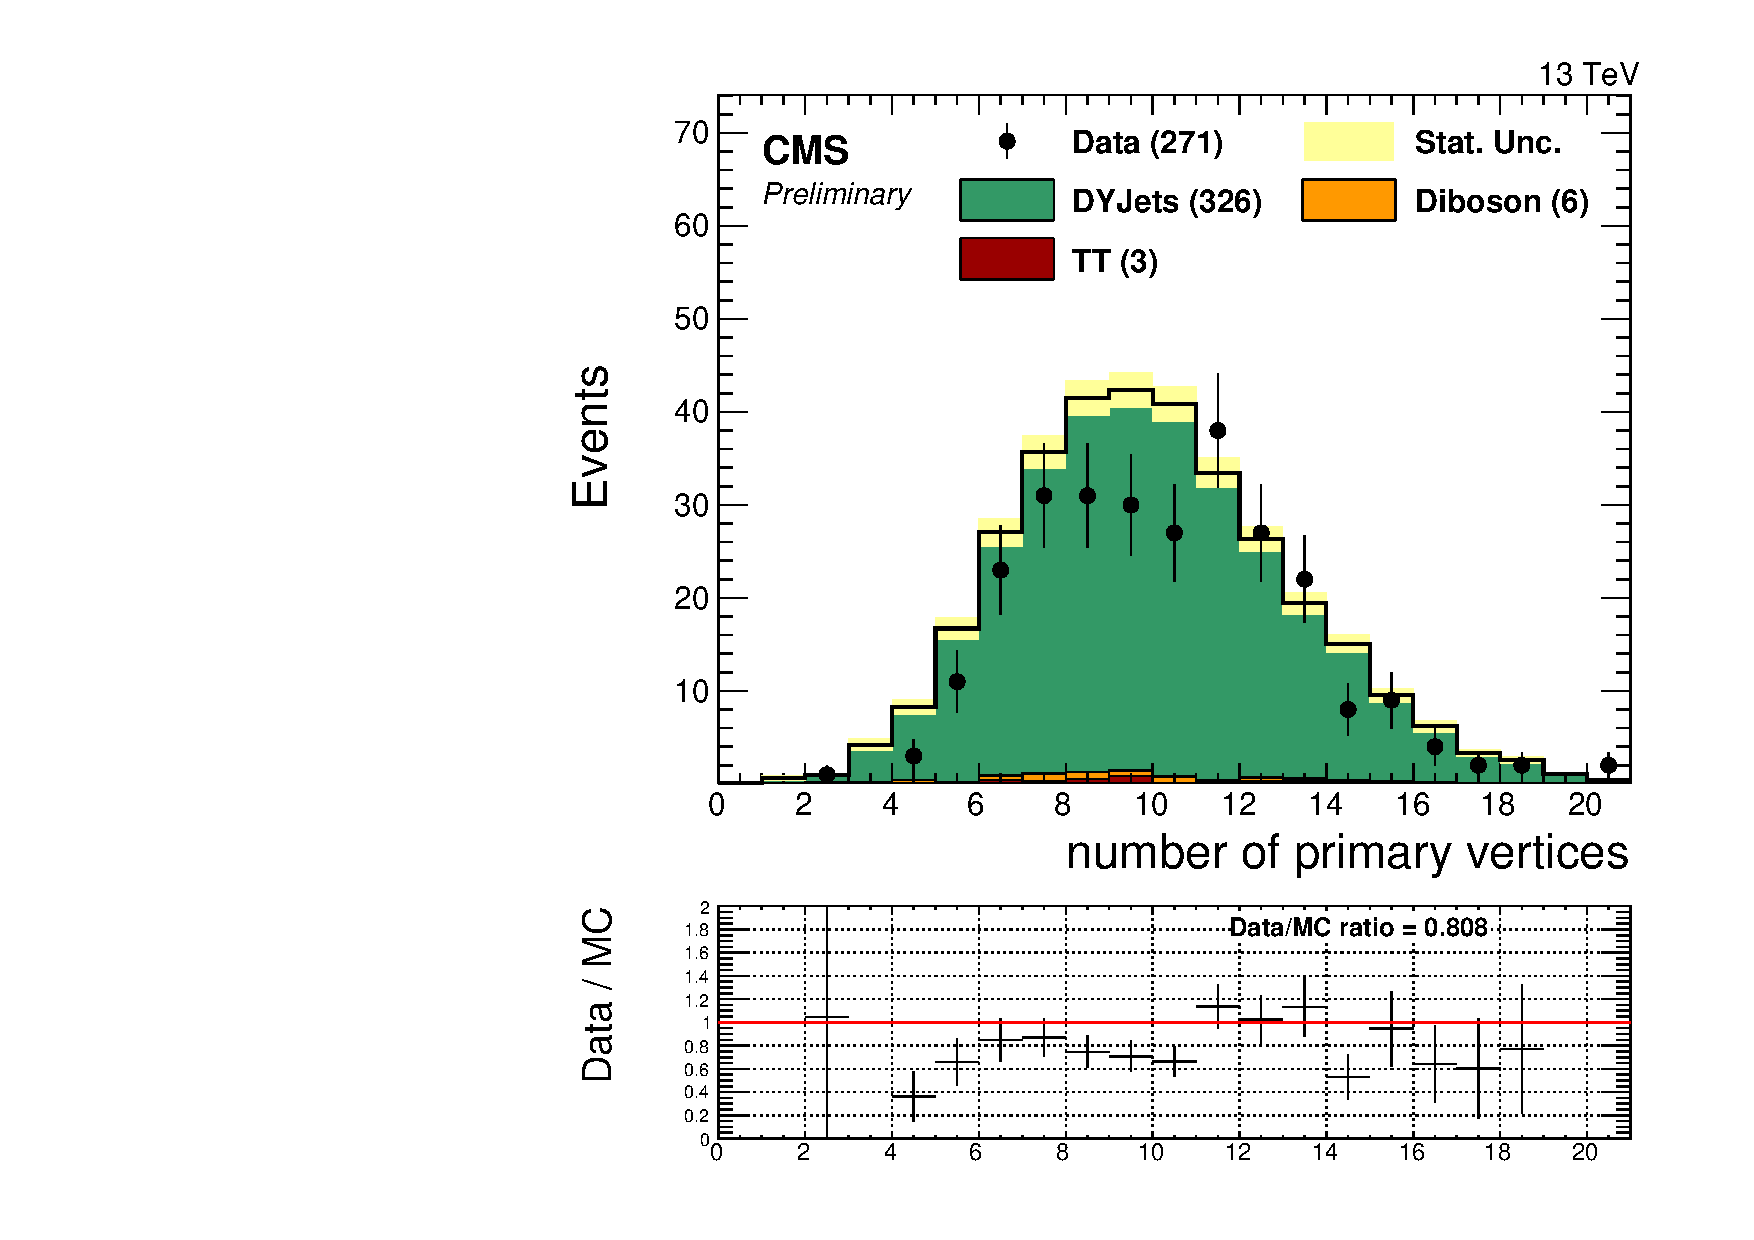
\includegraphics[scale=0.37]{figures/control/nVtxELP.pdf}\\ [2cm]
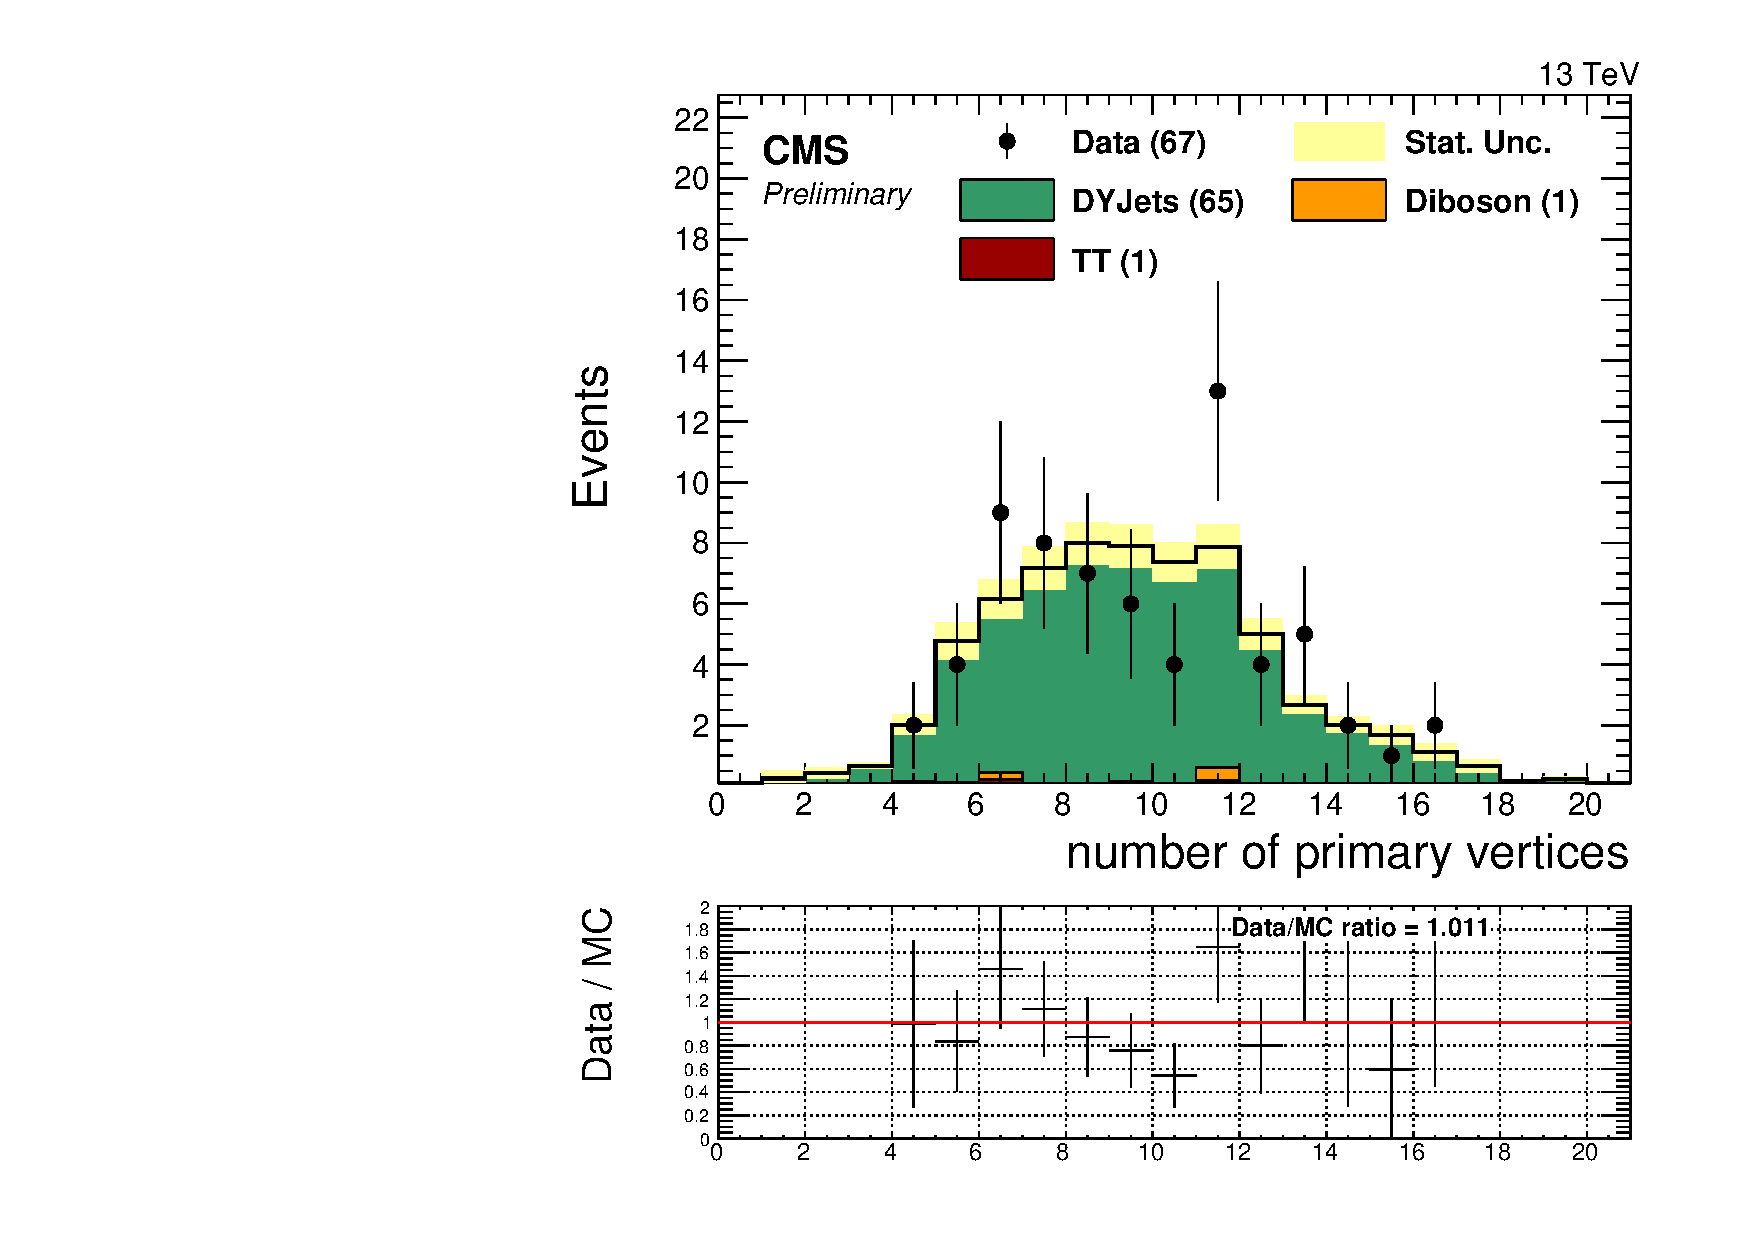
\includegraphics[scale=0.37]{figures/control/nVtxMHP.pdf}
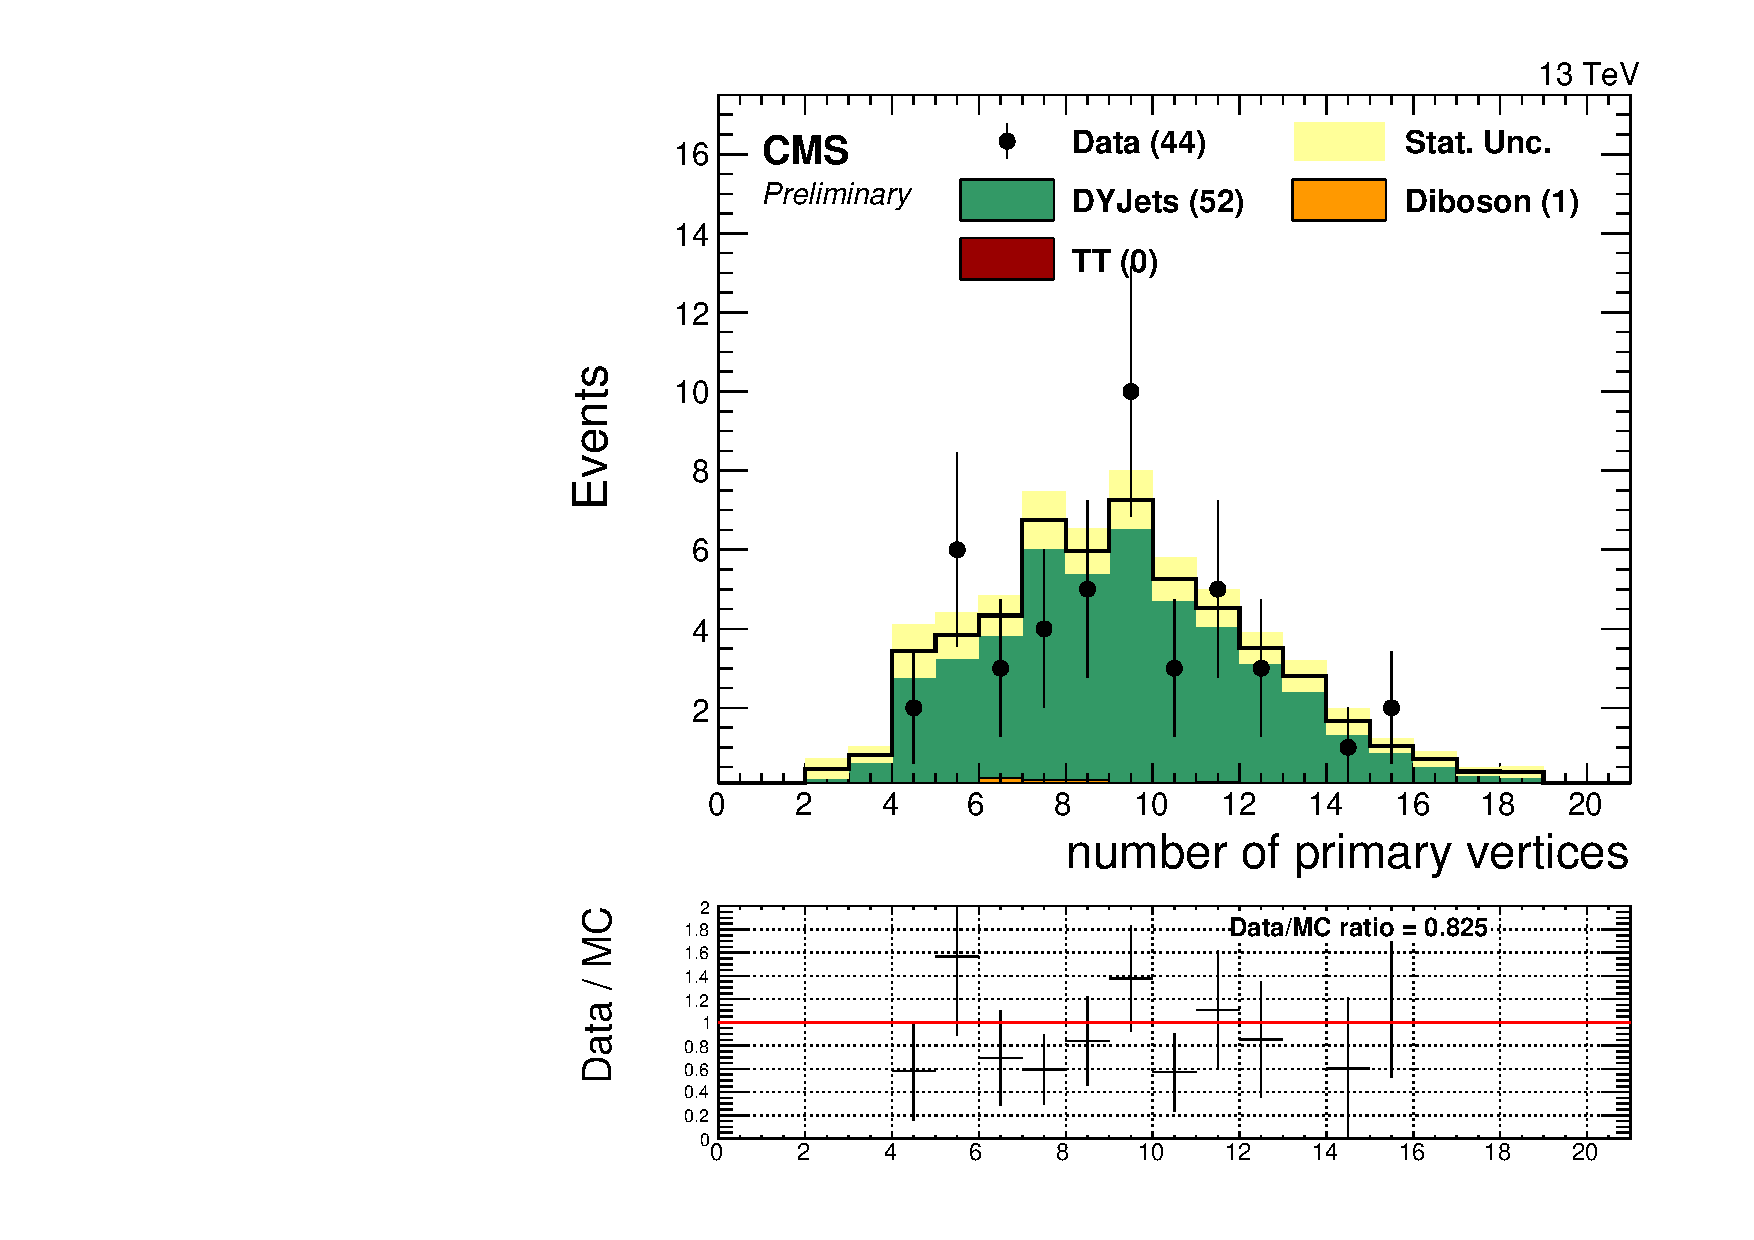
\includegraphics[scale=0.37]{figures/control/nVtxEHP.pdf}
\caption[Distribution of number of primary vertices]{Distribution of number of primary vertices.  Four categories are shown: muon low purity (top-left), electron low purity (top-right), muon high purity (bottom-left), and electron high purity (bottom-right).}
\label{nVtx_VZ}
\end{center}
\end{figure}

\clearpage
\subsection{Leptonic Z Selection}

Leptonic Z candidates are selected from a pair of same-flavour and opposite-charge leptons $\ell^+\ell^-$, where $\ell = e, \mu$. The analysis distinguishes electron and muon categories: Z candidates formed by electrons (muons) belong to the electron (muon) channel. Leptons originated from the decay of high \ptrans bosons are expected to be closer to each other with small $\Delta R(\ell^+ \ell^-)$. In this boosted regime, one lepton may spoil the isolation of the other due to the coarse detector resolution in the muon chambers and the calorimeters. For smaller values of $\Delta R(\ell^+ \ell^-)$ a drop in efficiency may occur, unless we apply dedicated identification and isolation requirements. The identification criteria for electrons and muons that optimize the efficiency in the boosted regime are described below.

\subsection*{Electron Identification}
The electron identification is chosen from the recommendations of the EGamma physics object group \cite{egammaPOG}. We use particle-flow electron candidates with loose requirements defined below:

\begin{compact_itemize}
\item Pseudo rapidity $|\eta|$ of the electron's supercluster: $ < 1.479$ (Barrel), and between $1.479$ and $2.5$ (Endcap);
\item Difference in $\eta$ between the track position as measured in the inner layer, extrapolated to the interaction vertex and then extrapolated to the calorimeter and the $\eta$ of the seed cluster of the supercluster $<$ 0.0095 (Barrel), 0.010 (Endcap);
\item Difference in $\phi$ between the track position as measured in the inner layer, extrapolated to the interaction vertex and then extrapolated to the calorimeter and the $\phi$ of the seed cluster of the supercluster $<$ 0.18 (Barrel), 0.11 (Endcap);
\item Hadronic energy over electromagnetic energy $<$ 0.082 (Barrel), 0.10 (Endcap);
\item Relative isolation in a cone of aperture $R=0.3$ with effective area correction $<$ 0.118 (Barrel), 0.089 (Endcap);
\item Number of inner tracker layers lost hits $<$ 1 (Barrel), 2 (Endcap).
\end{compact_itemize}

The efficiency of this working point is evaluated in Fig. \ref{fig:eleid} using simulated samples of the bulk graviton signal. The mass of the graviton ranges between 0.8 to 2.5 TeV, and all mass points have been added to produce a result with good statistics. The efficiency is found to be around 84\% for $\Delta R$ separations between 0.15 and 0.5. We studied the impact of the isolation which is embedded by default in the electron identification working point, getting an efficiency around 90\% when the isolation is removed. For close-by electrons ($\Delta R < 0.08$) the efficiency drops to 65\%.

\begin{figure}[htb]
\centering
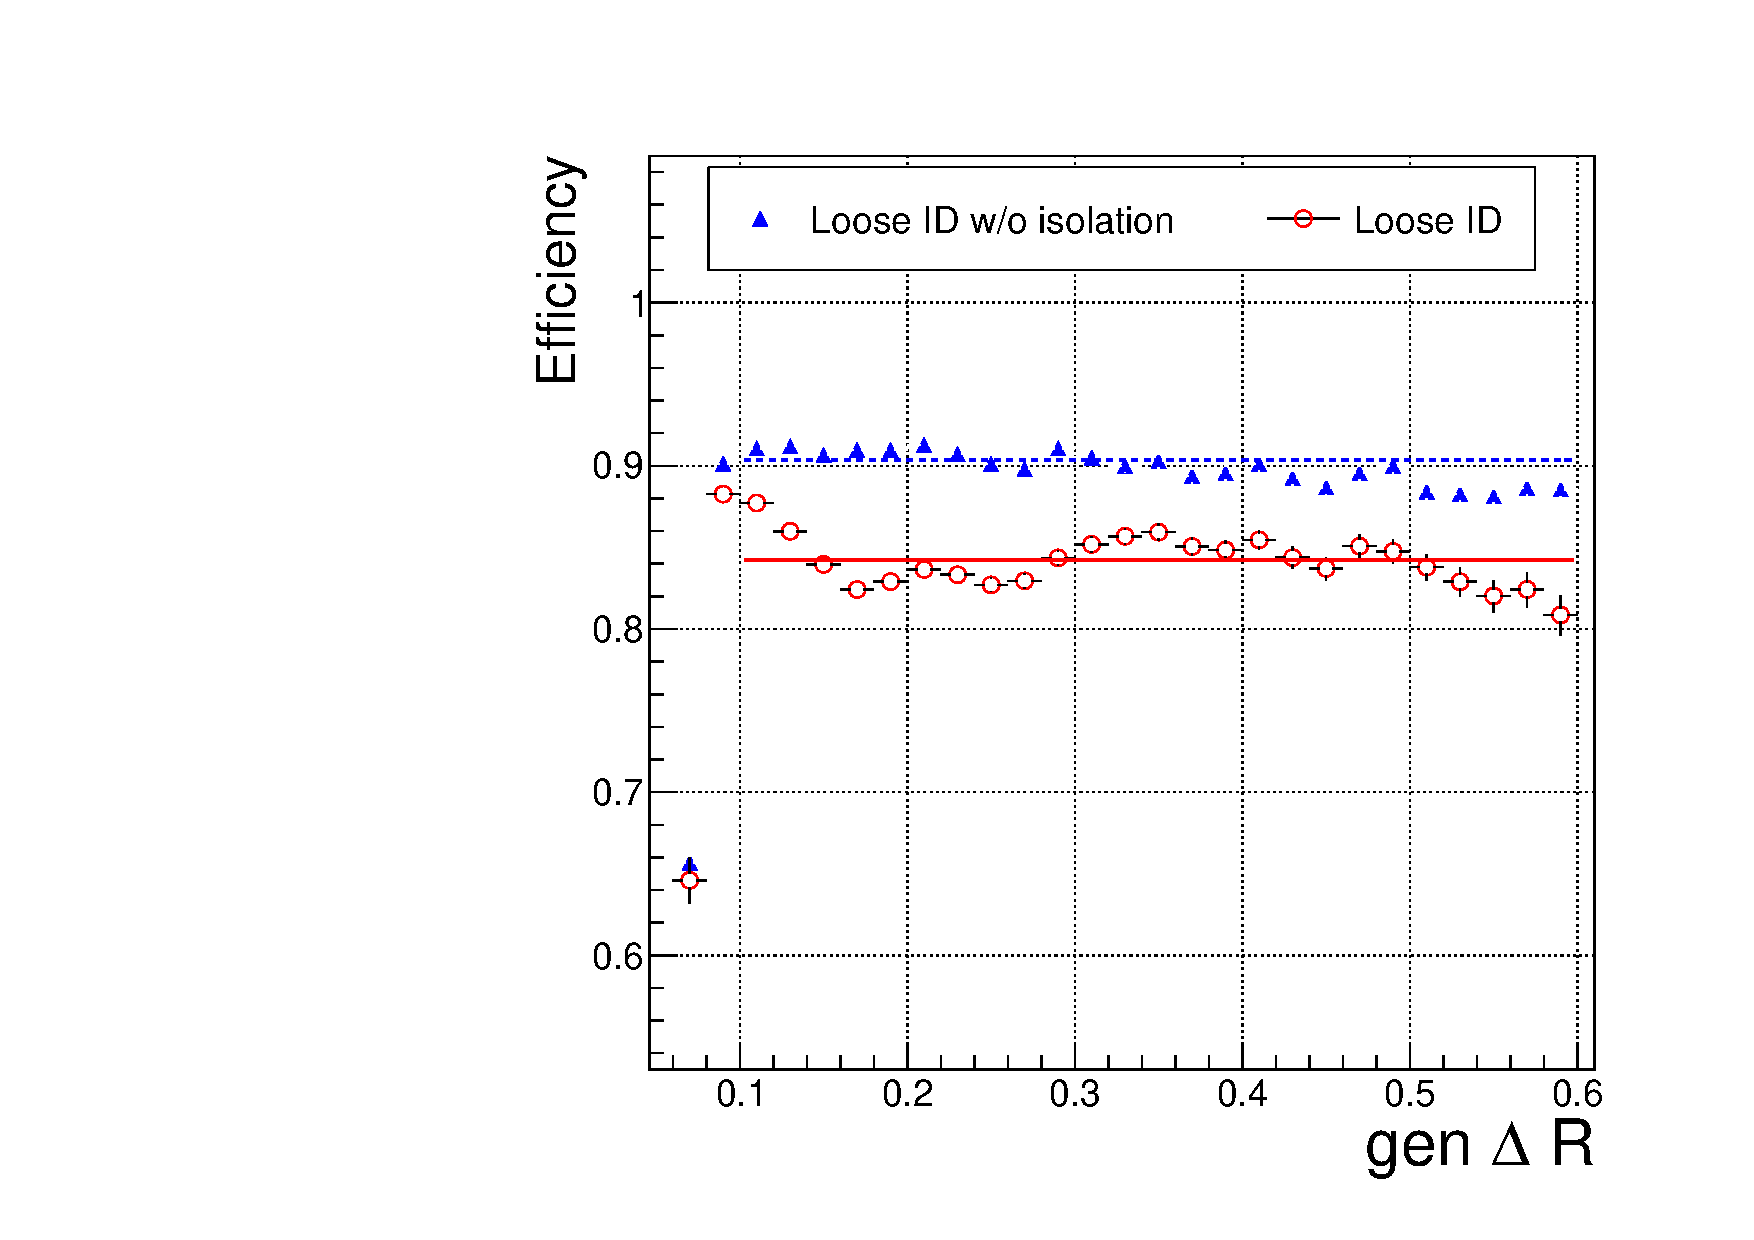
\includegraphics[width=0.7\textwidth]{figures/objects/id-eff-dR-ele.pdf}
\caption[Electron identification efficiency]{Electron identification efficiency for the loose working point (red open markers) as function of the $\Delta R$ separation between the electrons.} %In order to measure the impact of the isolation, the efficiency without isolation (blue markers) is also shown.}
\label{fig:eleid}
\end{figure}

On top of the identification working point we apply additional requirements such that the leading (subleading) electron satisfies \ptrans  $\geq 115 \, (50)$  GeV and $|\eta| < 2.4$; the pseudorapidity requirement ensures the electrons are inside the geometric acceptance of the detector. The \ptrans requirements in the offline selection are tighter than the online trigger, to avoid inefficiencies occurring at values lower than the trigger threshold.

Additionally, the Monte Carlo events are corrected with isolation and identification scale factors that improve the agreement with real data. The computation of the scale factors is done directly by the EGamma physics object group, and the systematic uncertainty associated with this correction was carefully evaluated in our analysis as will be explained in Section \ref{sec:systematics}.

\subsection*{Muon Identification}
The muon identification and their momentum assignment follow the recommendation of the muon physics object group \cite{muonPOG}. The high \ptrans working point is used for the leading candidate, specifically:
\begin{compact_itemize}
\item Muon identified as global muon;
\item At least one muon chamber hit included in the global-muon track fit;
\item Muon segments in at least two muon stations;
\item Tracker track transverse impact parameter $d_{xy} < 2$ mm;
\item Longitudinal impact parameter $d_z < 5$ mm;
\item Number of pixel hits larger than zero;
\item Number of tracker layers with hits $> 5$;
\item Muon track $dp_{\rm T} / p_{\rm T} < 0.3$.
\end{compact_itemize}

\begin{figure}[!h]
\centering
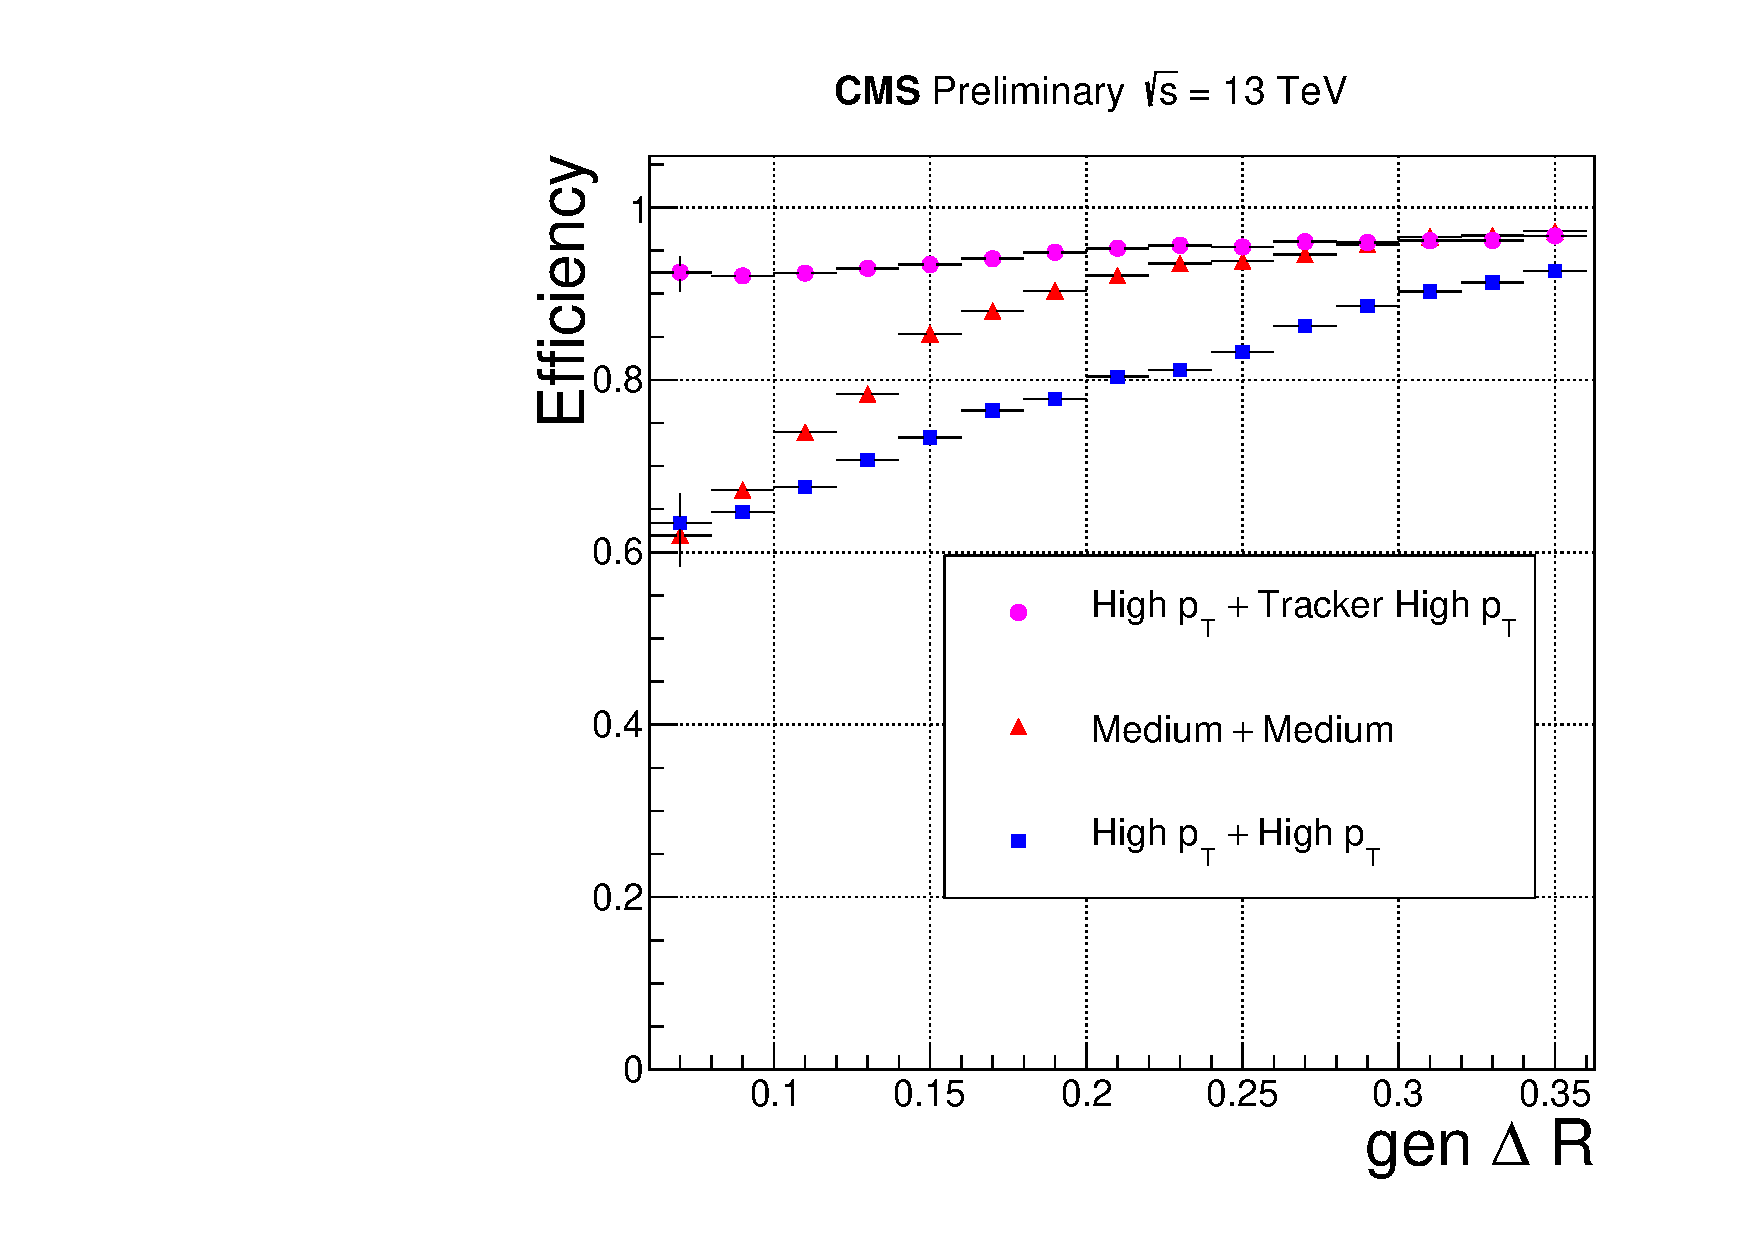
\includegraphics[width=0.6\textwidth]{figures/objects/id-eff-dR-mu.pdf}
\caption[Muon identification efficiency]{Muon identification efficiency as function of the $\Delta R$ separation. The tracker high \ptrans identification recovers the inefficiencies in the case of close-by muons.}
\label{fig:muid}
\end{figure}

The tracker high \ptrans is a customized working point used for the sub-leading muon. It was developed to overcome the inefficiencies observed in the case of close-by muons. The tracker high \ptrans is essentially the high \ptrans working point without the global muon requirement; instead a tracker muon is selected. Fig. \ref{fig:muid} shows the muon identification efficiency for the bulk graviton signal as function of the $\Delta R$ separation, comparing the performance of different working points.

On top of the identification working point, muon candidates are required to have relative tracker isolation less than 0.1. For close-by muons ($\Delta R < 0.3$) the \ptrans of the inner track of one muon is removed from the isolation cone of the other, to avoid efficiency drops in the boosted regime. Lastly, the leading (sub-leading) muon also satisfies \ptrans  $\geq 50 \, (20)$  GeV and $|\eta| < 2.1 \, (2.4)$, in order to avoid inefficiencies occurring at values lower than the trigger threshold.

\subsection*{Lepton Kinematics}

Distributions of the \ptrans for the leading and sub-leading lepton are shown in Fig. \ref{ptlep1_VZ} and \ref{ptlep2_VZ}, respectively. Similarly, distributions of $\eta$ for the leading and sub-leading lepton are shown in Fig. \ref{etalep1_VZ} and \ref{etalep2_VZ}, respectively.  

In addition to the lepton identification requirements, dilepton candidates must have specific values of invariant mass $m_{\ell\ell}$ and transverse momentum $p_{\rm T}^{\ell\ell}$. Namely, $p_{\rm T}^{\ell\ell} > 170$  GeV and $70 < m_{\ell\ell} < 110$ GeV. These requirements intend to select Z candidates in the boosted region of the phase space; when more than one candidate is found, the highest \ptrans candidate is chosen.

Distributions of \ptrans and mass of the leptonic Z candidate are shown in Fig. \ref{ptZll_VZ} and \ref{massZll_VZ}, respectively. Similarly, the $\Delta R$ separation between the daughters of the leptonic Z candidate is shown in Fig. \ref{deltaRleplep_VZ}. 

\subsection{Hadronic Jet Selection}
The recommendations from the JetMET physics object group \cite{jetmetPOG} regarding jet identification include the following requirements:
\begin{compact_itemize}
\item Neutral Hadron Fraction $<$ 0.99;
\item Electromagnetic (EM) Fraction $<$ 0.99;
\item Number of Constituents $>$ 1;
\item Charged Hadron Fraction $>$ 0;
\item Charged Multiplicity $>$ 0;
\end{compact_itemize}
The jet identification is a loose requirement intended to reduce calorimeter noise. More important is the acceptance selection \ptrans $>$ 200 GeV, and $|\eta|<2.4$. Besides the jet substructure techniques described in Sec. \ref{JetSection}, no further requirements are applied, {\it e.g.} b tagging \footnote{The combine secondary vertex for b tagging is usually applied in the low energy regime when the merged (AK8) jet can be resolved into two (AK4) jets.}.

Figures \ref{ptZjj_VZ} and \ref{etaZjj_VZ} show the distributions of jet \ptrans and jet $\eta$ respectively. The $\Delta R$ separation between the jet and the closest lepton is shown in \ref{dRlepjet_VZ}. Figure \ref{massZjj_VZ} shows the distributions of the jet mass containing the gap in the signal region. The n-subjettiness variable $\tau_{21}$ is shown in Fig. \ref{tau21_VZ}. Finally, the distribution of the diboson invariant mass is shown in Fig. \ref{fig:candMass_VZ}. We recall that these distributions are blind, and the yields displayed in the legend of the plots account only the number of events in the control region.

From the analysis of the control region we conclude that there are remarkable discrepancies between the real data and the Monte Carlo simulation, concerning the normalization and the shape of several kinematic distributions. In Chapter \ref{bkgEstimation}, we will try a data-driven technique to estimate the invariant mass in the signal region relying on a interpolation of the data from the control regions. The technique known as alpha method \cite{Mozer:2016wzi} will be introduced, and we will obtain final limits based on the results of the data-driven estimation rather than the Monte Carlo simulations.

\begin{figure}[h]
\begin{center}
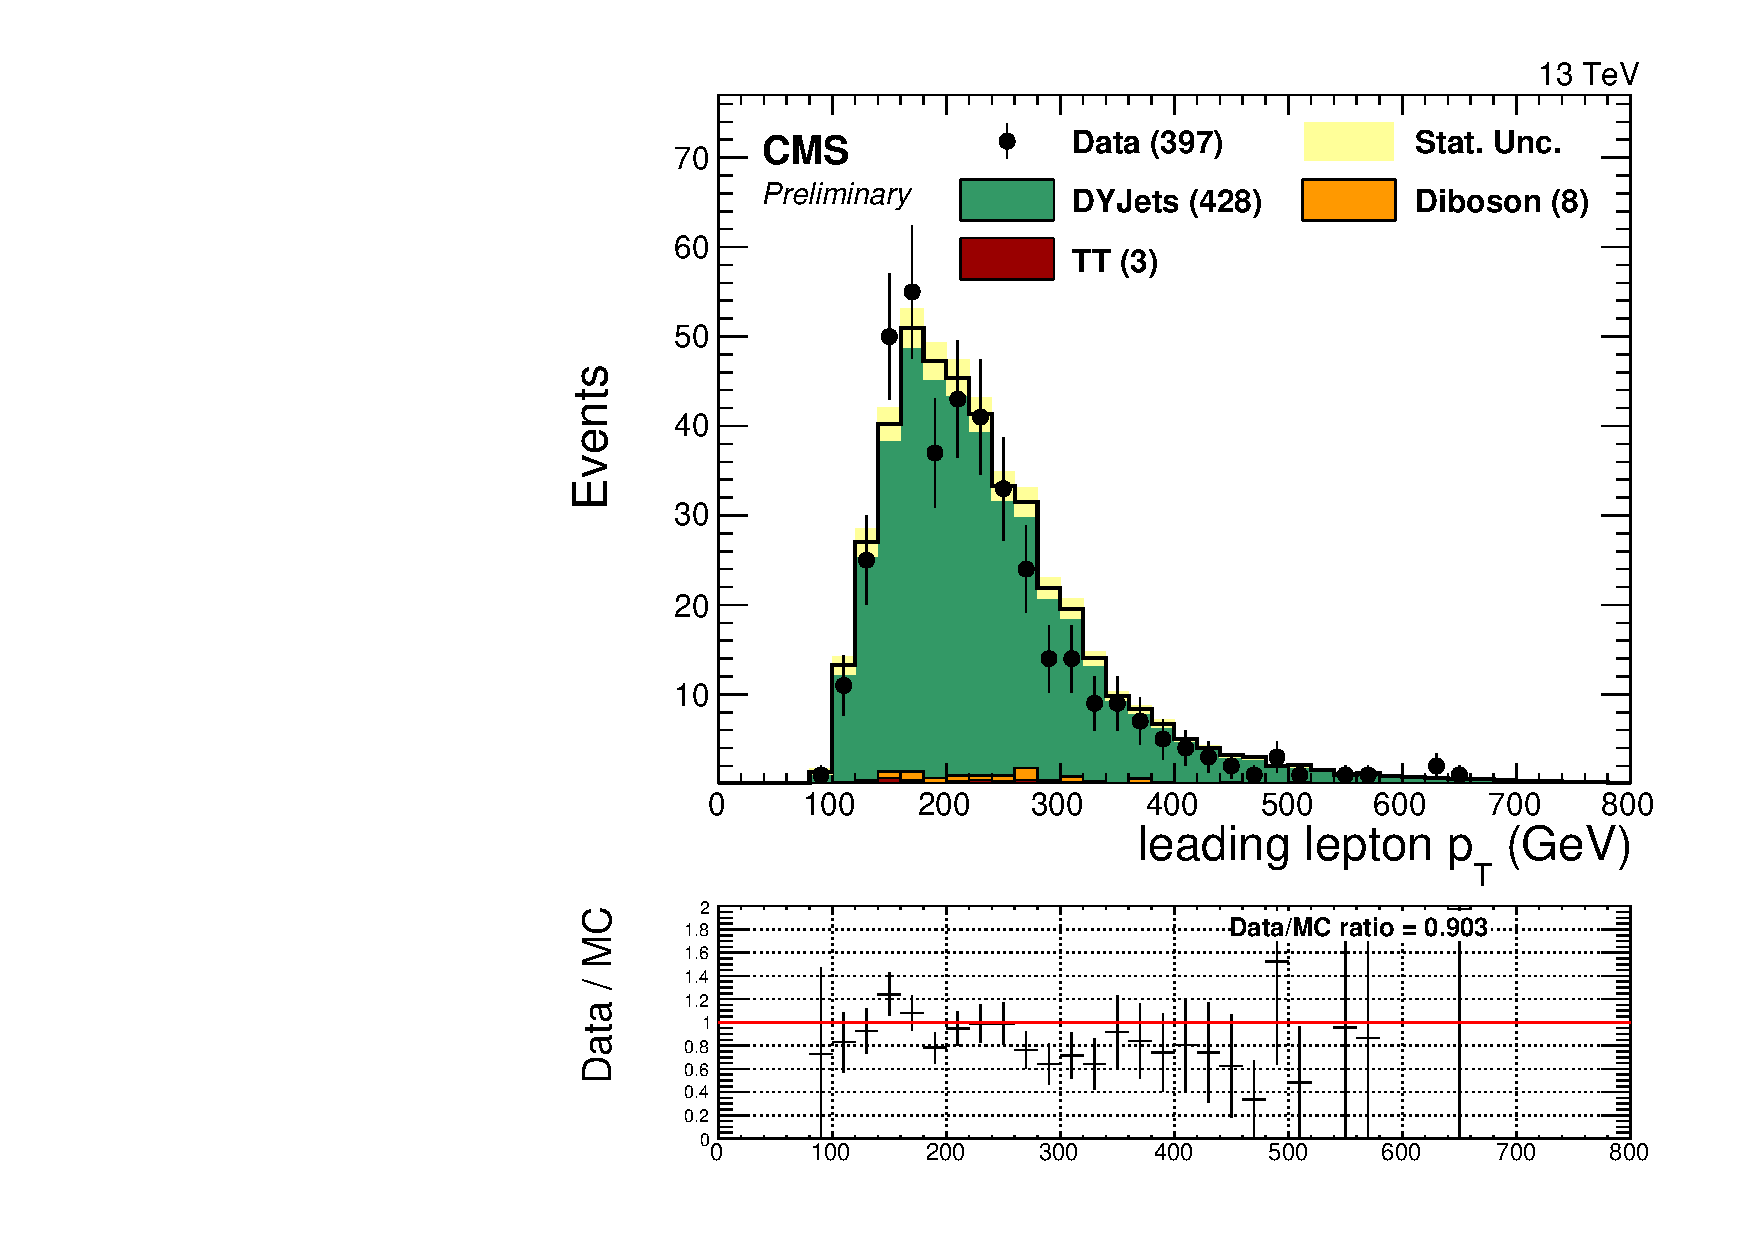
\includegraphics[scale=0.37]{figures/control/ptlep1MLP.pdf}
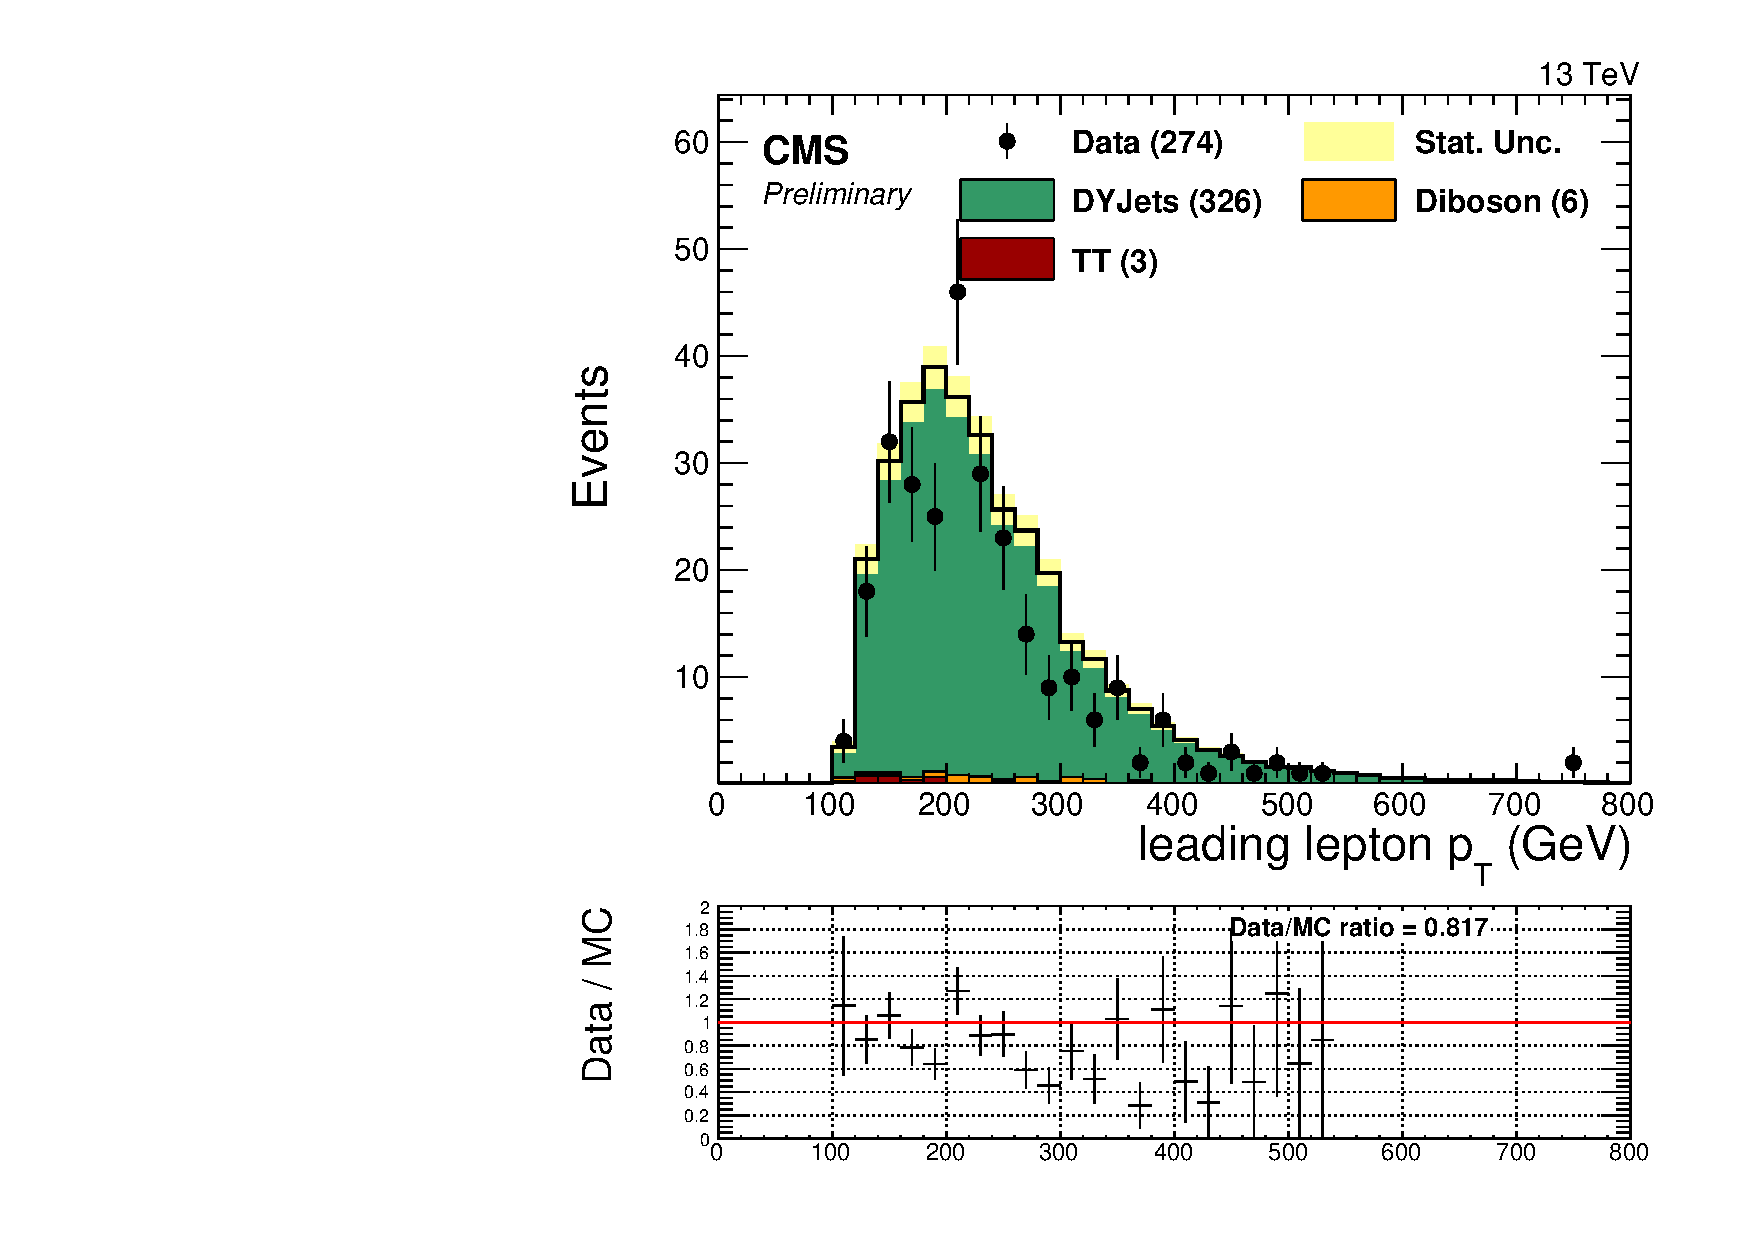
\includegraphics[scale=0.37]{figures/control/ptlep1ELP.pdf}\\[2cm]
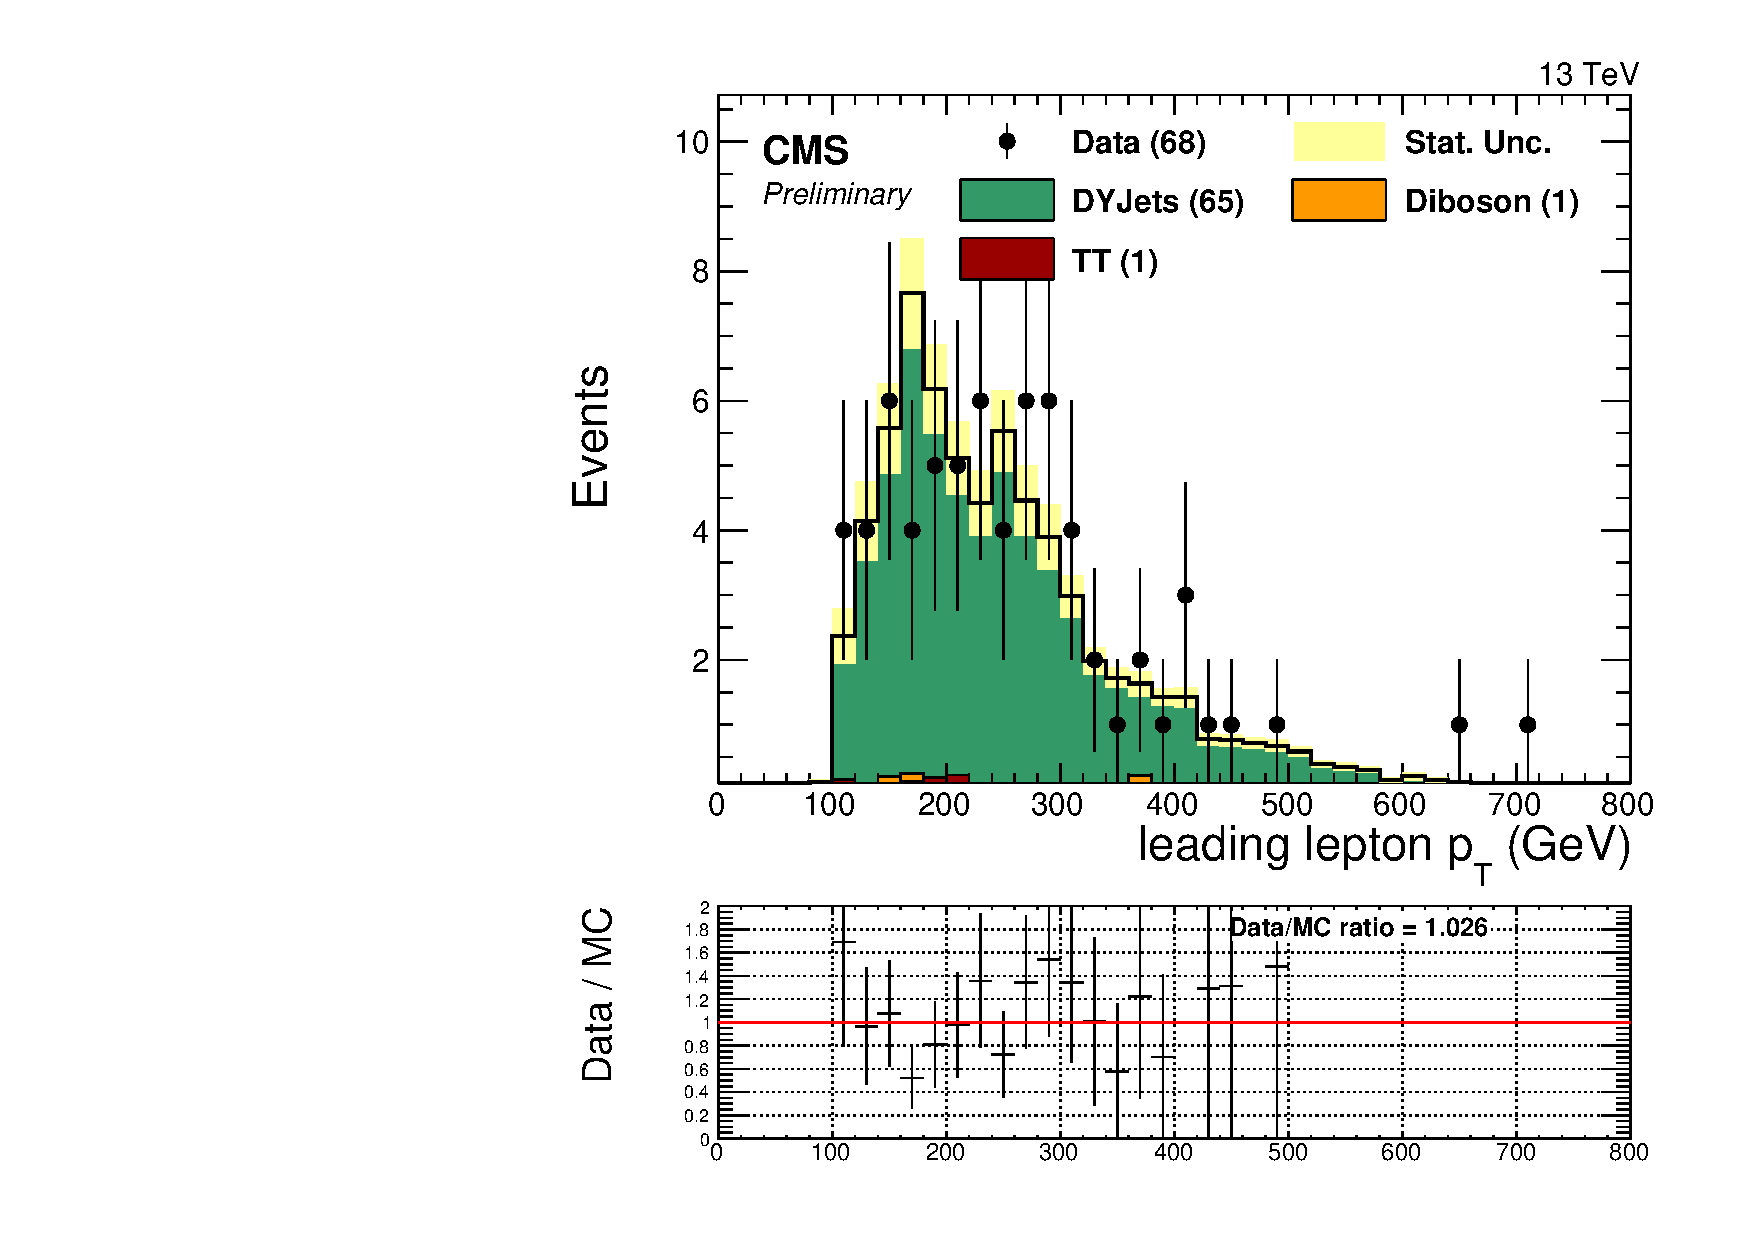
\includegraphics[scale=0.37]{figures/control/ptlep1MHP.pdf}
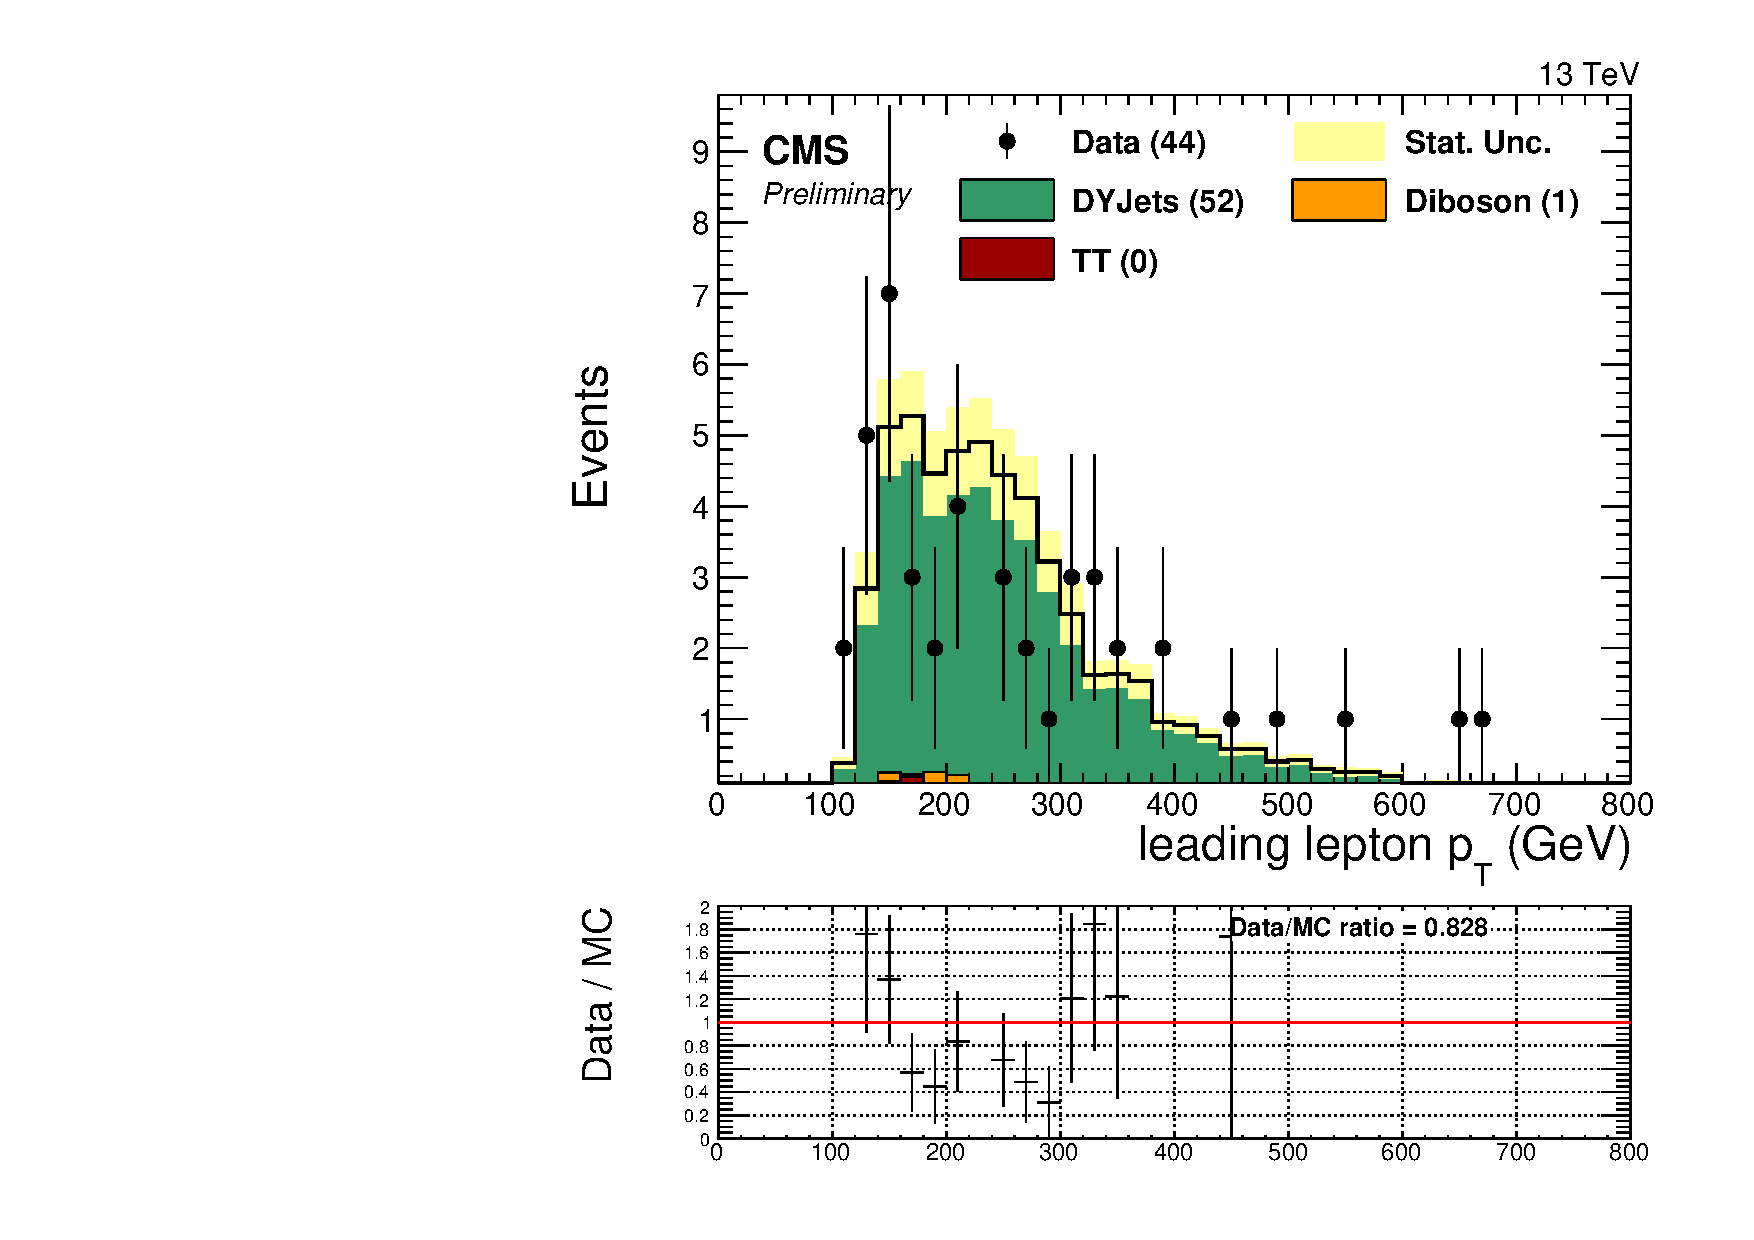
\includegraphics[scale=0.37]{figures/control/ptlep1EHP.pdf}
\caption[Distribution of \ptrans for the leading lepton]{Distribution of \ptrans for the leading lepton in the category: muon low purity (top-left), electron low purity (top-right), muon high purity (bottom-left), and  electron high purity (bottom-right). Simulated backgrounds are displayed as stacked histograms normalized to luminosity (2.7 fb$^{-1}$).}
\label{ptlep1_VZ}
\end{center}
\end{figure}
\begin{figure}[h]
\begin{center}
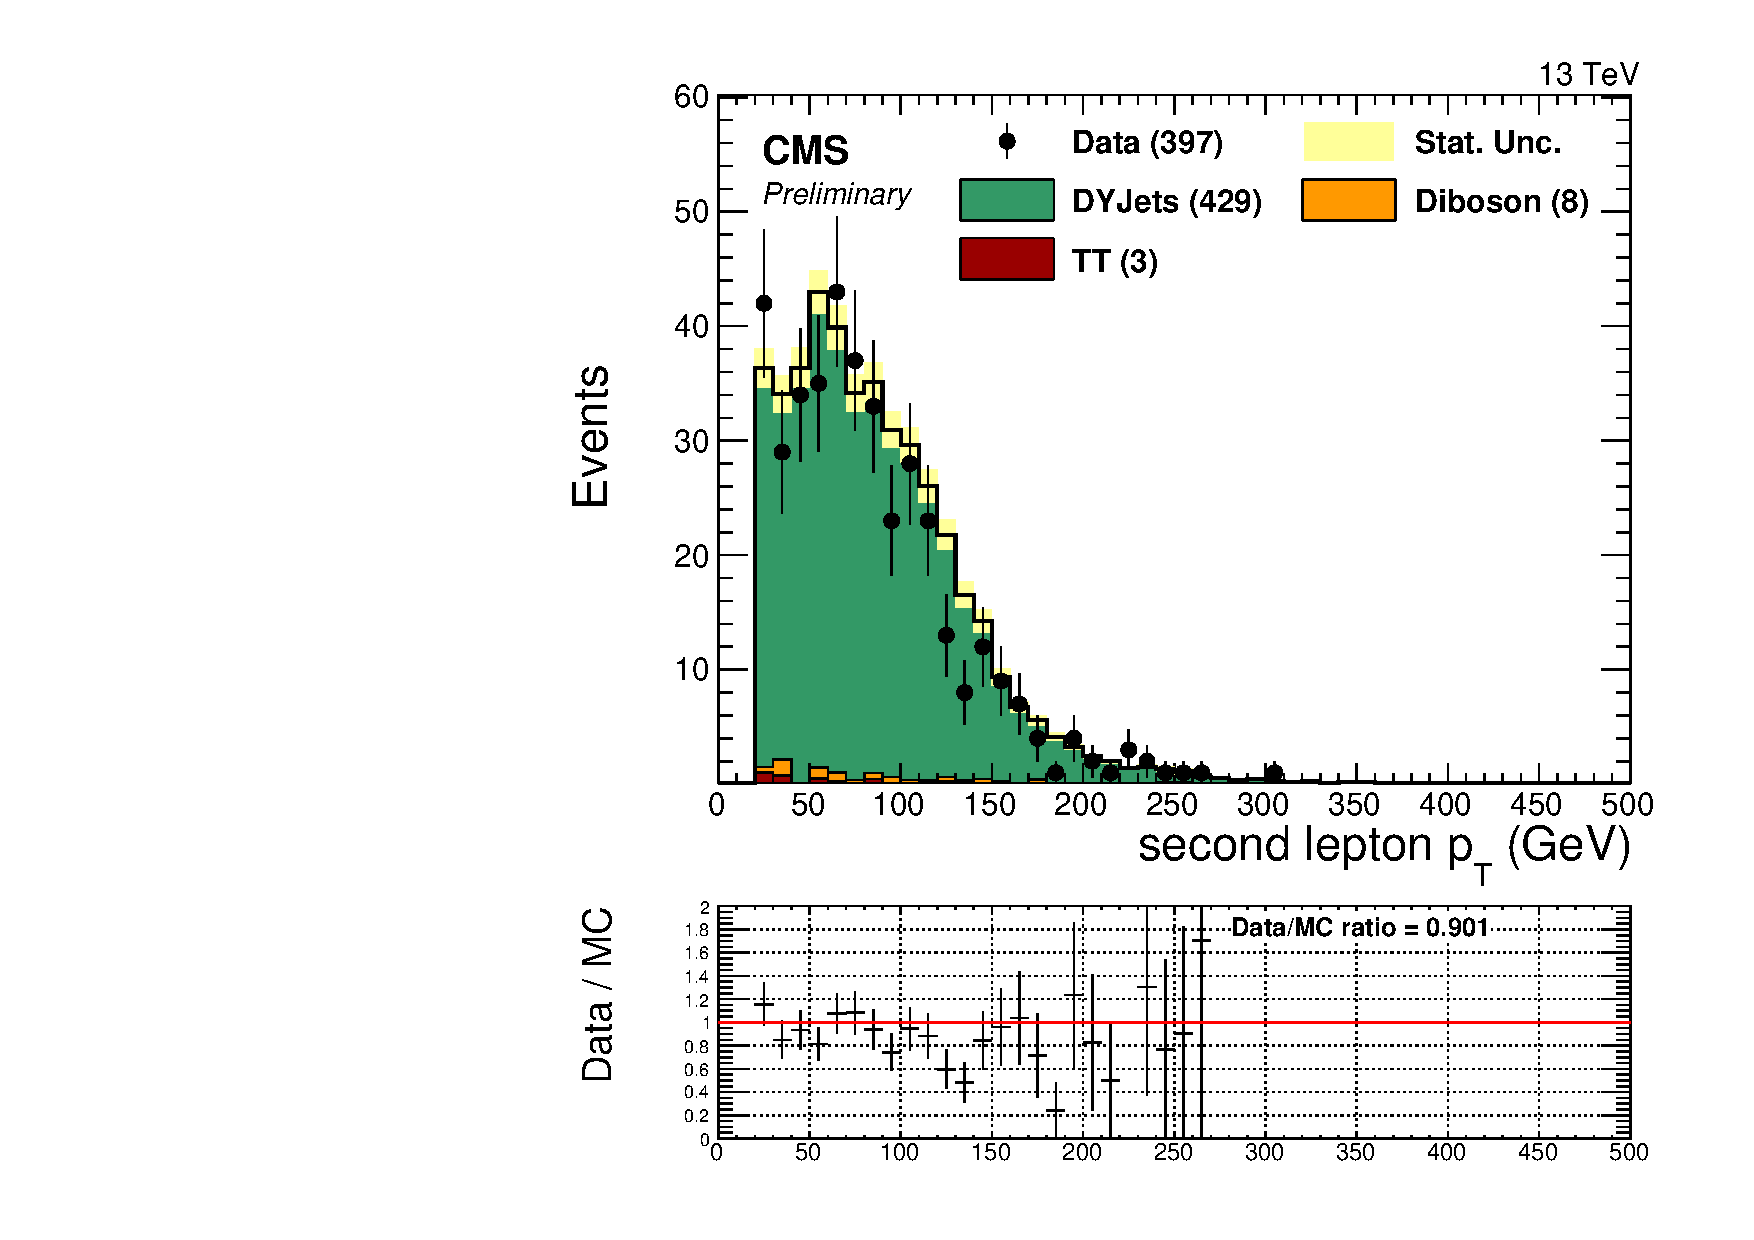
\includegraphics[scale=0.37]{figures/control/ptlep2MLP.pdf}
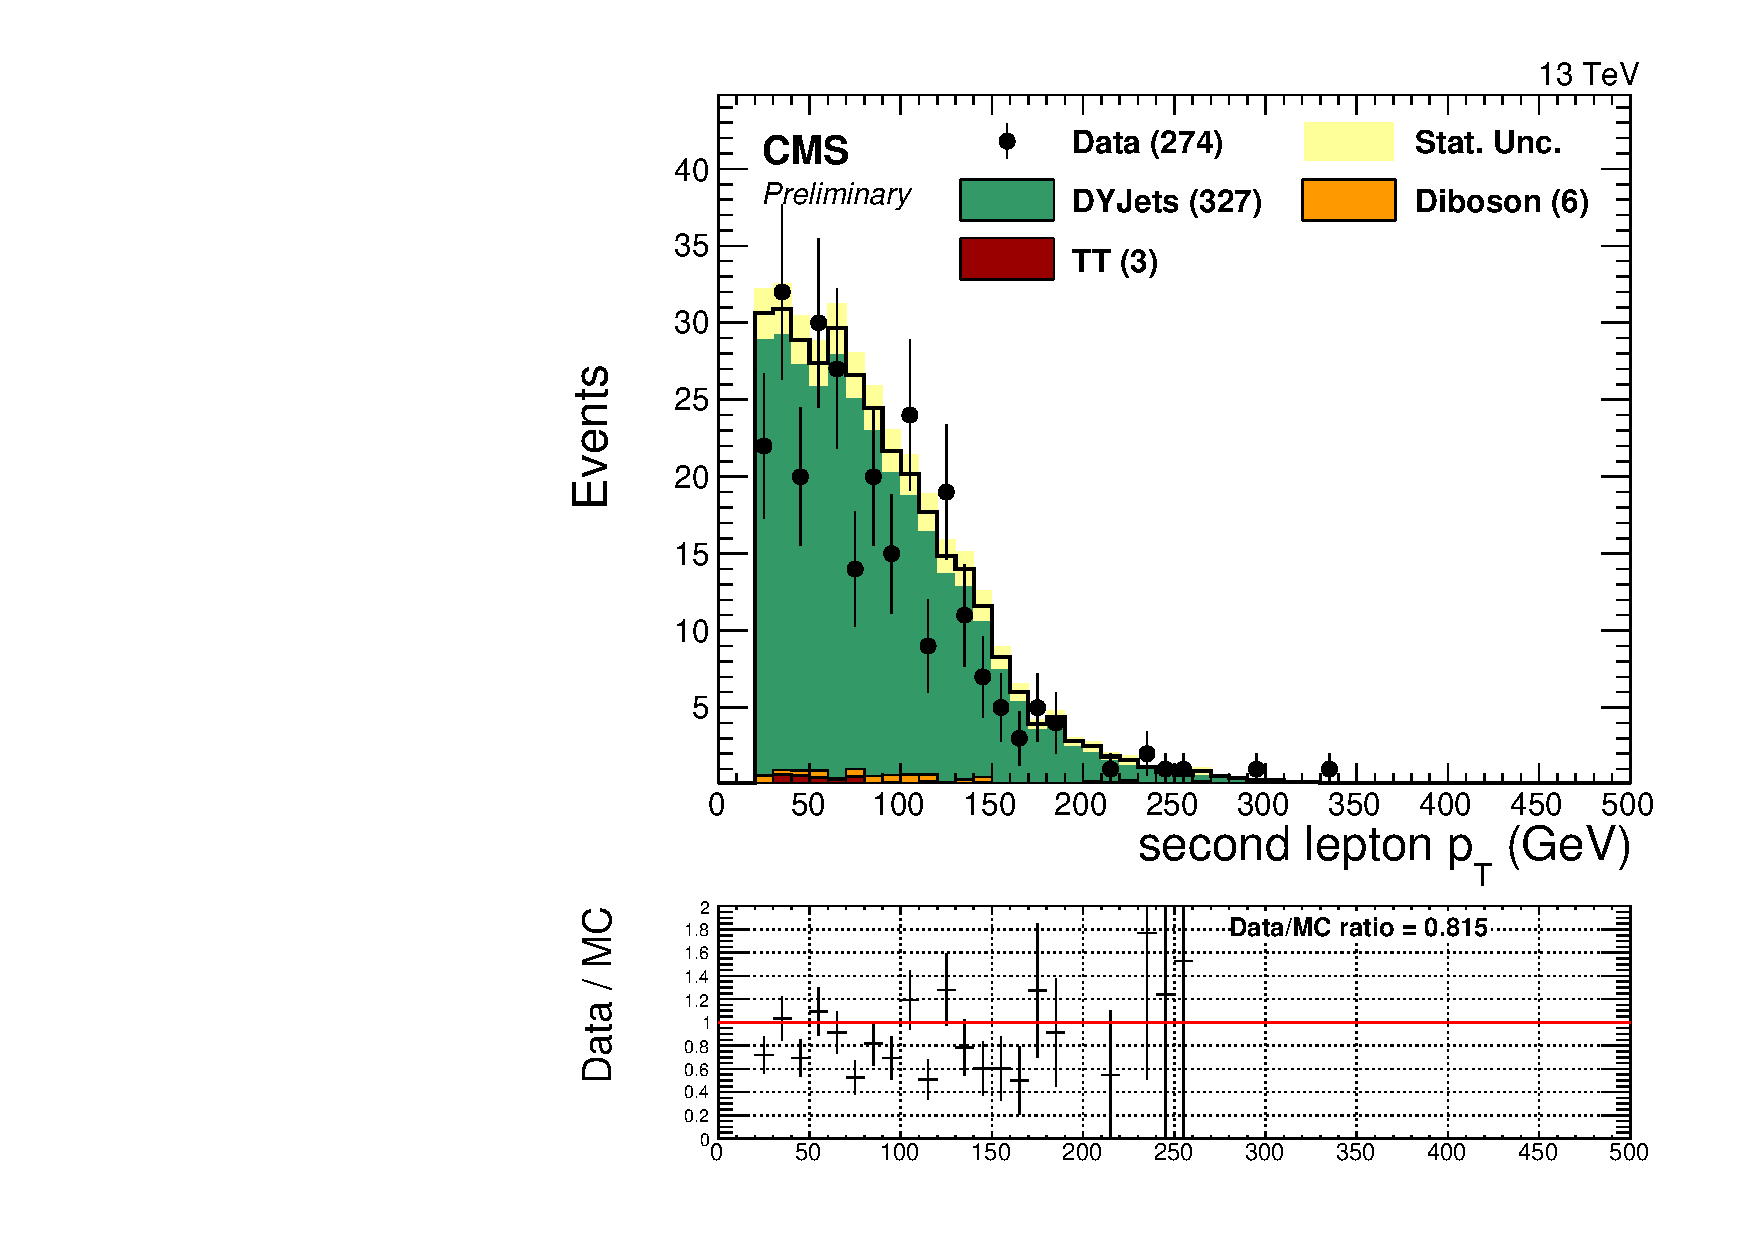
\includegraphics[scale=0.37]{figures/control/ptlep2ELP.pdf}\\[2cm]
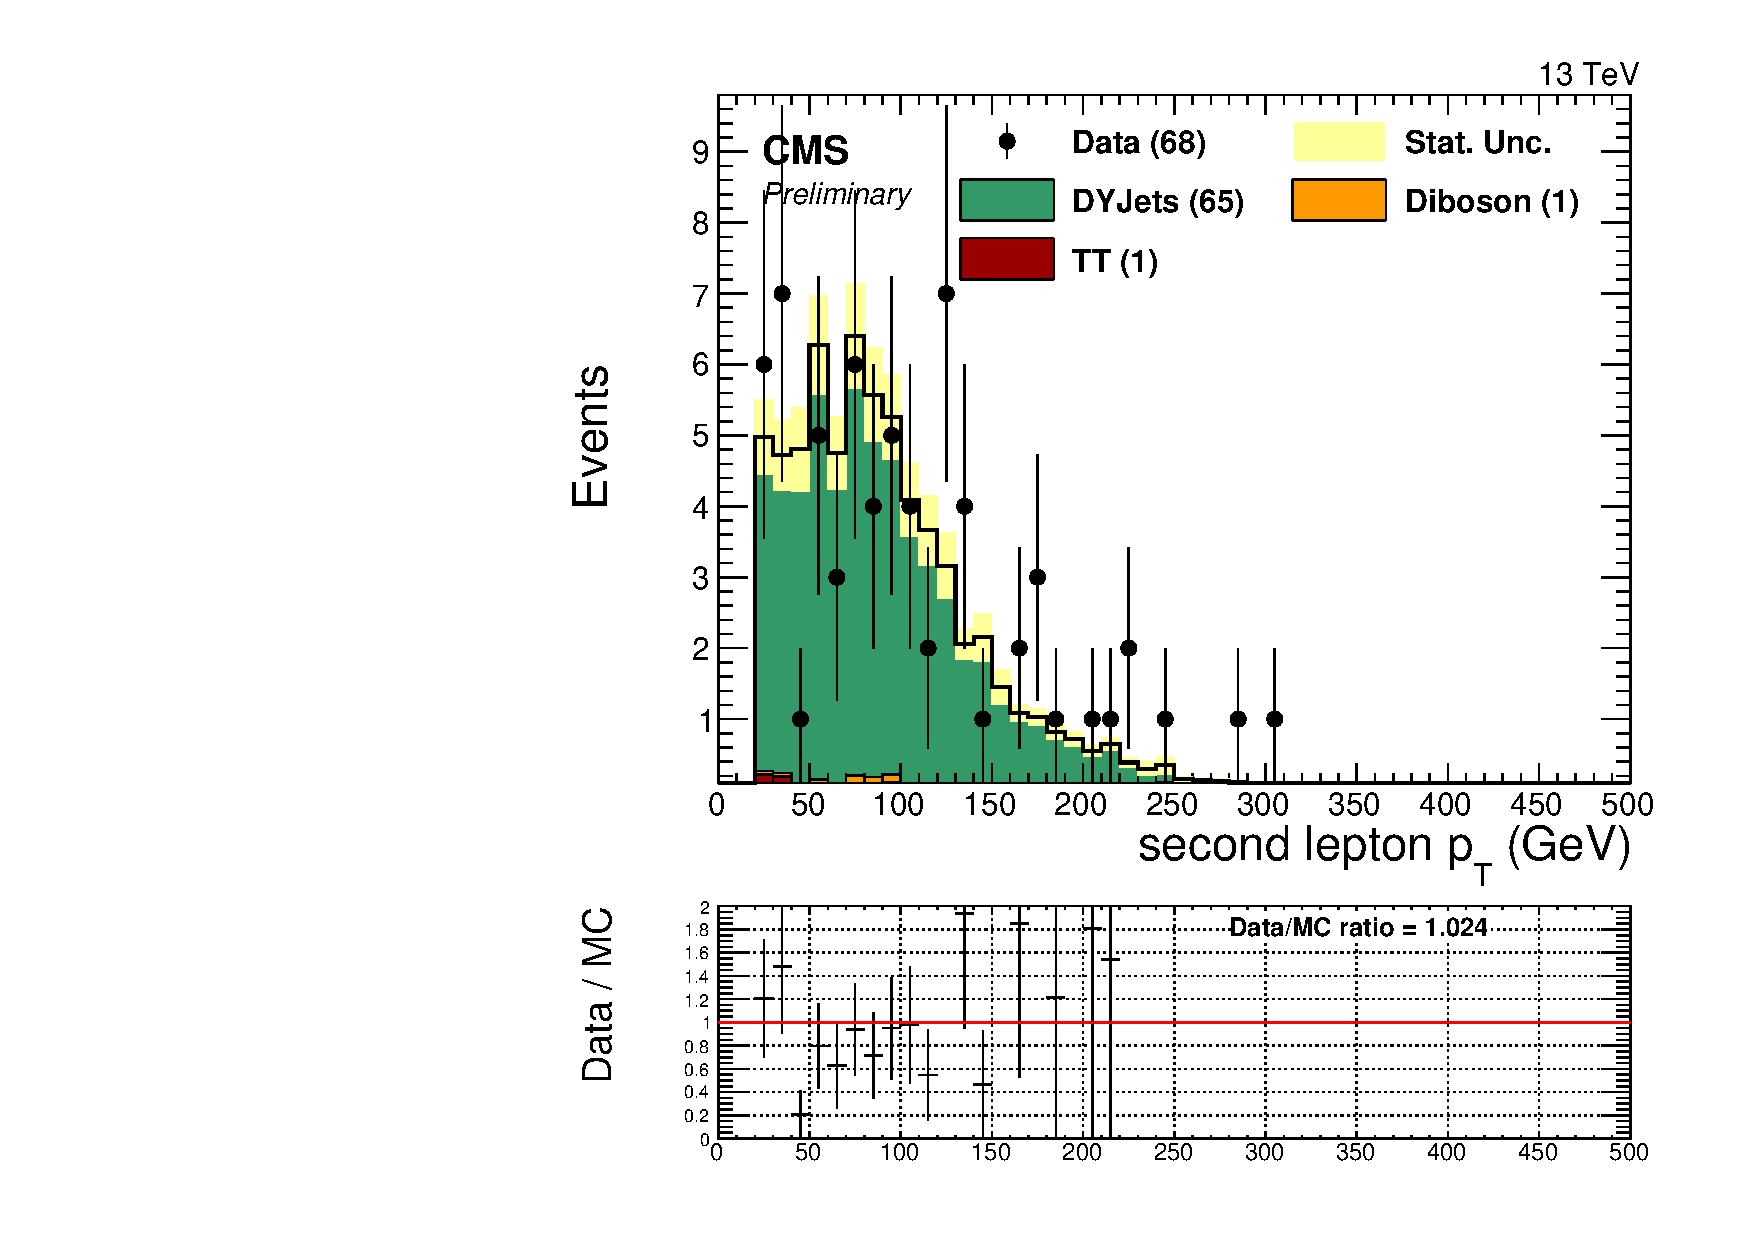
\includegraphics[scale=0.37]{figures/control/ptlep2MHP.pdf}
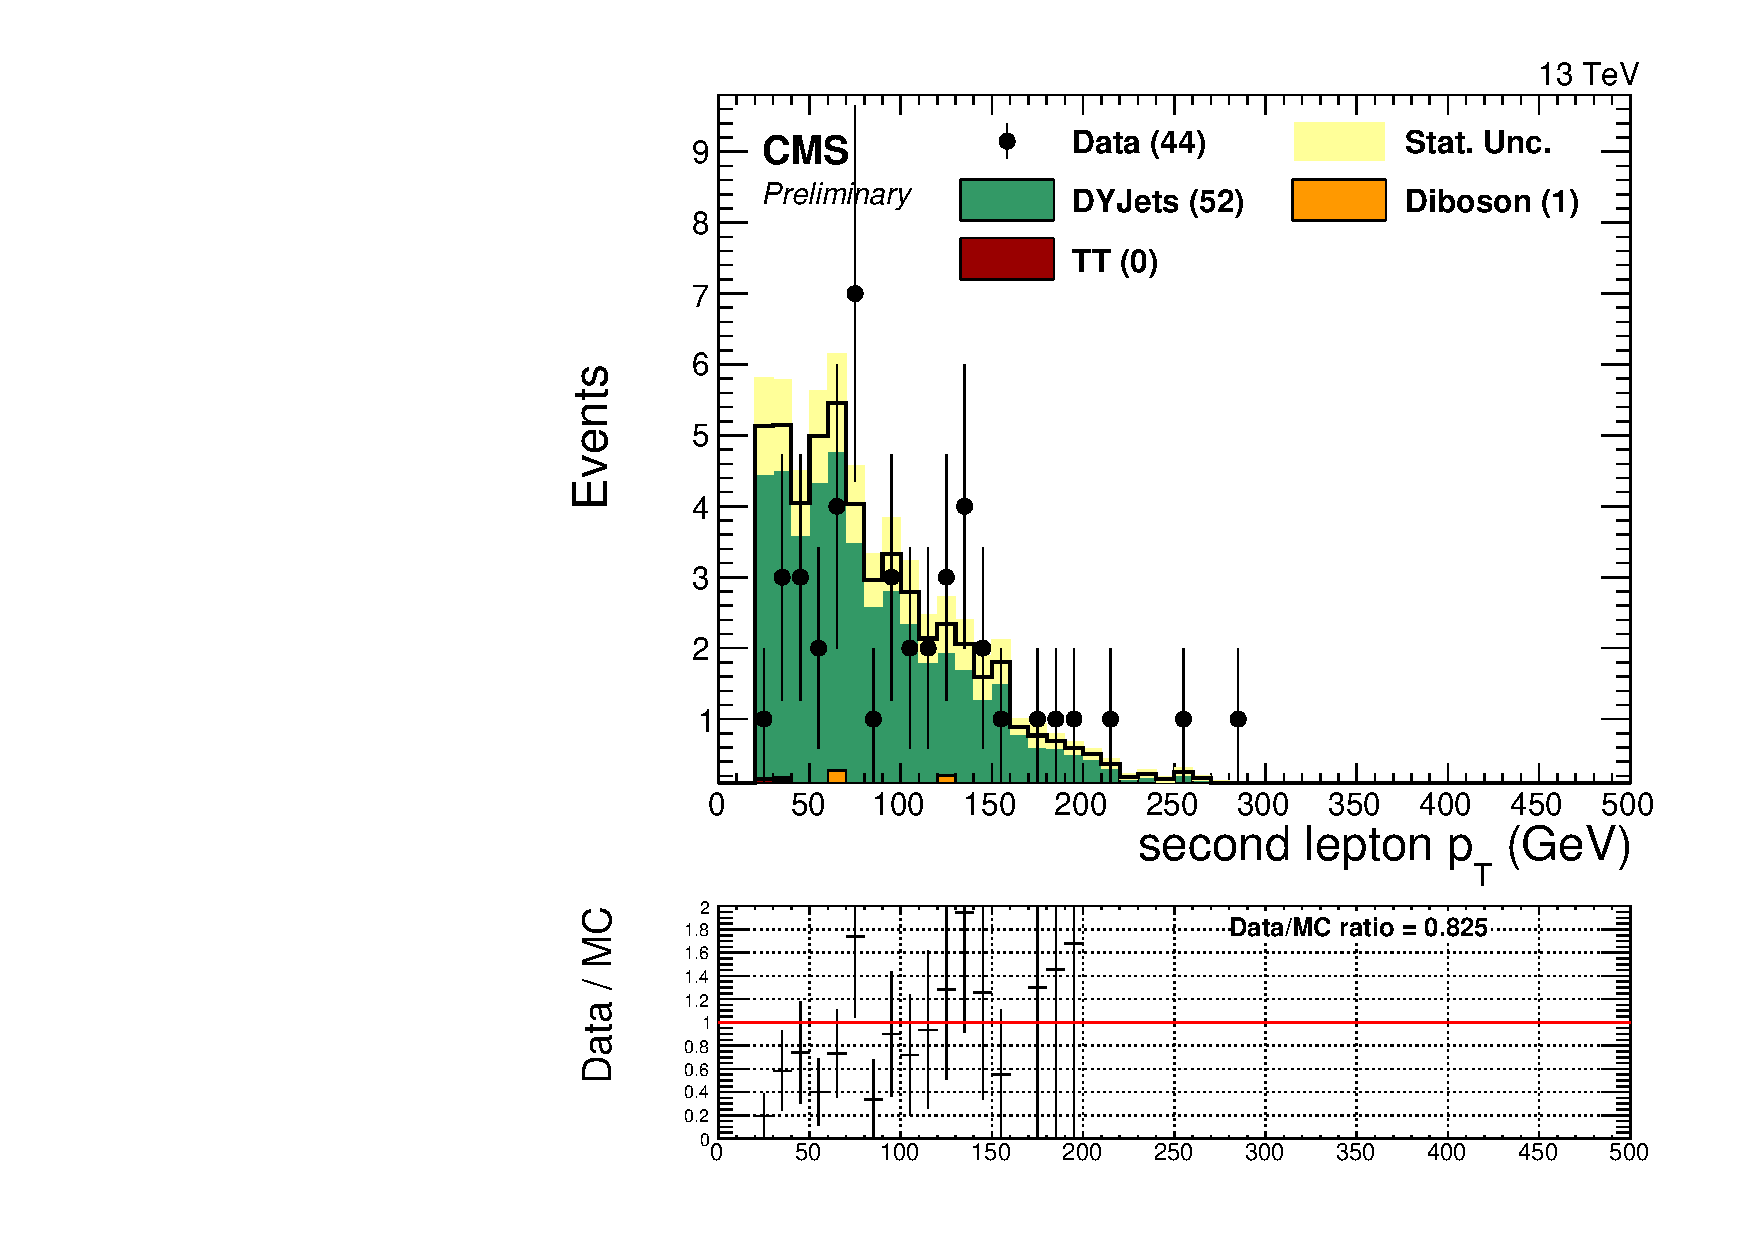
\includegraphics[scale=0.37]{figures/control/ptlep2EHP.pdf}
\caption[Distribution of \ptrans for the second lepton]{Distribution of \ptrans for the second lepton in the category: muon low purity (top-left), electron low purity (top-right), muon high purity (bottom-left), and  electron high purity (bottom-right). Simulated backgrounds are displayed as stacked histograms normalized to luminosity (2.7 fb$^{-1}$).}
\label{ptlep2_VZ}
\end{center}
\end{figure}

\begin{figure}[h]
\begin{center}
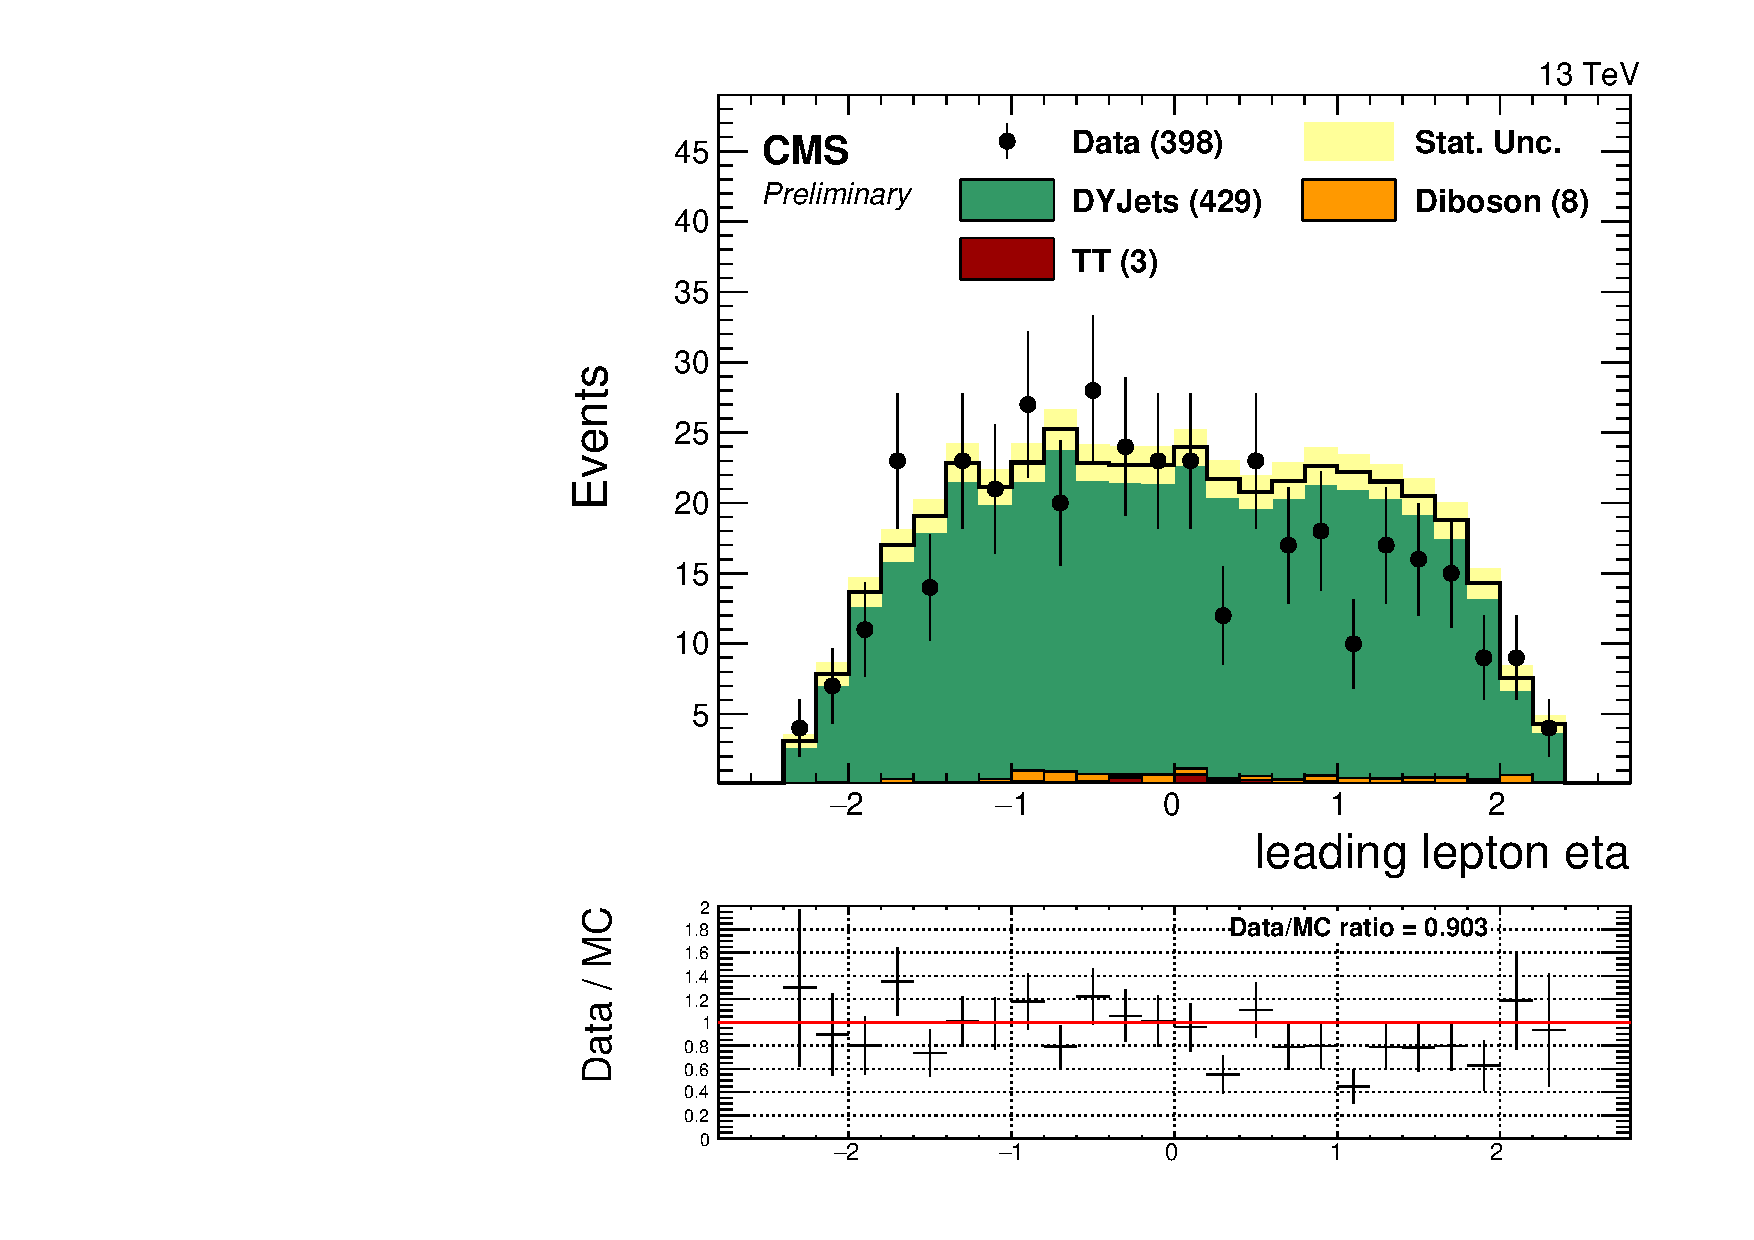
\includegraphics[scale=0.37]{figures/control/etalep1MLP.pdf}
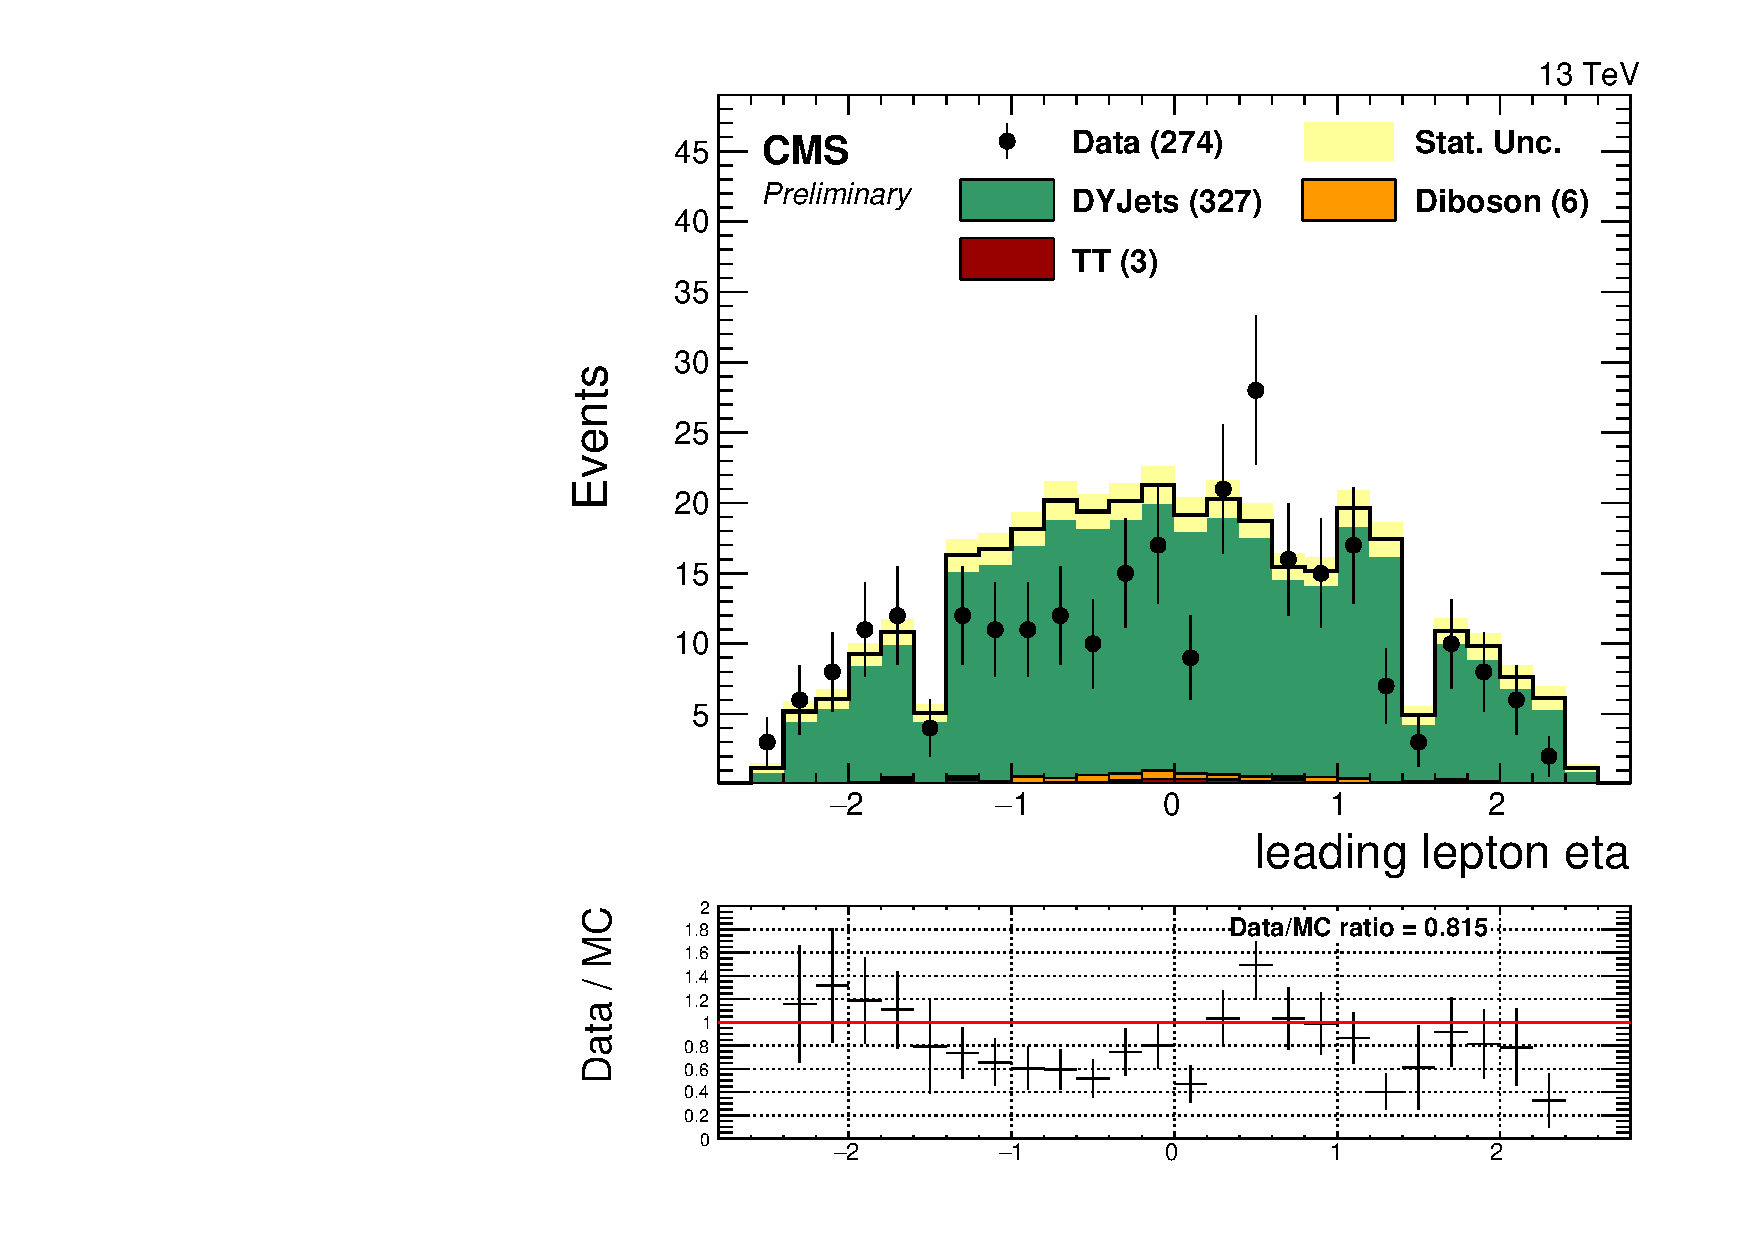
\includegraphics[scale=0.37]{figures/control/etalep1ELP.pdf}\\[2cm]
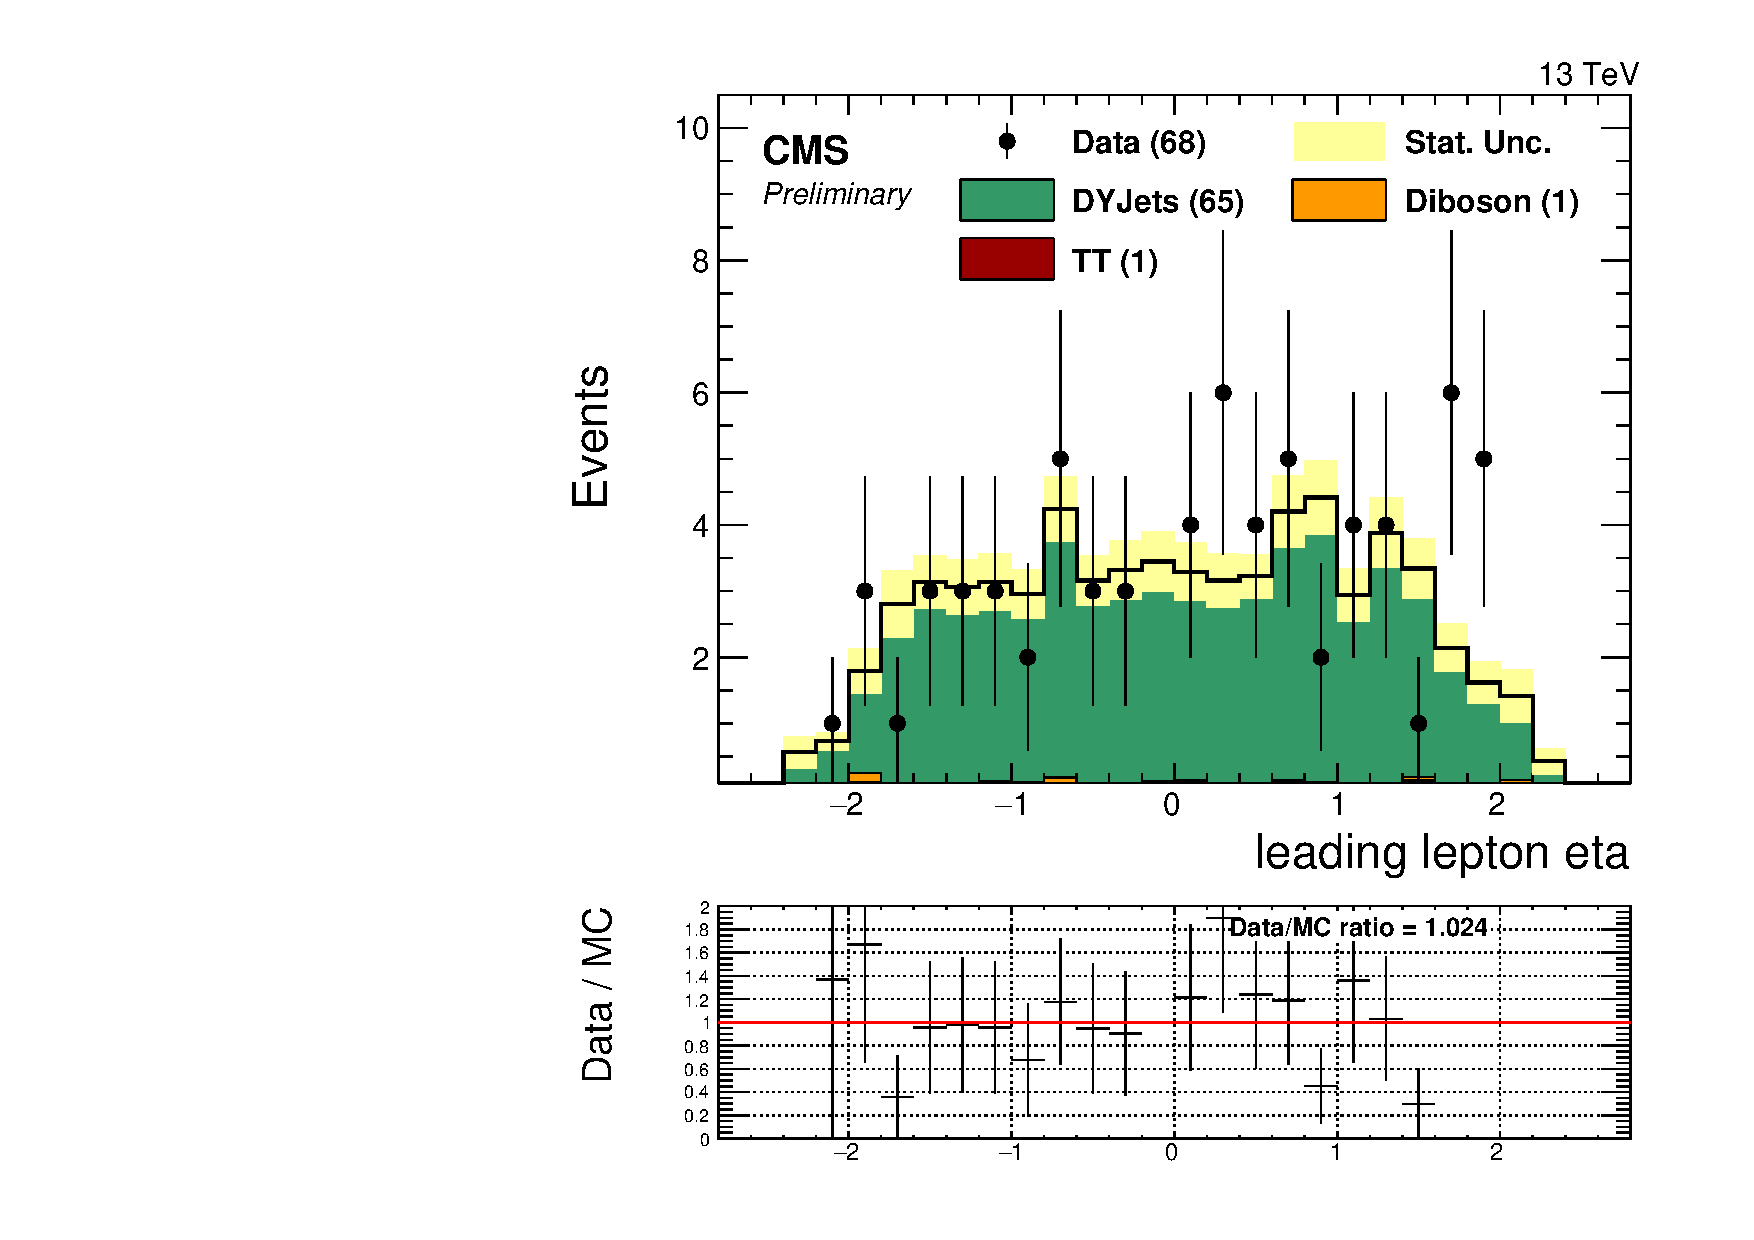
\includegraphics[scale=0.37]{figures/control/etalep1MHP.pdf}
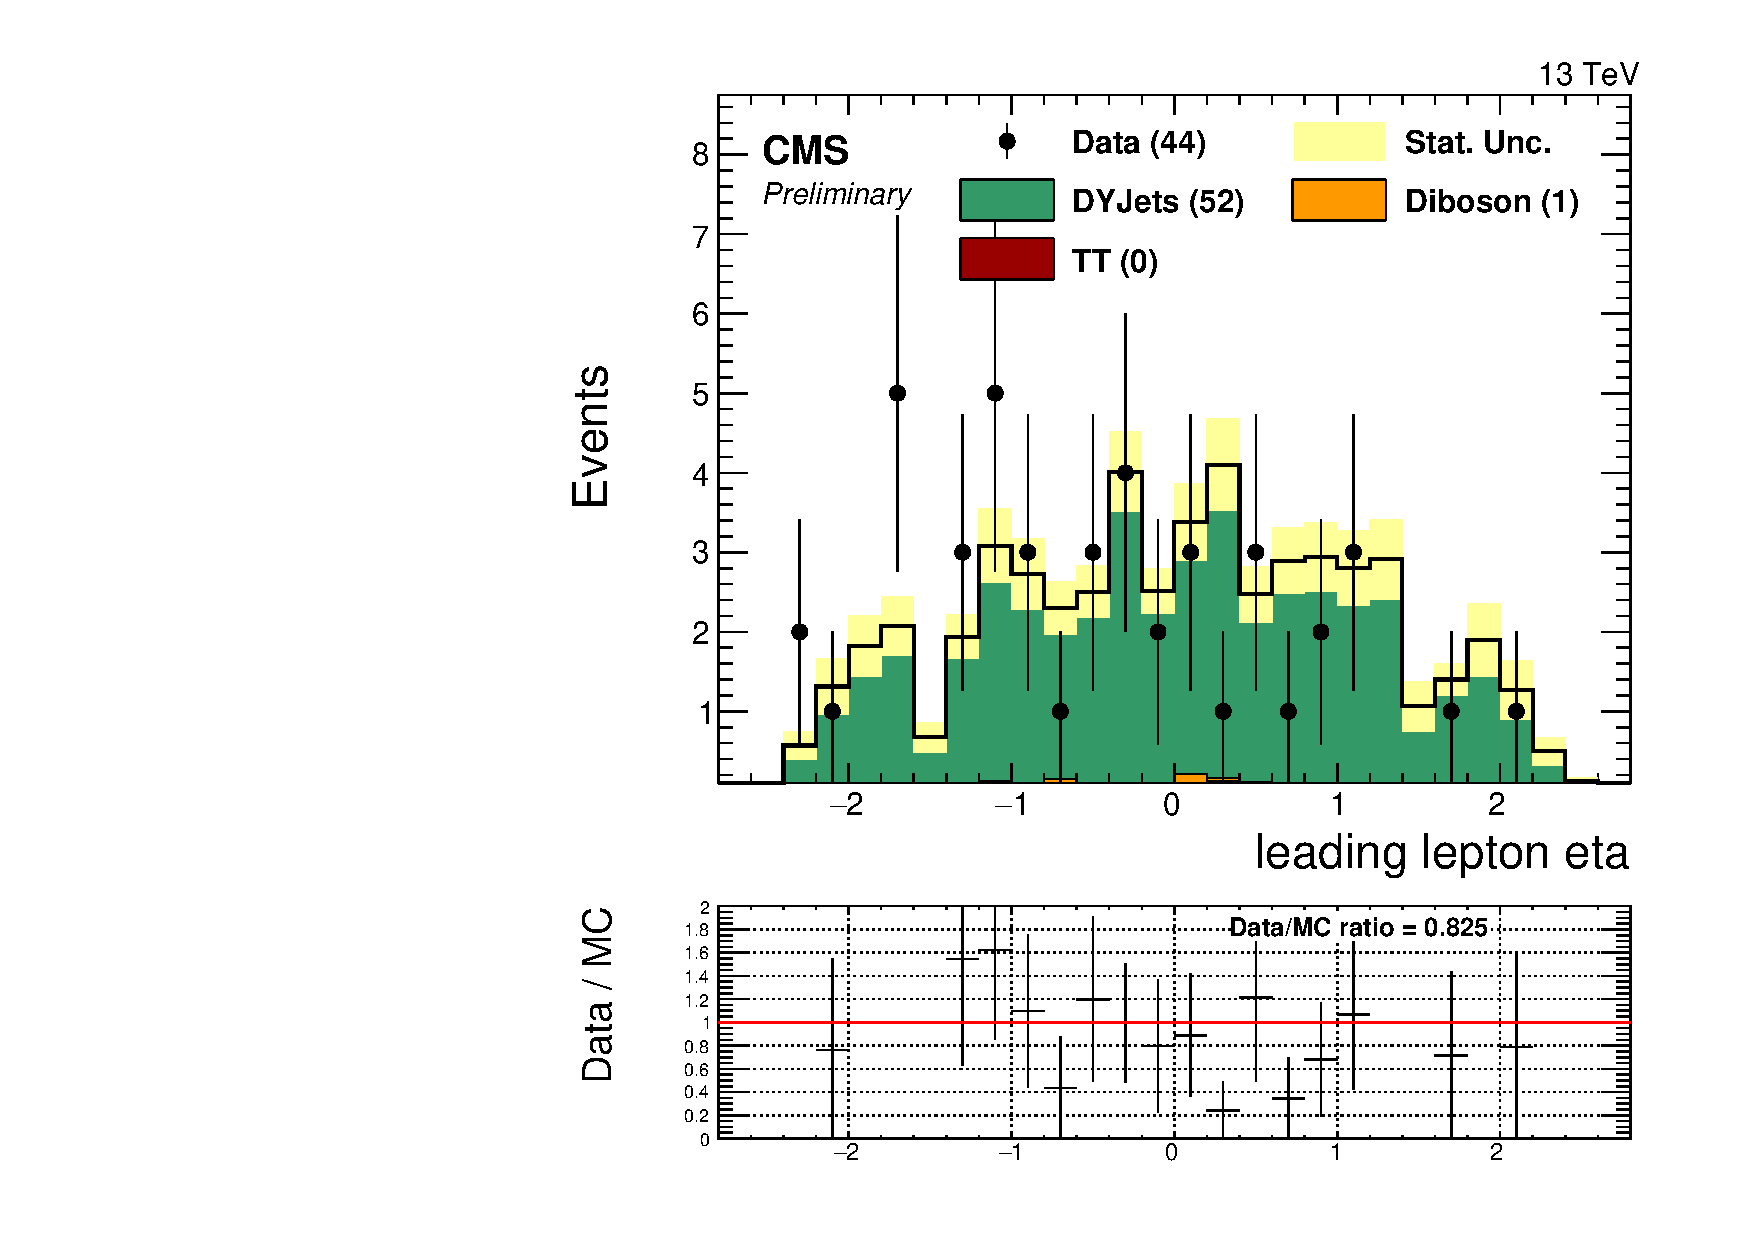
\includegraphics[scale=0.37]{figures/control/etalep1EHP.pdf}
\caption[Distribution of $\eta$ for the leading lepton]{Distribution of $\eta$ for the leading lepton in the category: muon low purity (top-left), electron low purity (top-right), muon high purity (bottom-left), and  electron high purity (bottom-right). Simulated backgrounds are displayed as stacked histograms normalized to luminosity (2.7 fb$^{-1}$).}
\label{etalep1_VZ}
\end{center}
\end{figure}
\begin{figure}[h]
\begin{center}
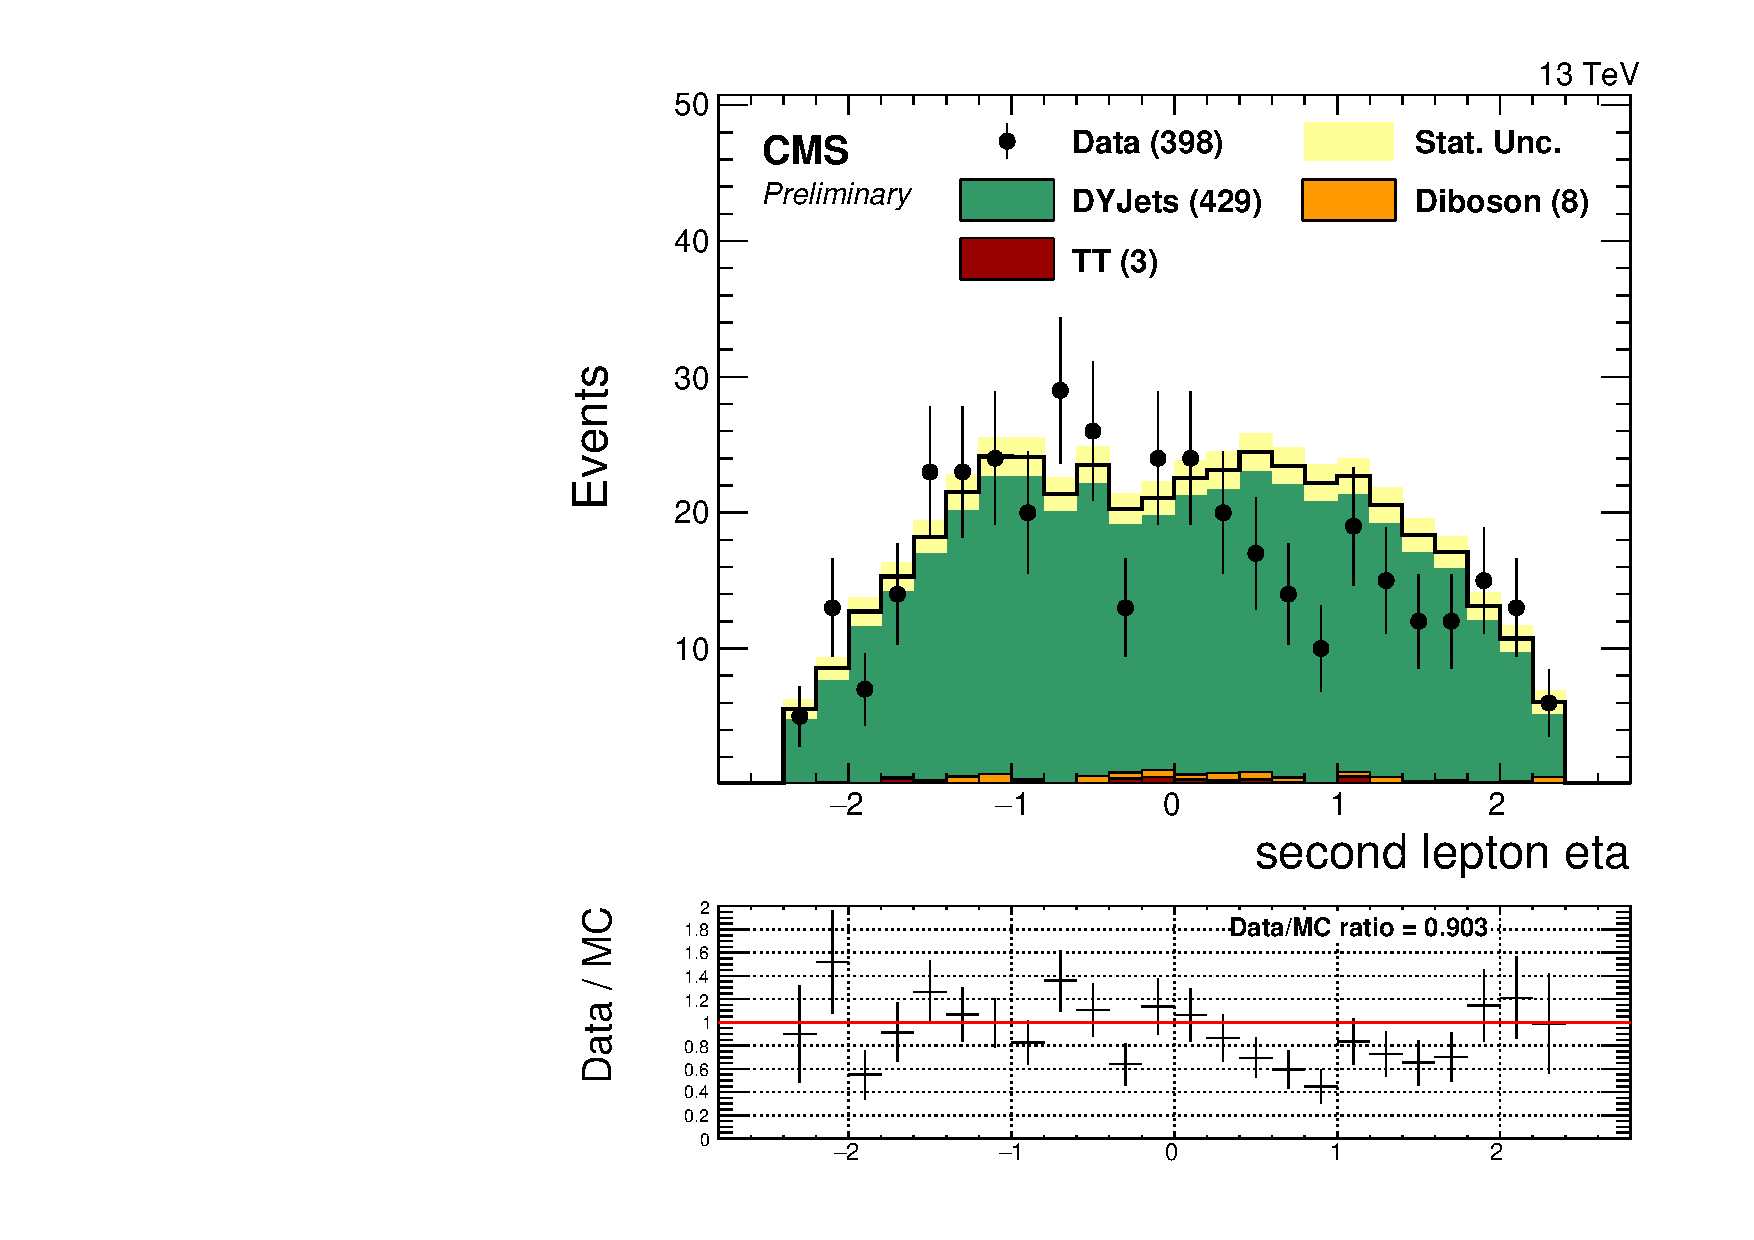
\includegraphics[scale=0.37]{figures/control/etalep2MLP.pdf}
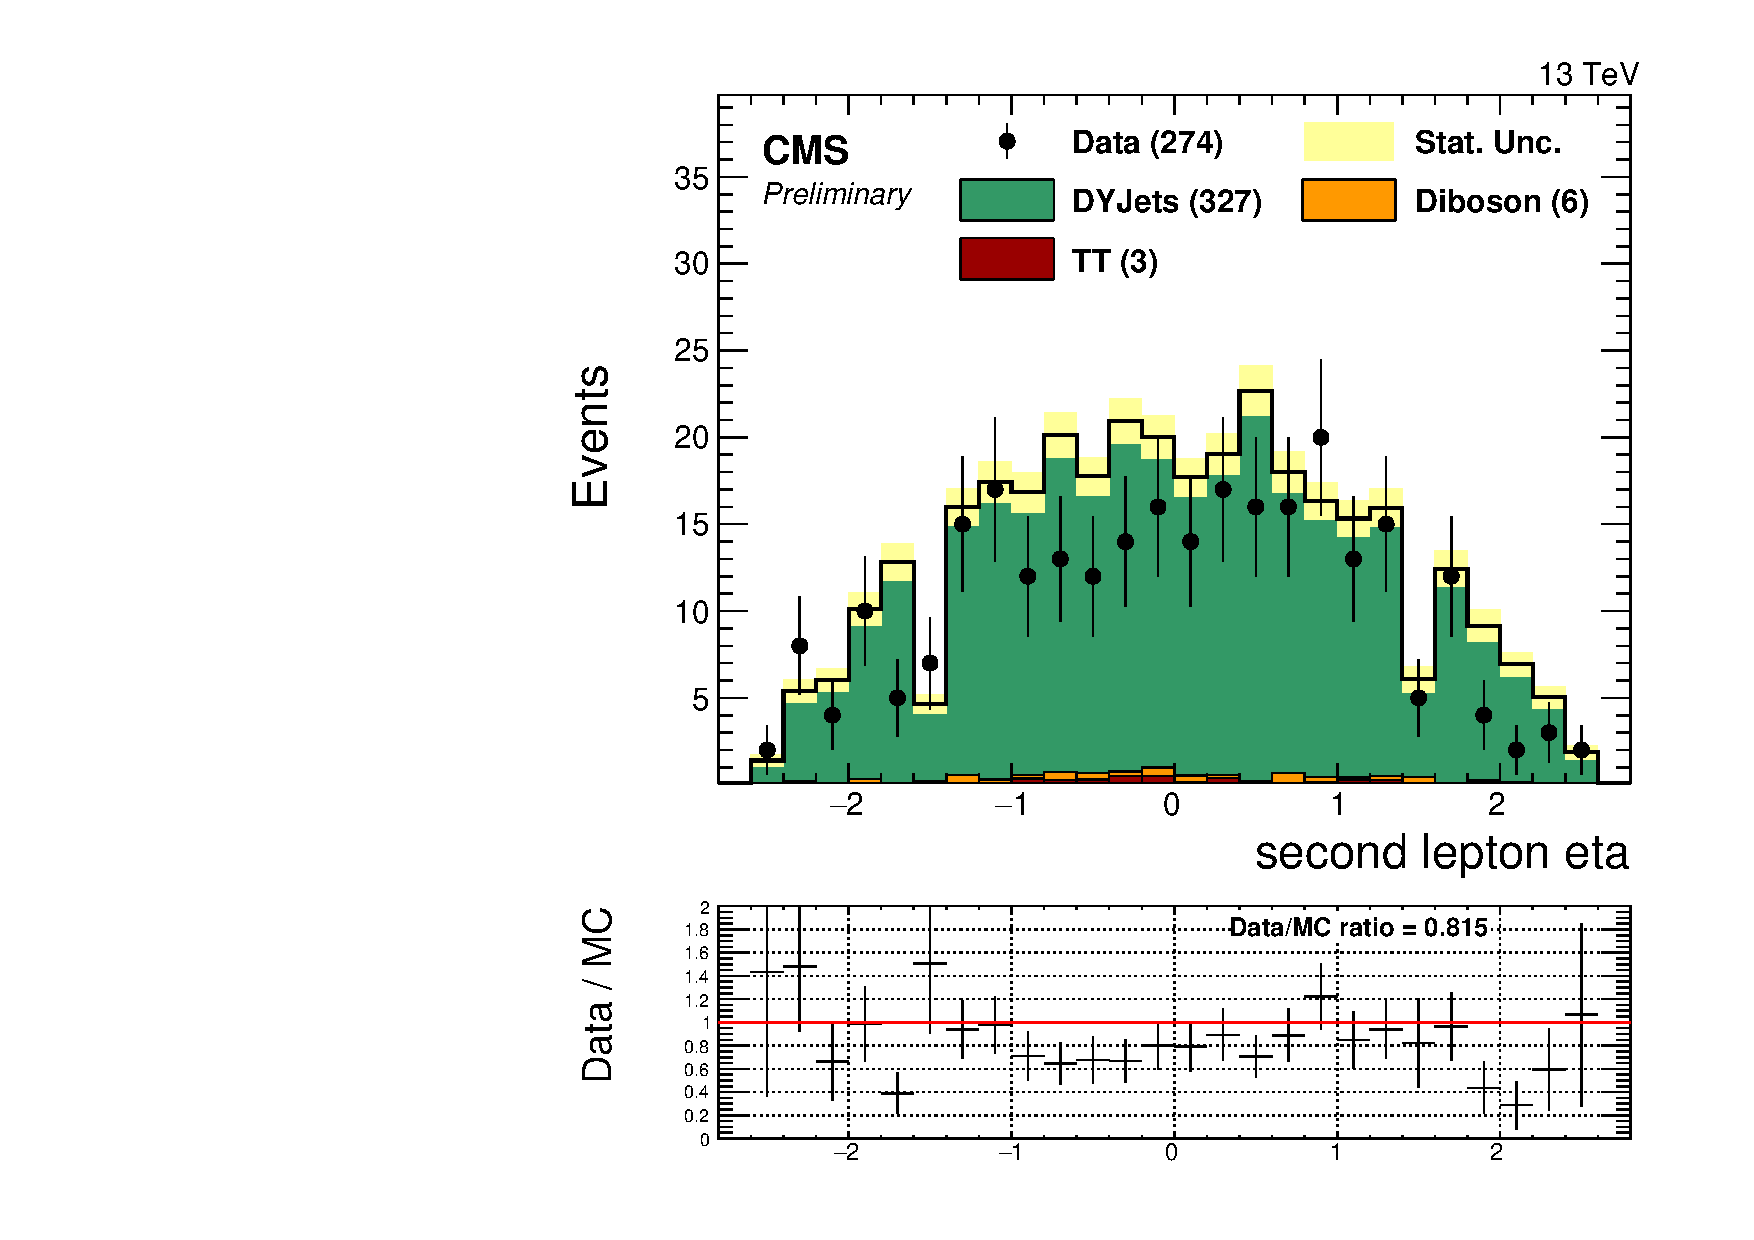
\includegraphics[scale=0.37]{figures/control/etalep2ELP.pdf}\\[2cm]
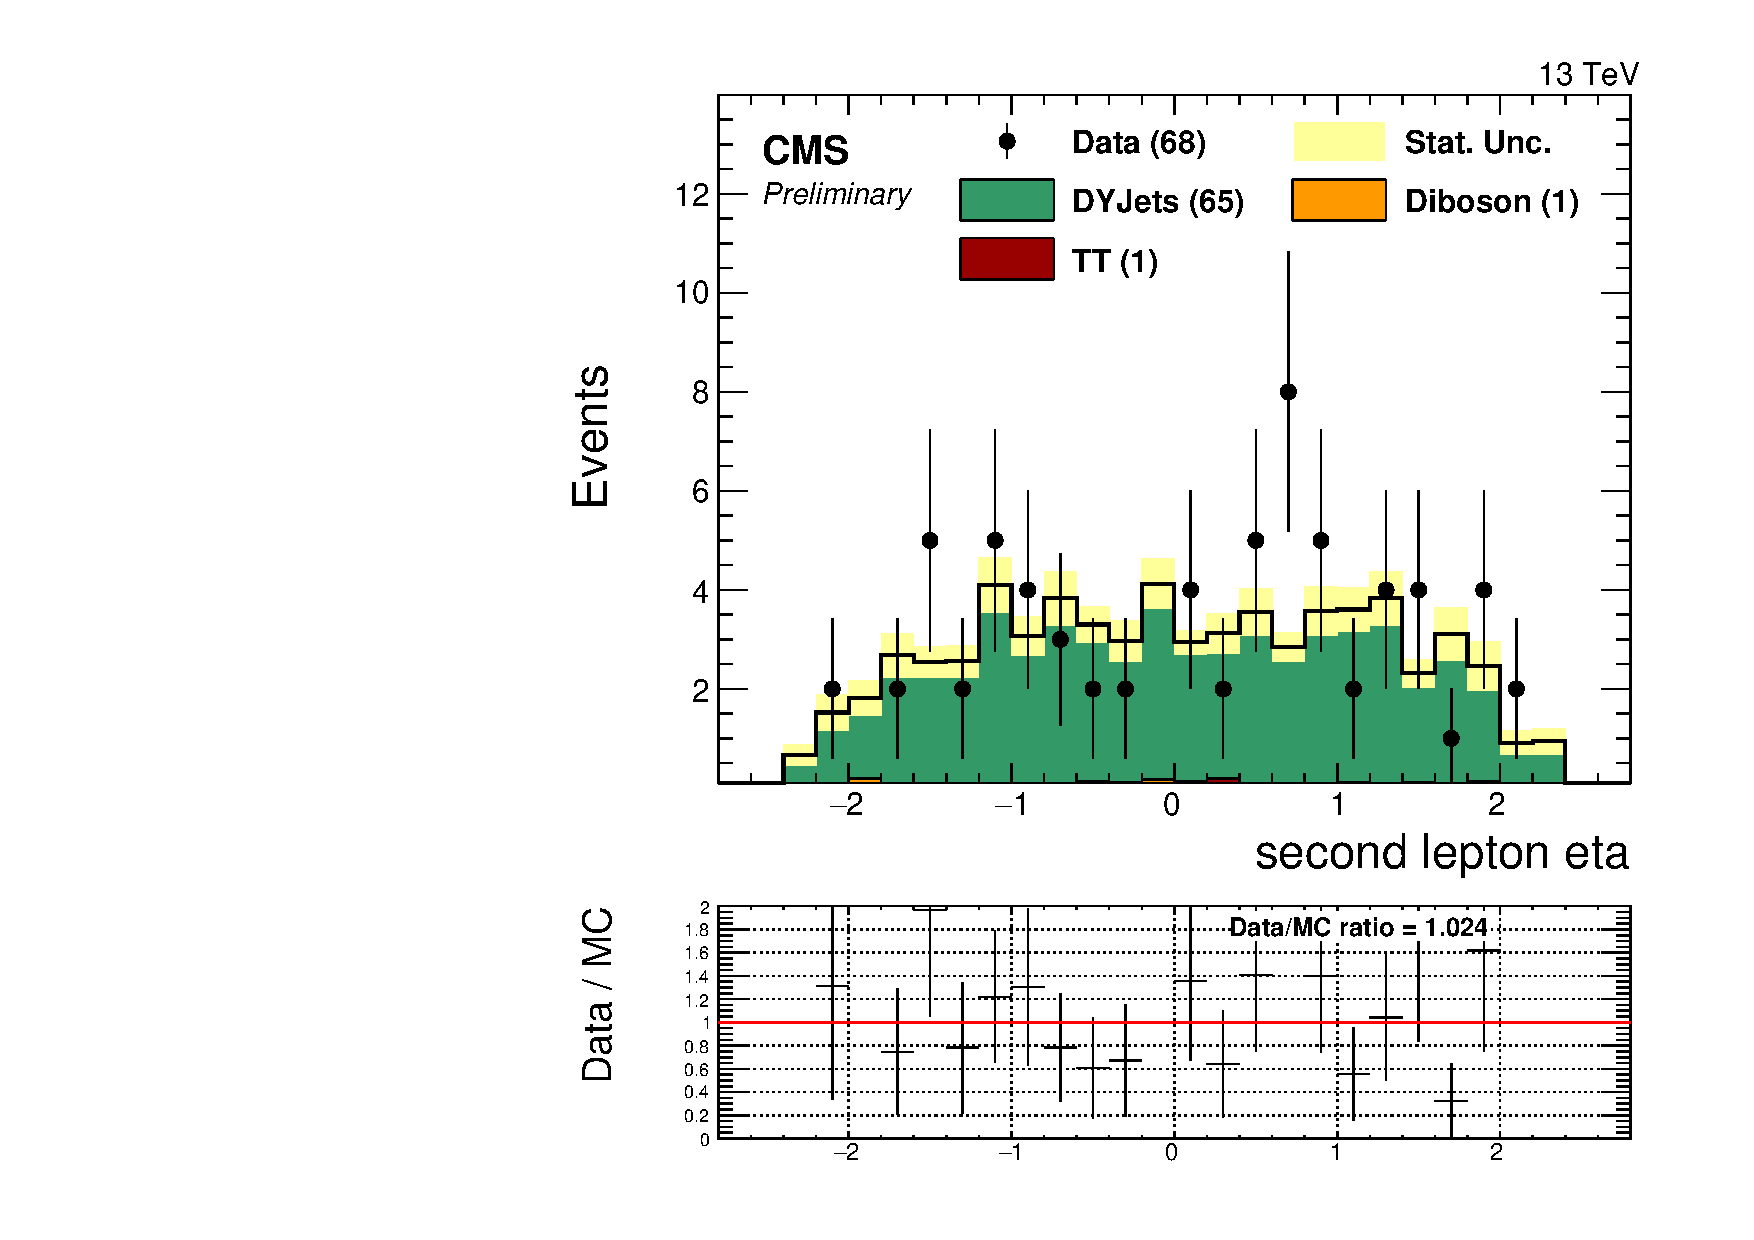
\includegraphics[scale=0.37]{figures/control/etalep2MHP.pdf}
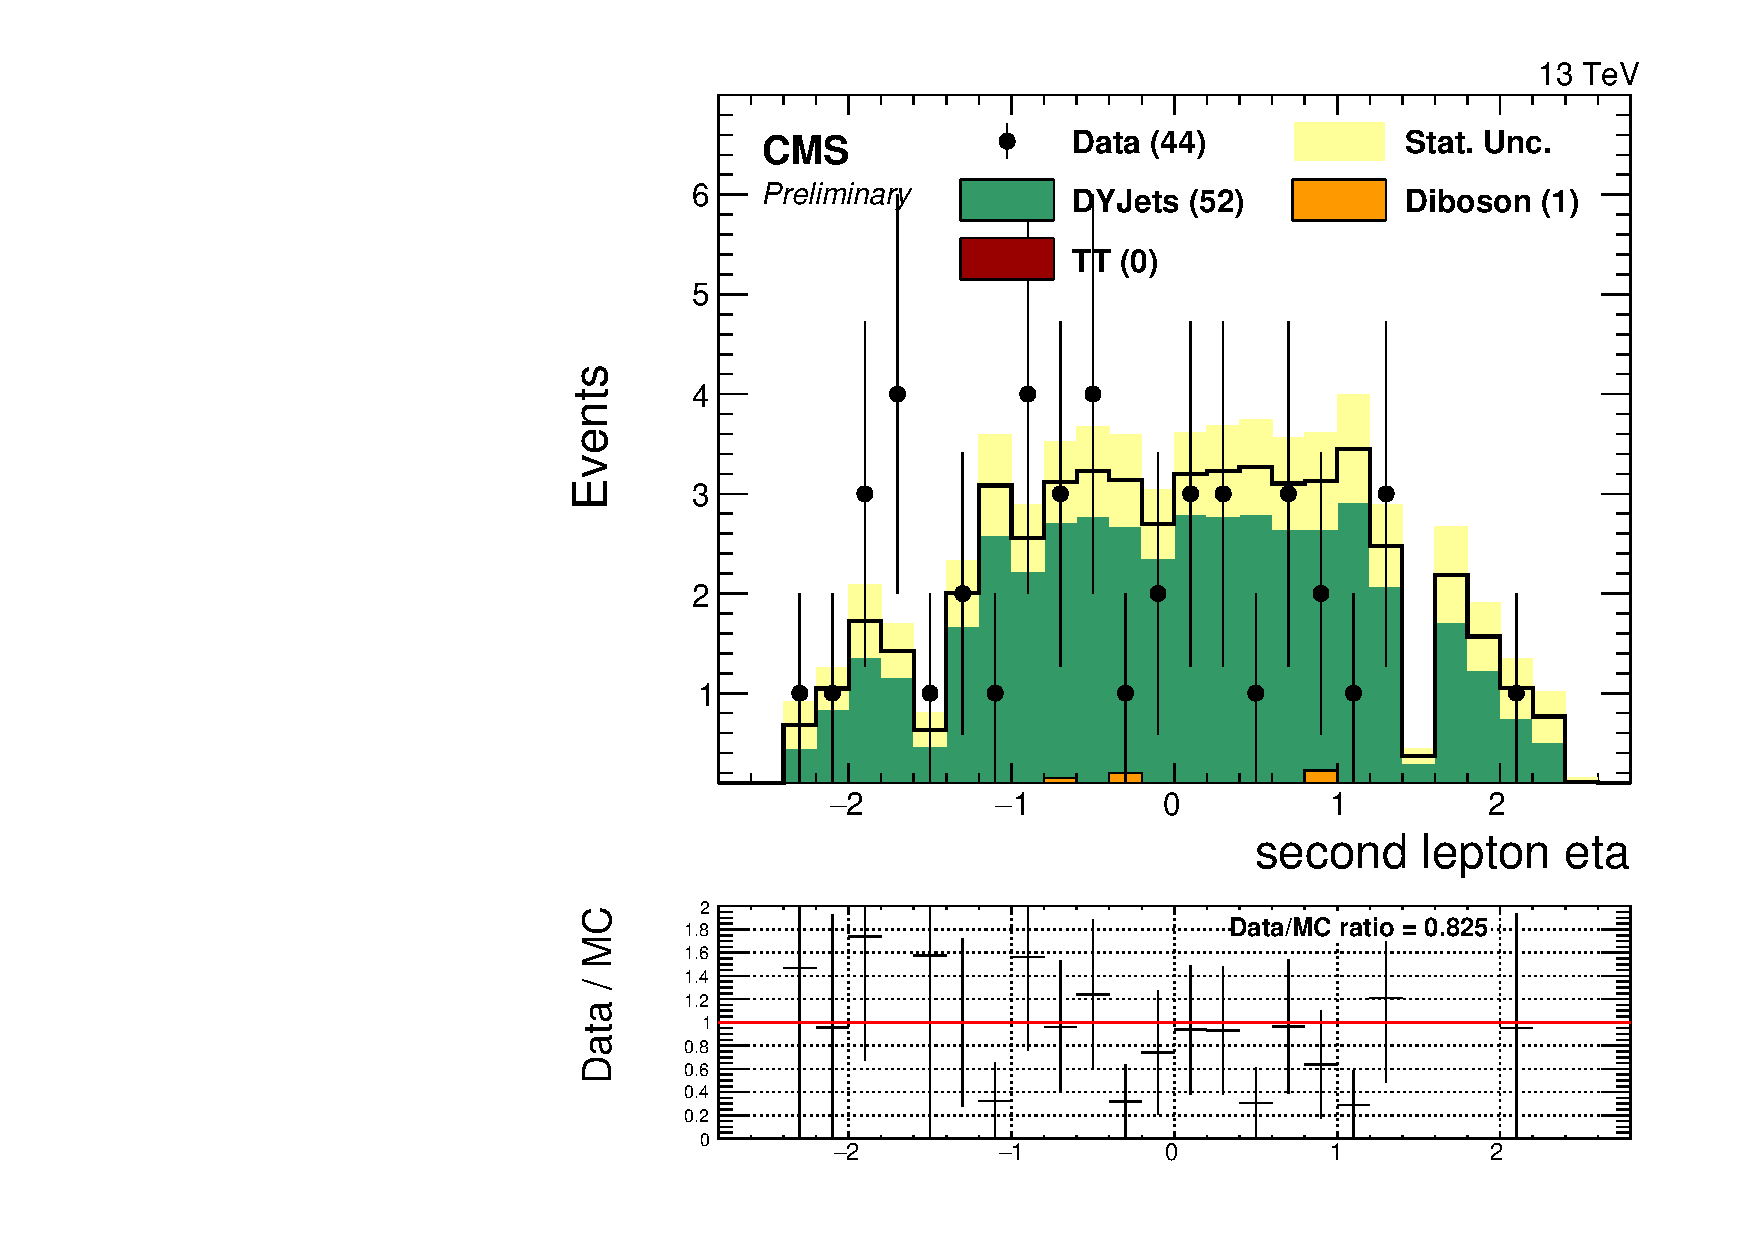
\includegraphics[scale=0.37]{figures/control/etalep2EHP.pdf}
\caption[Distribution of $\eta$ for the second lepton]{Distribution of $\eta$ for the second lepton in the category: muon low purity (top-left), electron low purity (top-right), muon high purity (bottom-left), and  electron high purity (bottom-right). Simulated backgrounds are displayed as stacked histograms normalized to luminosity (2.7 fb$^{-1}$).}
\label{etalep2_VZ}
\end{center}
\end{figure}

\begin{figure}[h]
\begin{center}
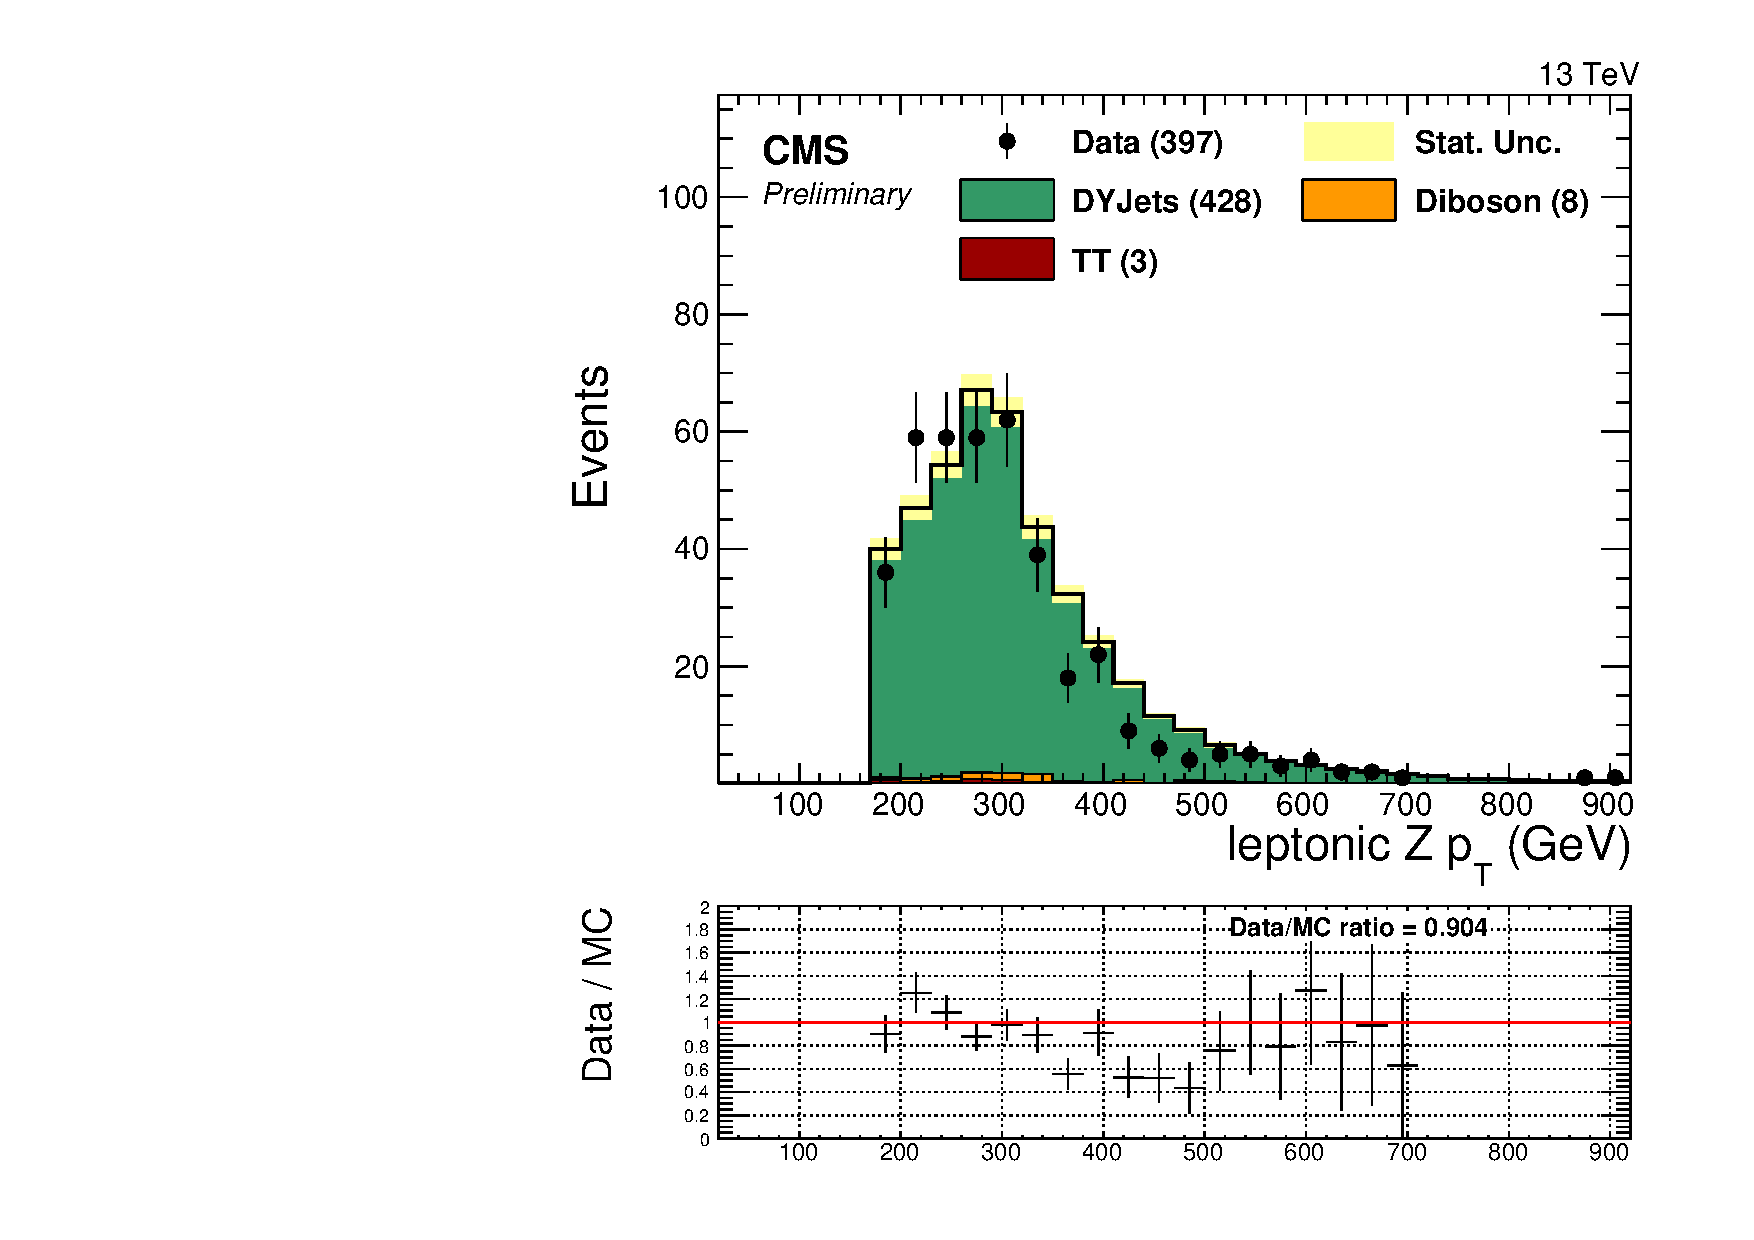
\includegraphics[scale=0.37]{figures/control/ptZllMLP.pdf}
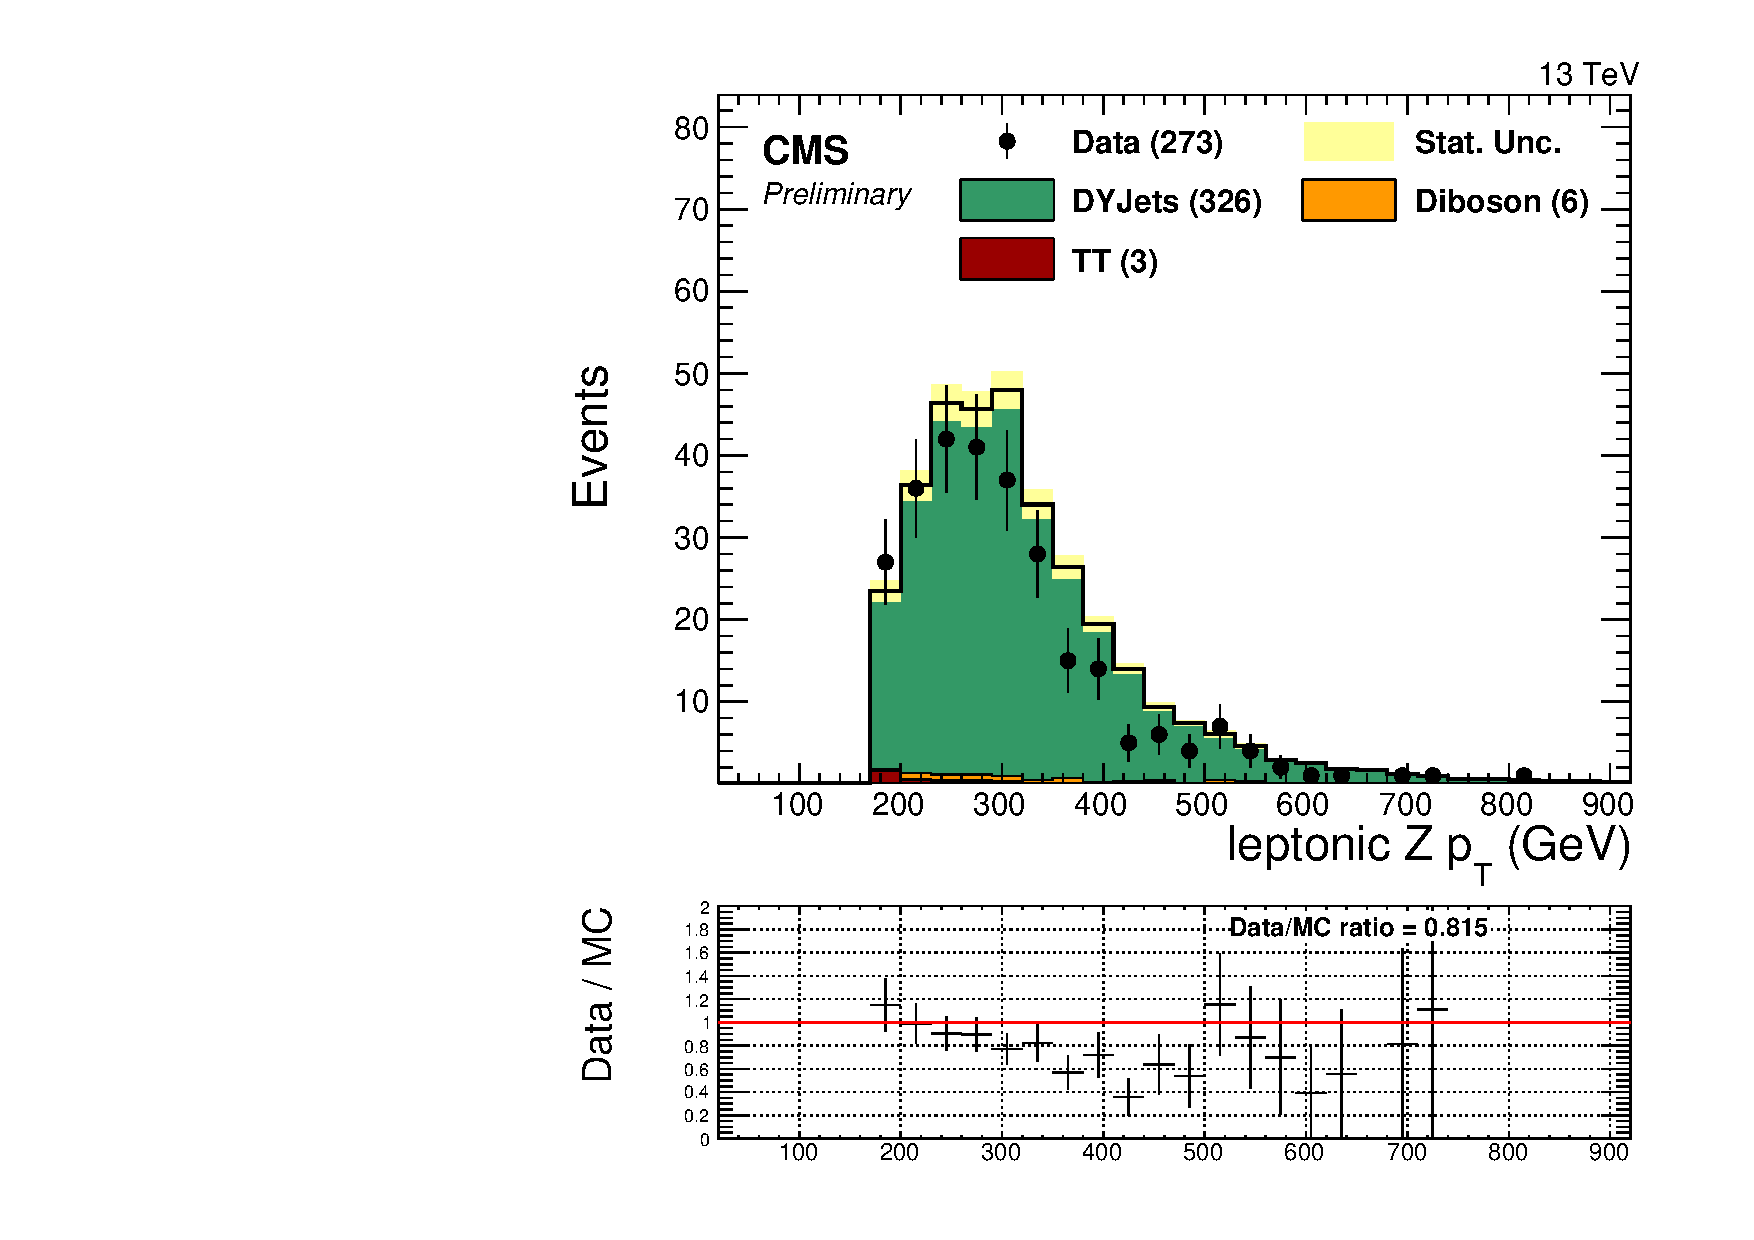
\includegraphics[scale=0.37]{figures/control/ptZllELP.pdf}\\[2cm]
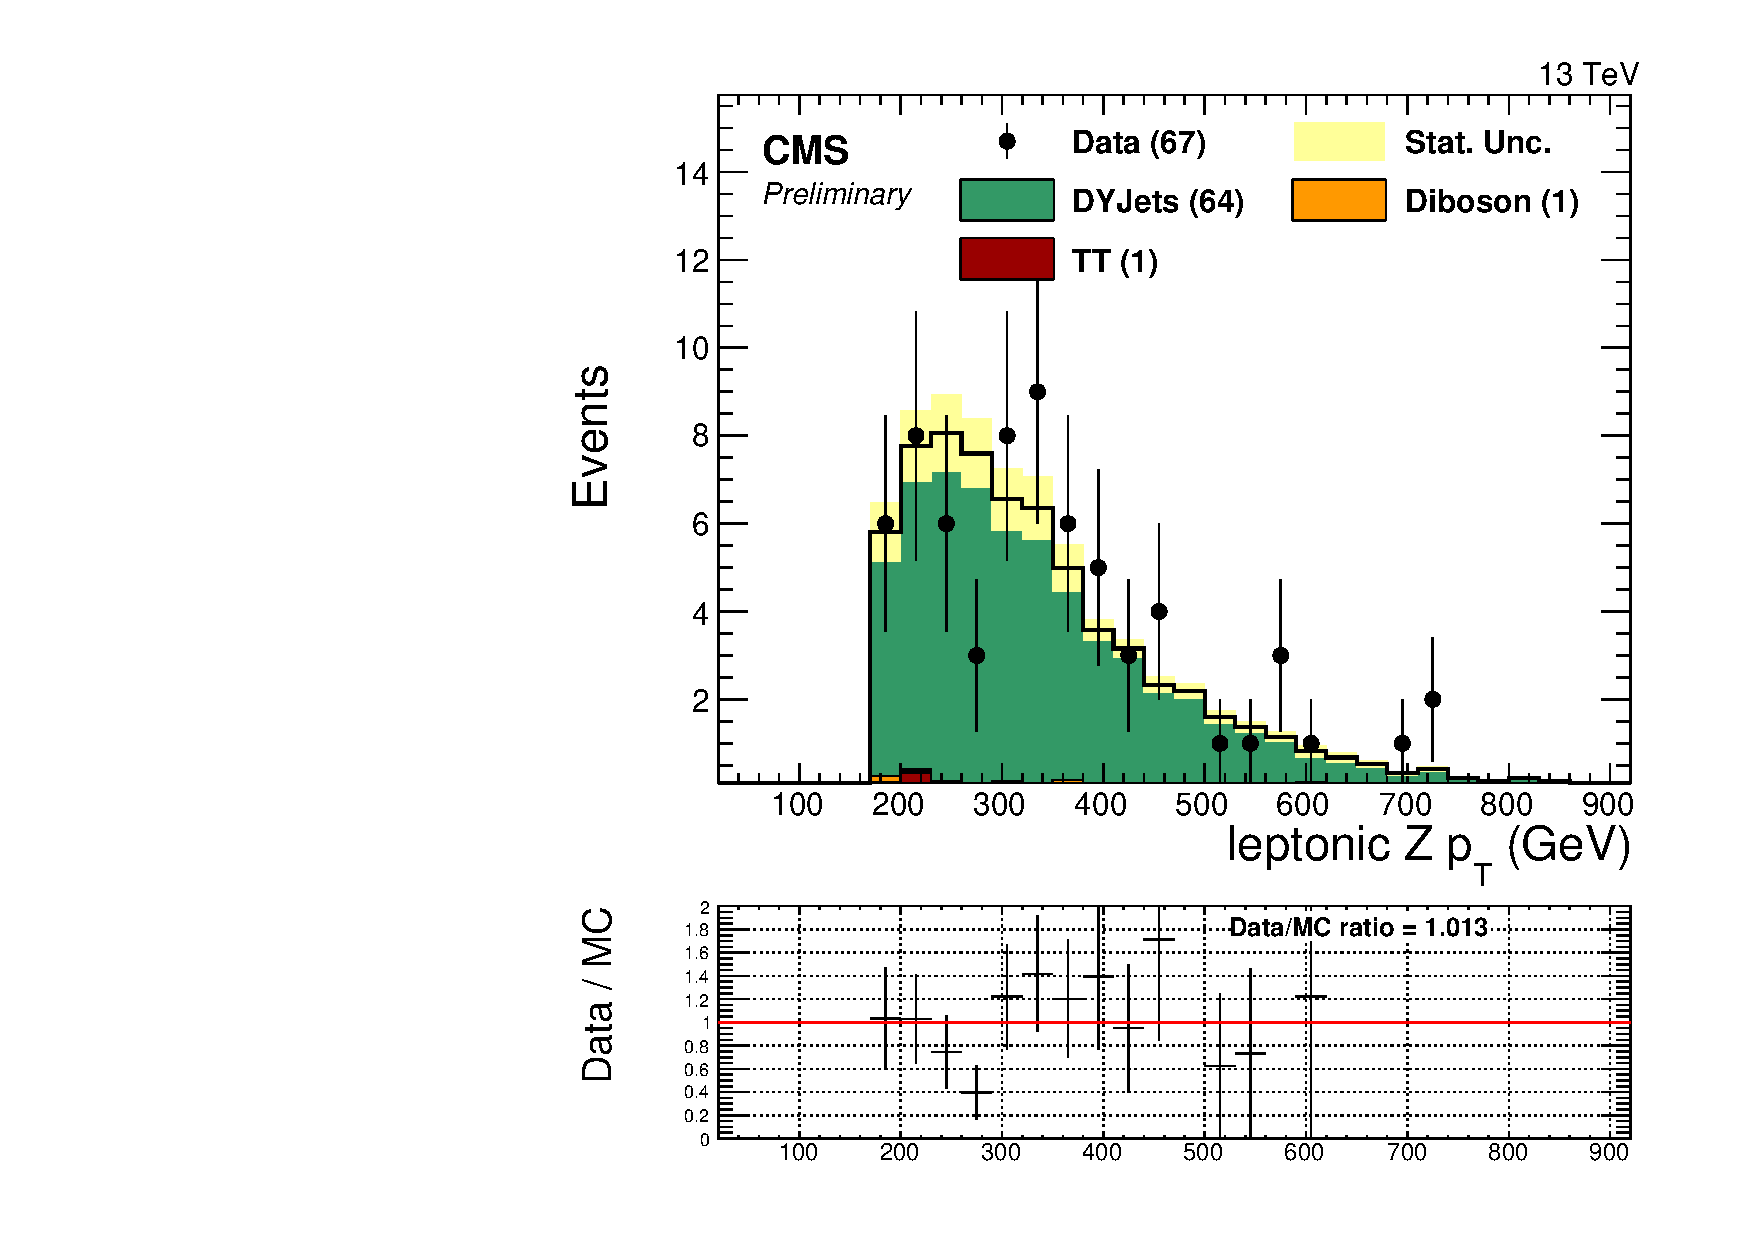
\includegraphics[scale=0.37]{figures/control/ptZllMHP.pdf}
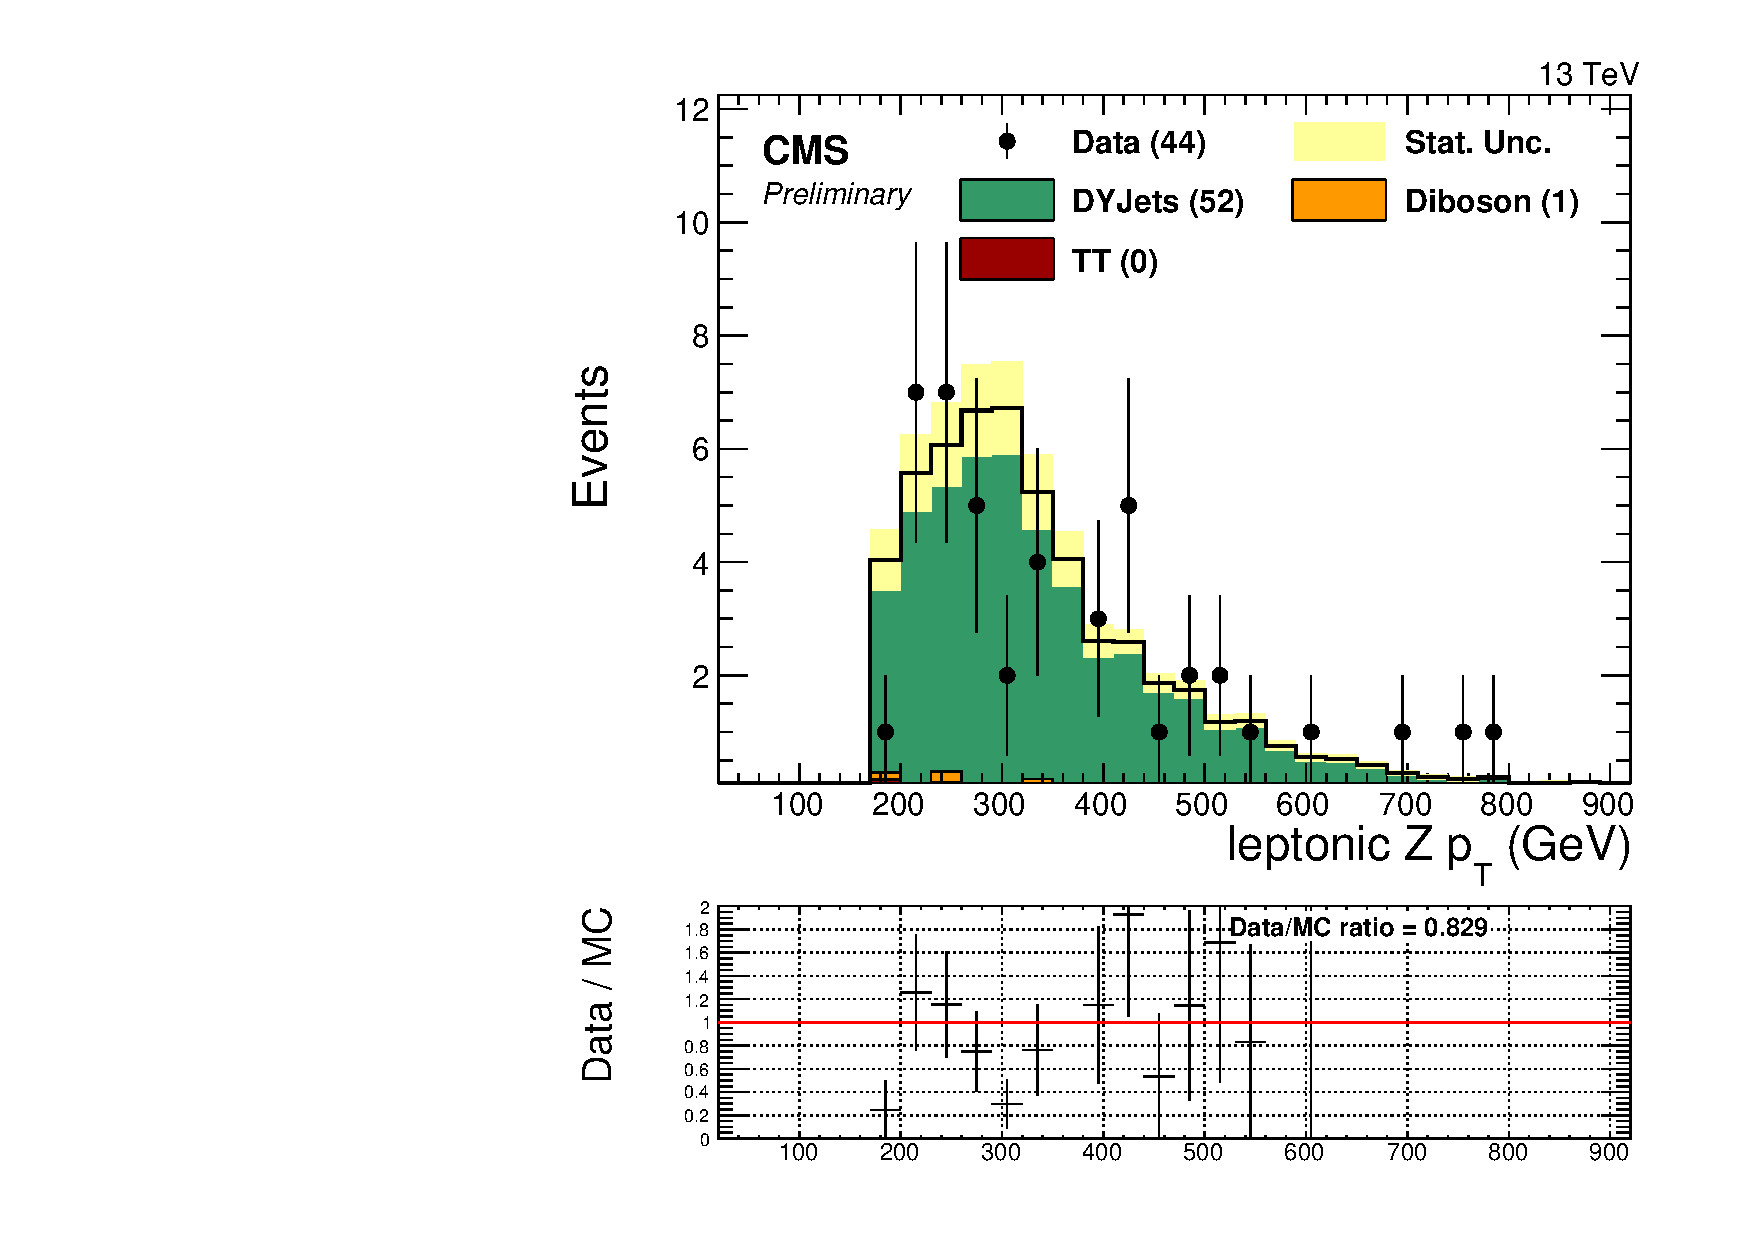
\includegraphics[scale=0.37]{figures/control/ptZllEHP.pdf}
\caption[Distribution of \ptrans of the leptonic Z candidate]{Distribution of \ptrans of the leptonic Z candidate in the category: muon low purity (top-left), electron low purity (top-right), muon high purity (bottom-left), and  electron high purity (bottom-right). Simulated backgrounds are displayed as stacked histograms normalized to luminosity (2.7 fb$^{-1}$).}
\label{ptZll_VZ}
\end{center}
\end{figure}
\begin{figure}[h]
\begin{center}
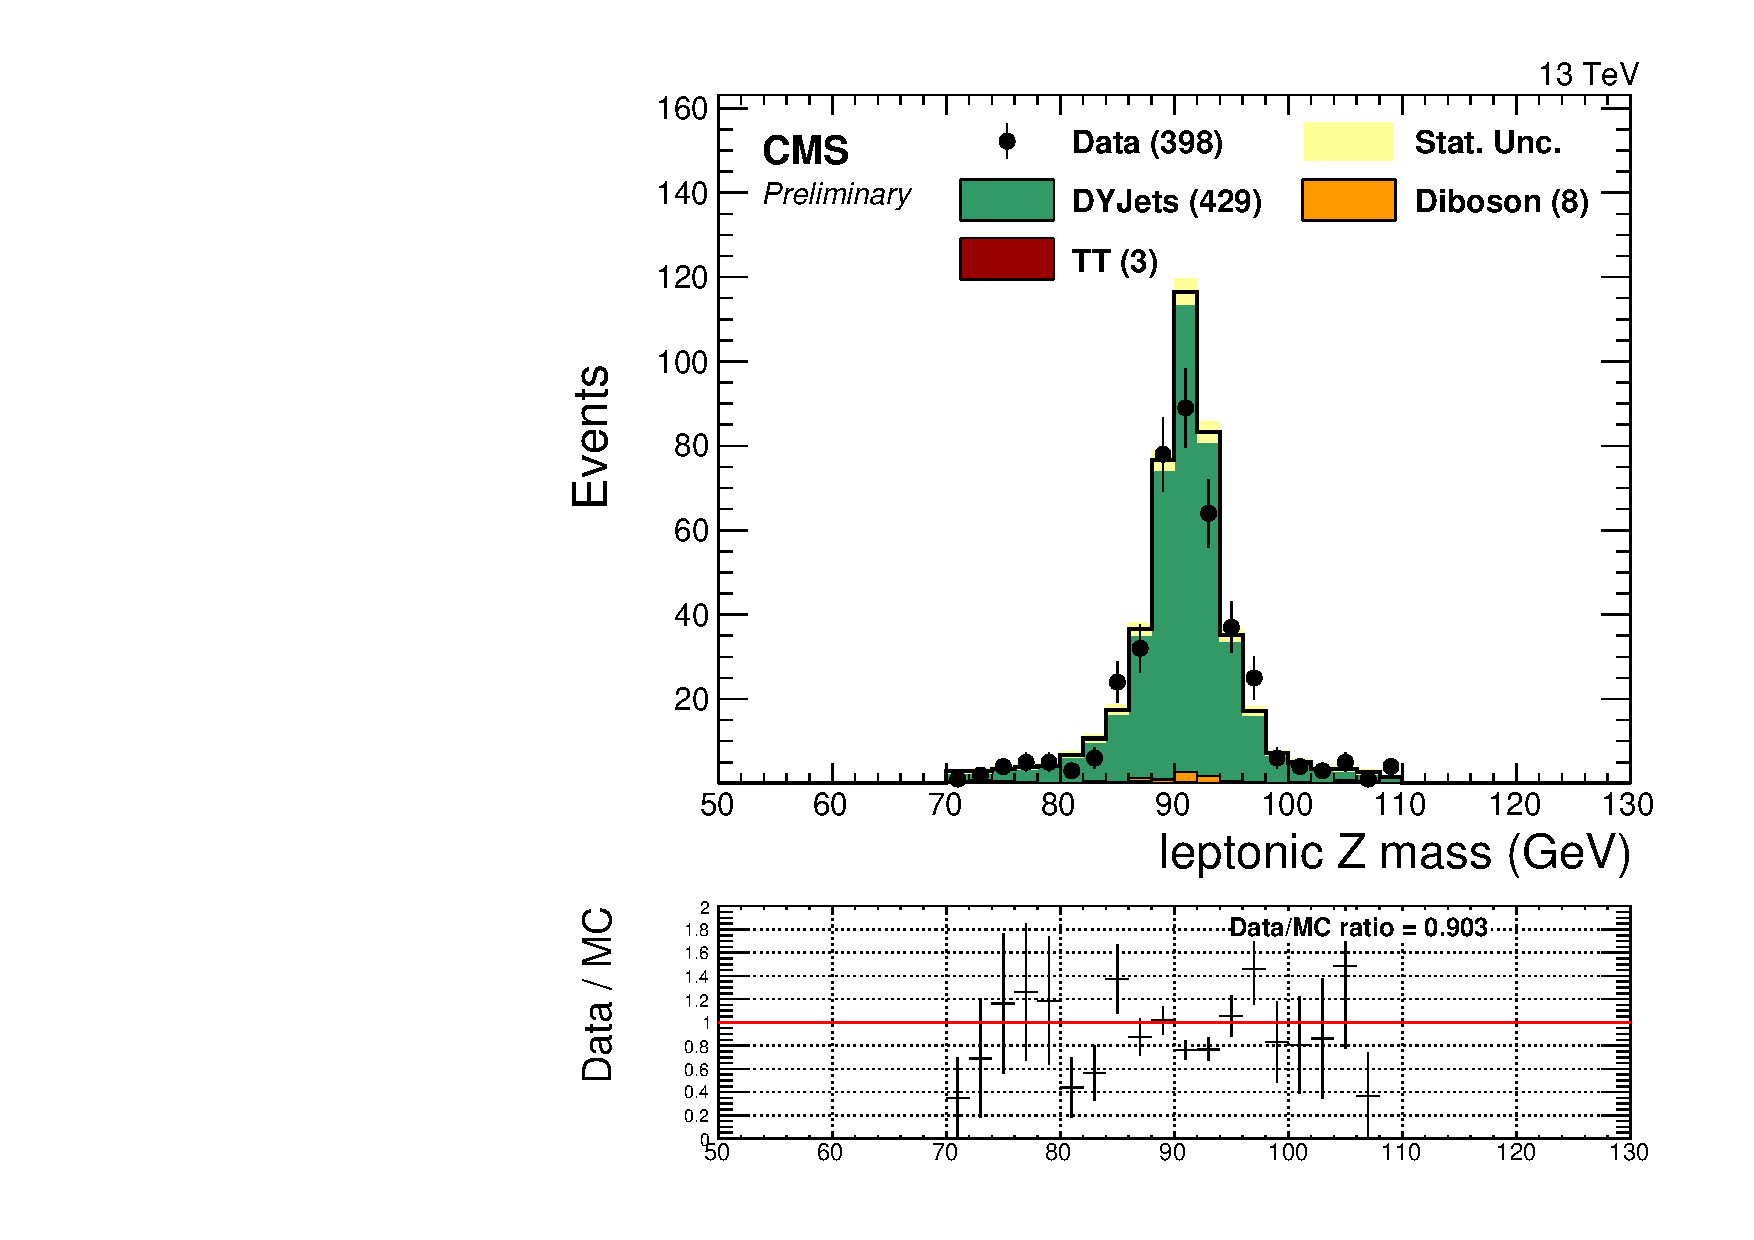
\includegraphics[scale=0.37]{figures/control/massZllMLP.pdf}
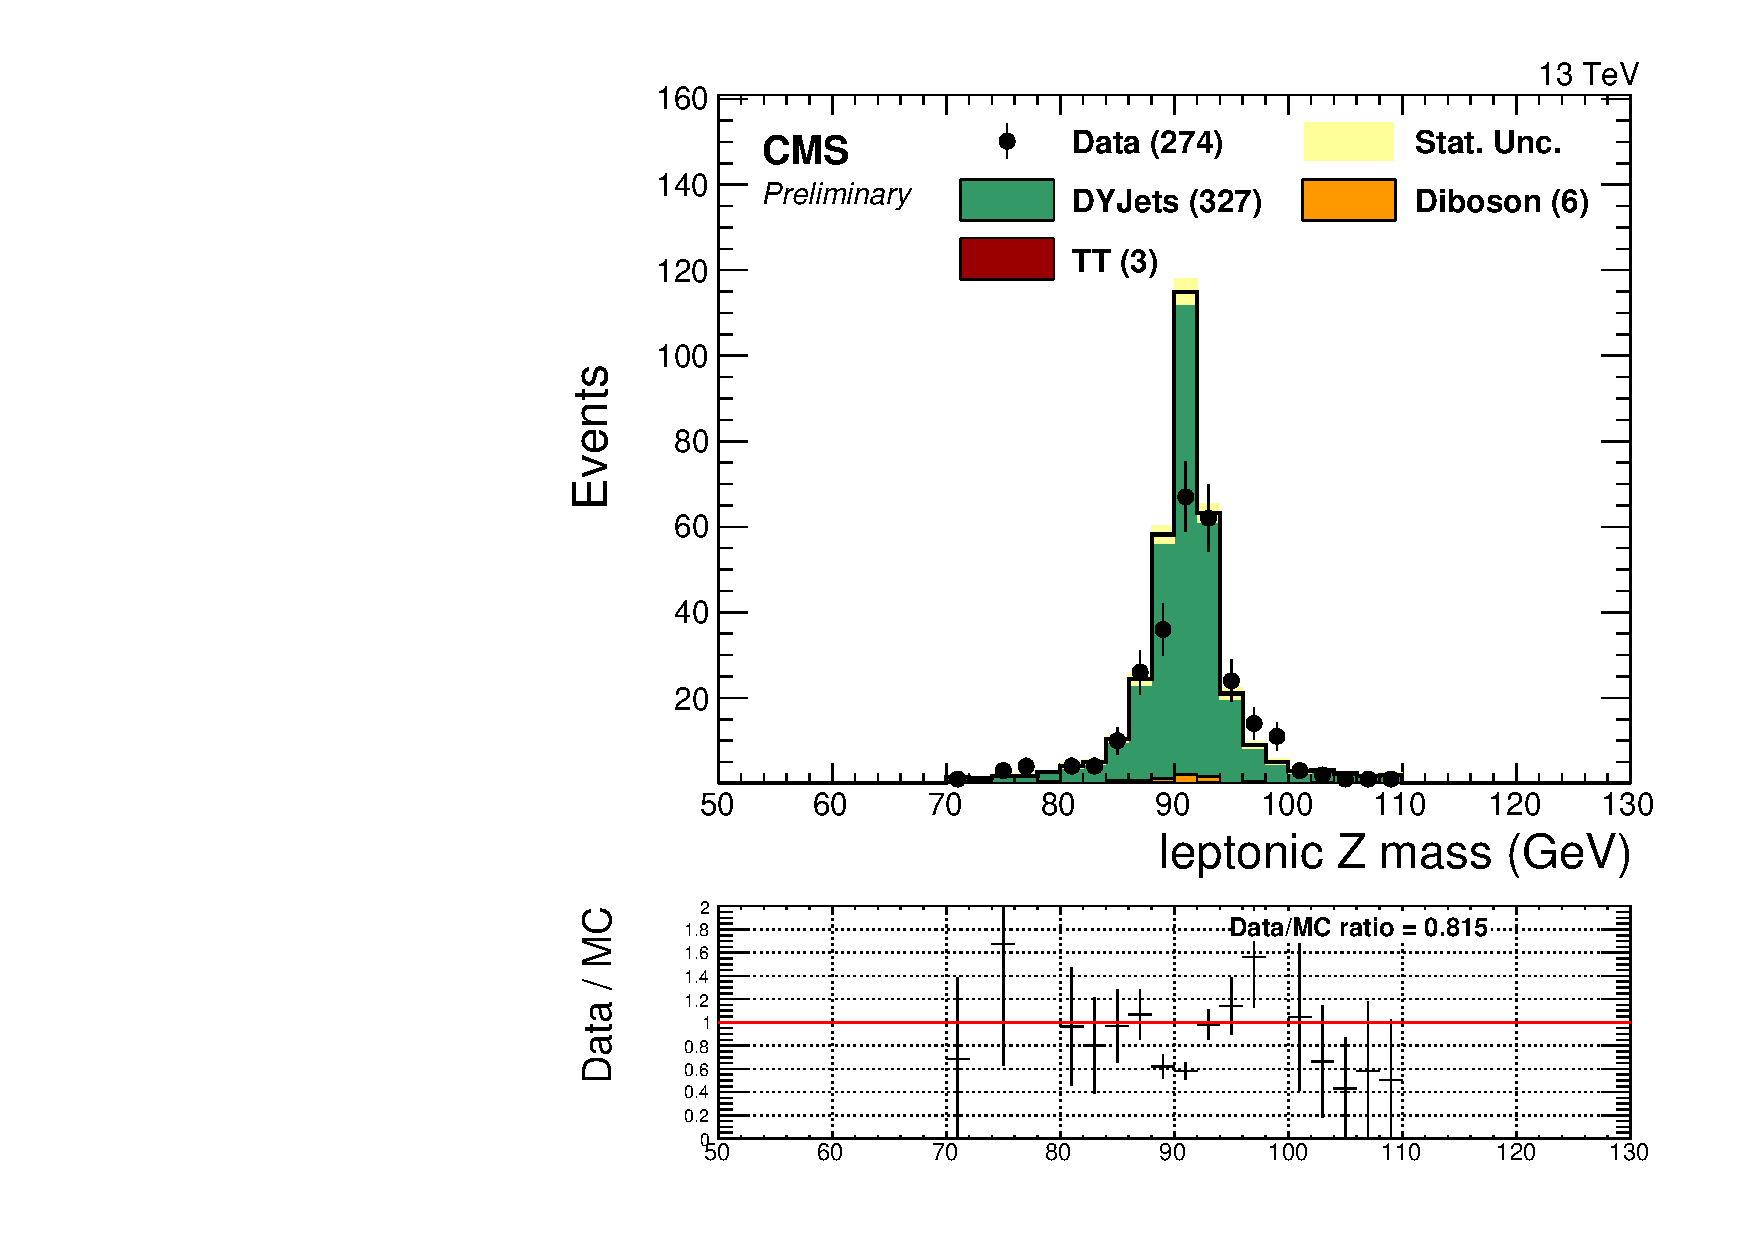
\includegraphics[scale=0.37]{figures/control/massZllELP.pdf}\\[2cm]
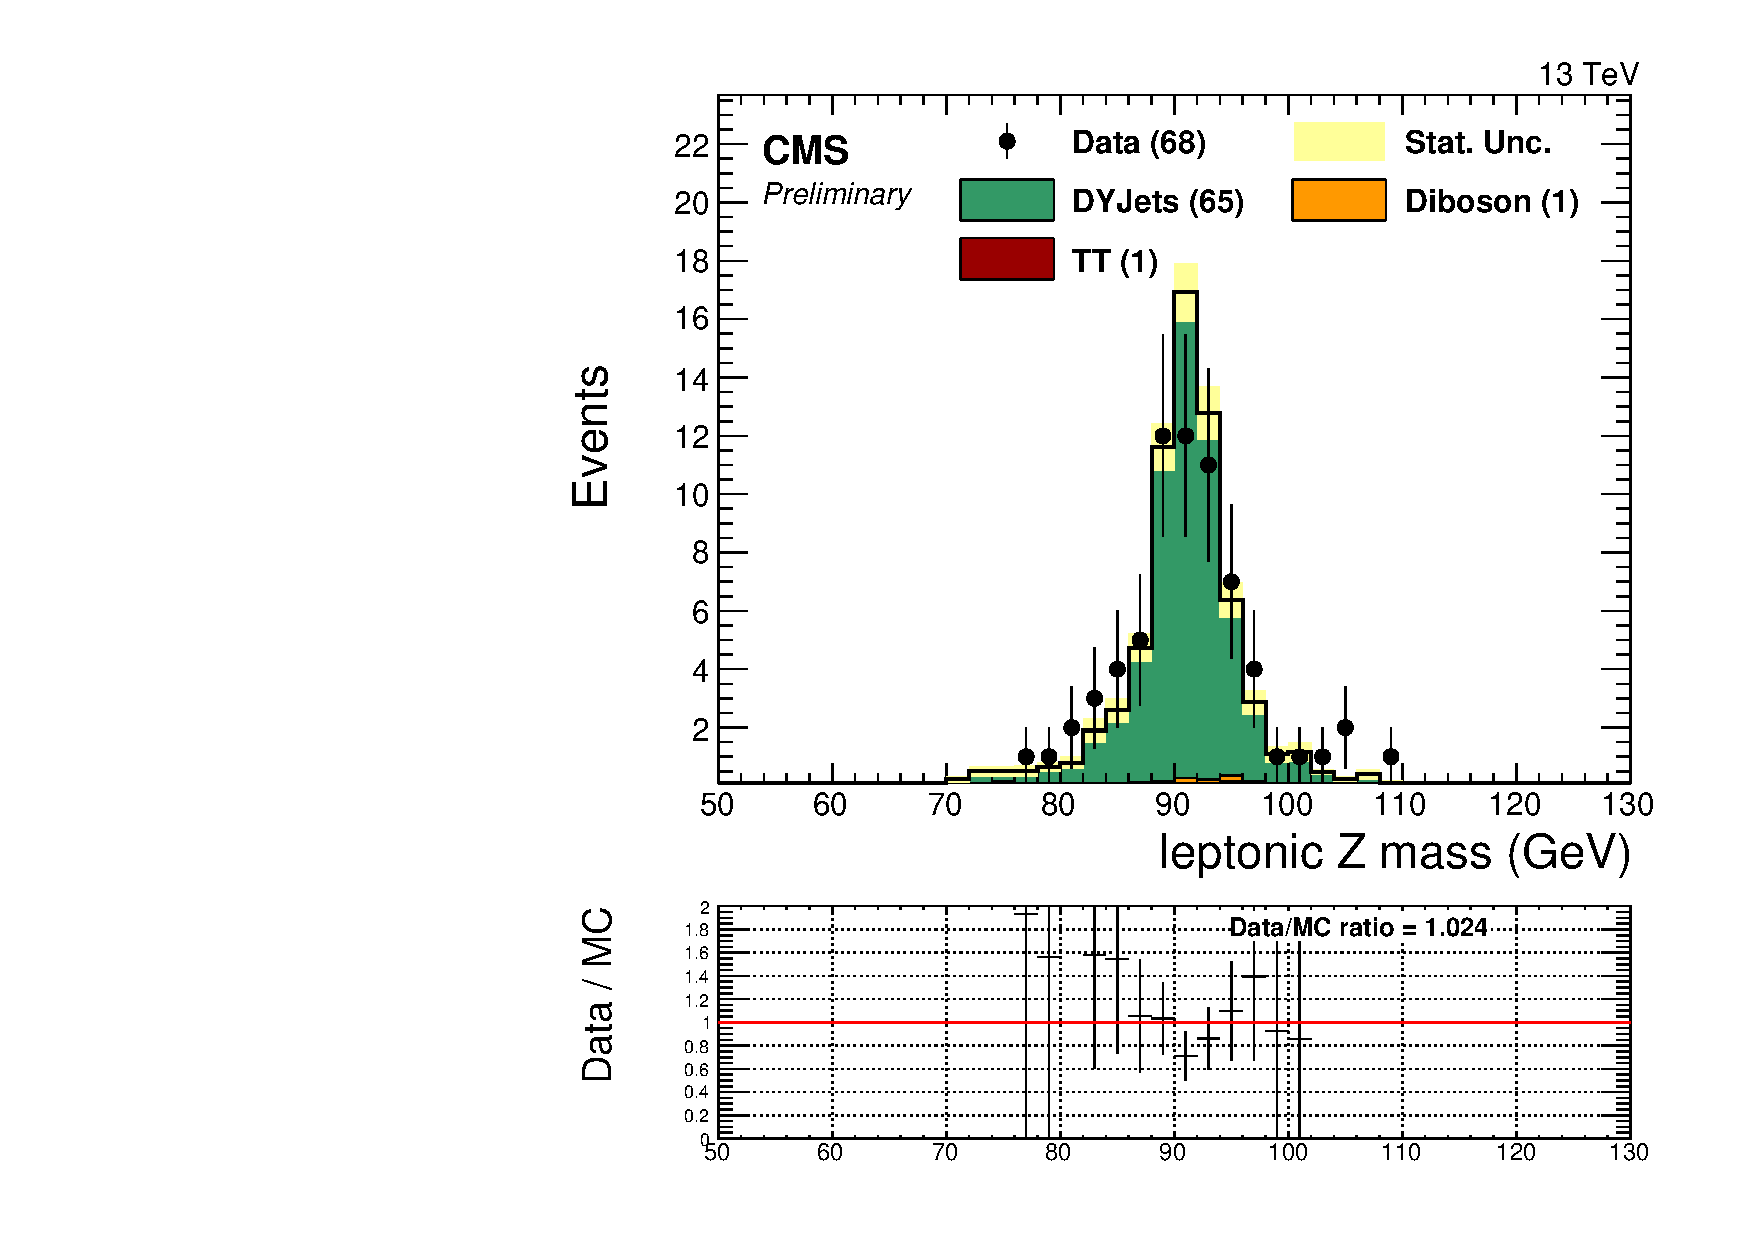
\includegraphics[scale=0.37]{figures/control/massZllMHP.pdf}
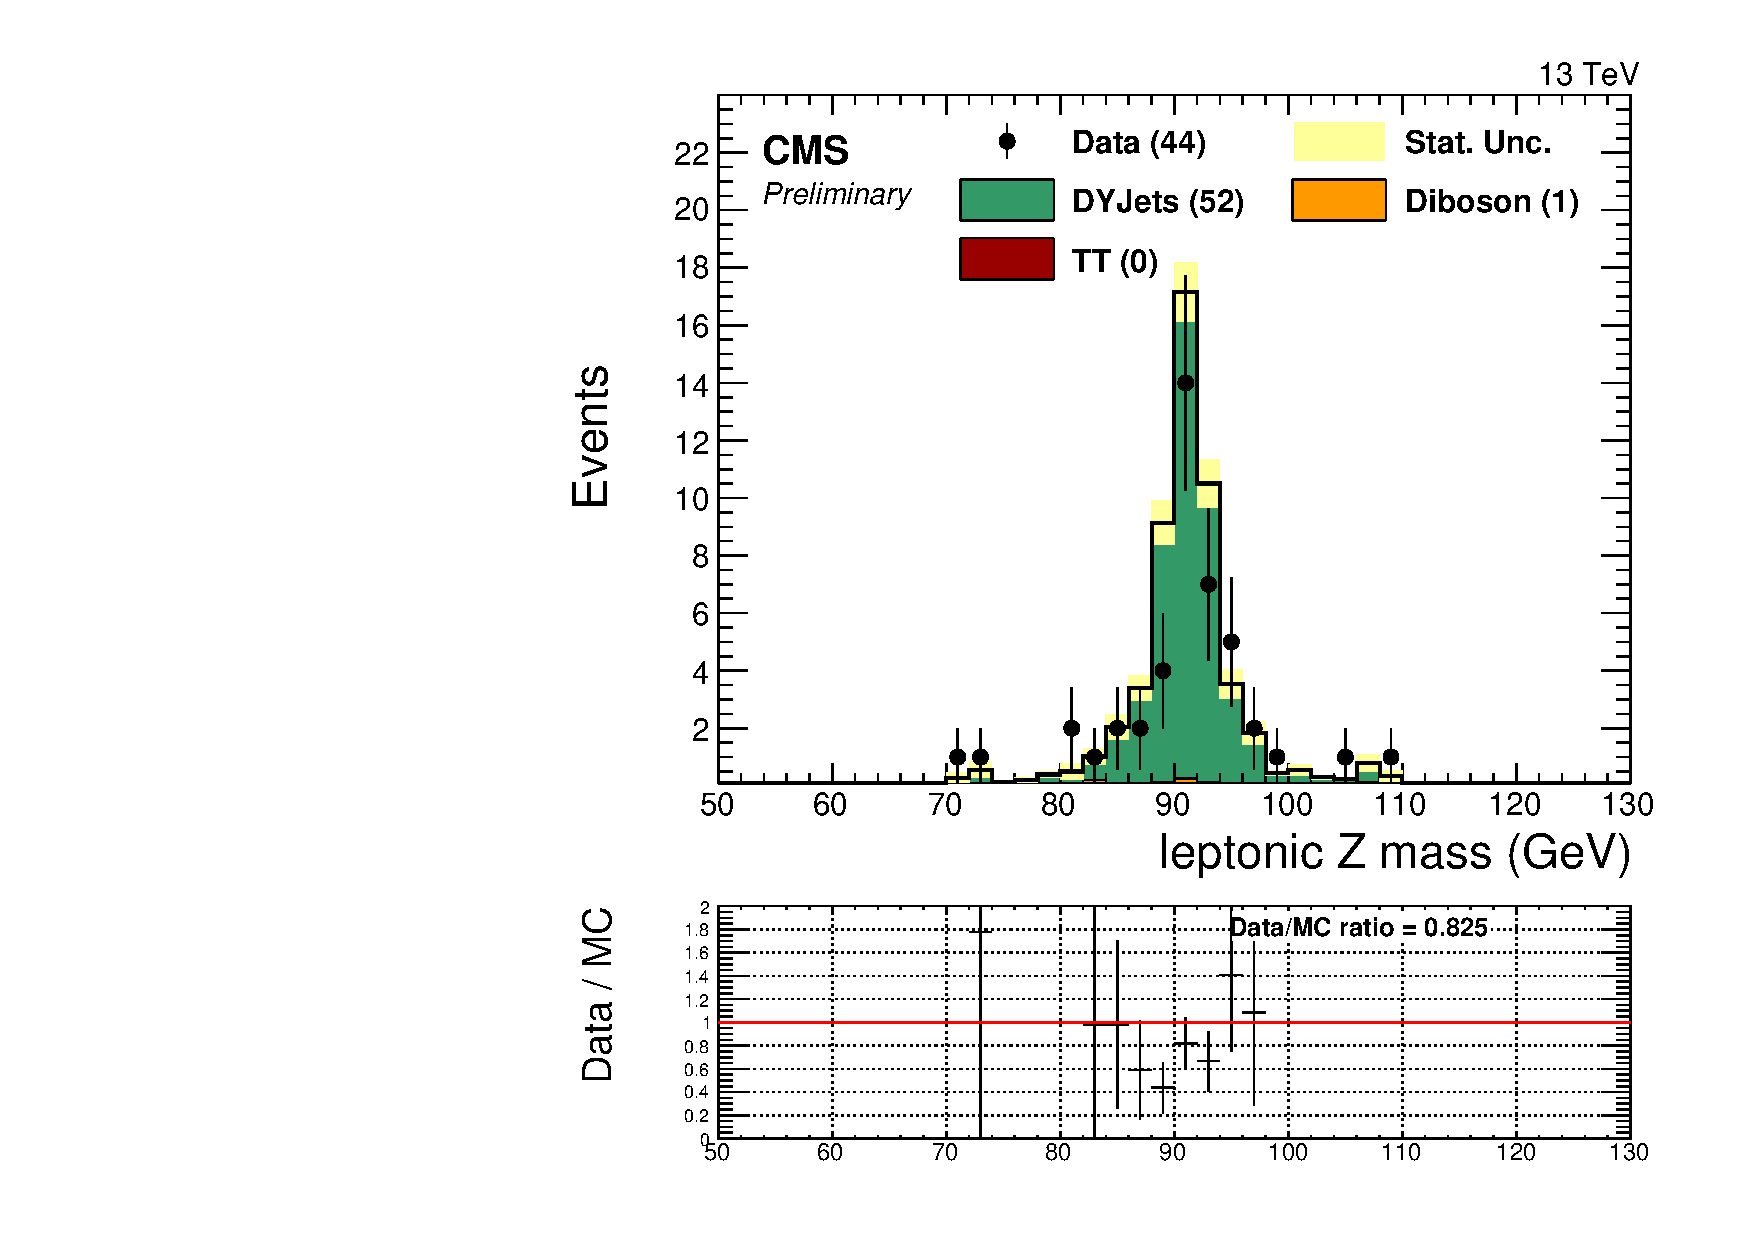
\includegraphics[scale=0.37]{figures/control/massZllEHP.pdf}
\caption[Distribution of mass of the leptonic Z candidate]{Distribution of mass of the leptonic Z candidate in the category: muon low purity (top-left), electron low purity (top-right), muon high purity (bottom-left), and  electron high purity (bottom-right). Simulated backgrounds are displayed as stacked histograms normalized to luminosity (2.7 fb$^{-1}$).}
\label{massZll_VZ}
\end{center}
\end{figure}
\begin{figure}[h]
\begin{center}
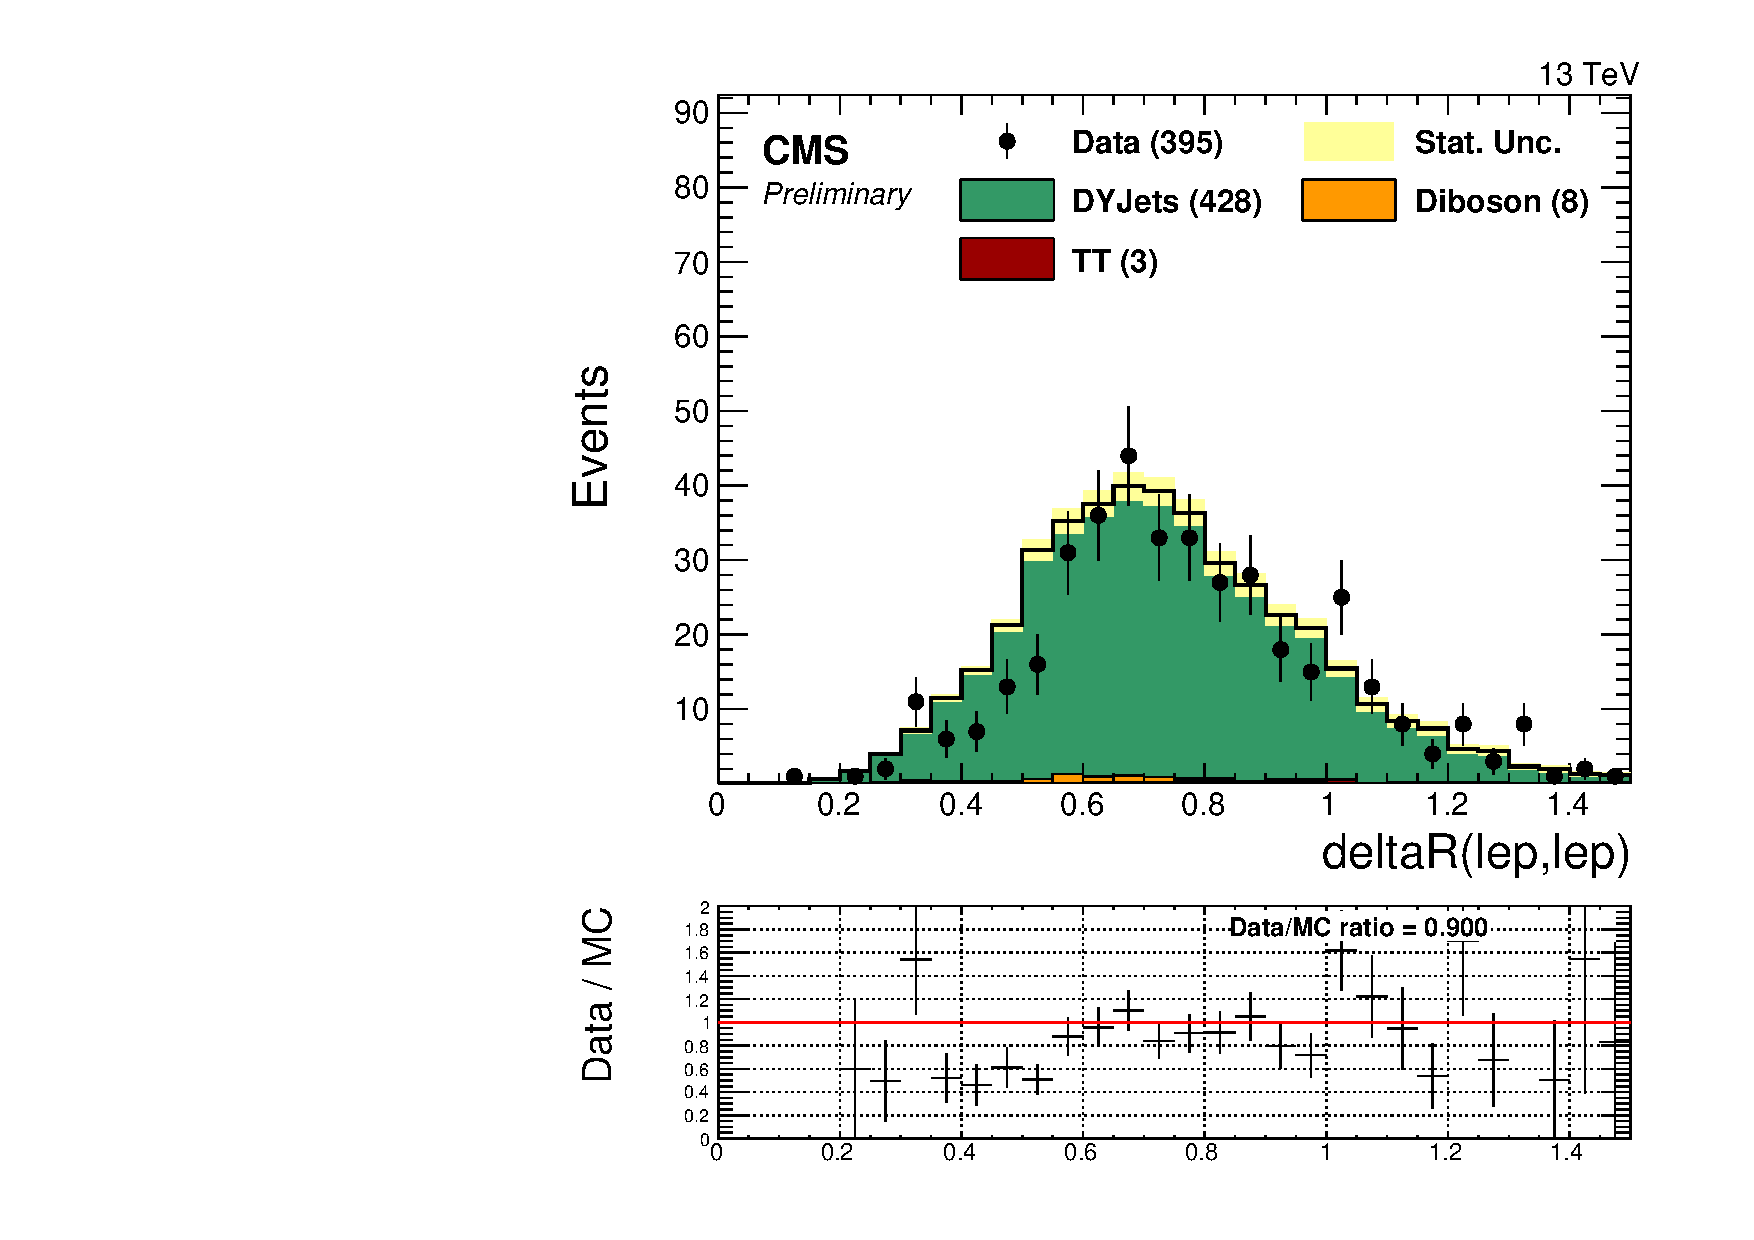
\includegraphics[scale=0.37]{figures/control/deltaRleplepMLP.pdf}
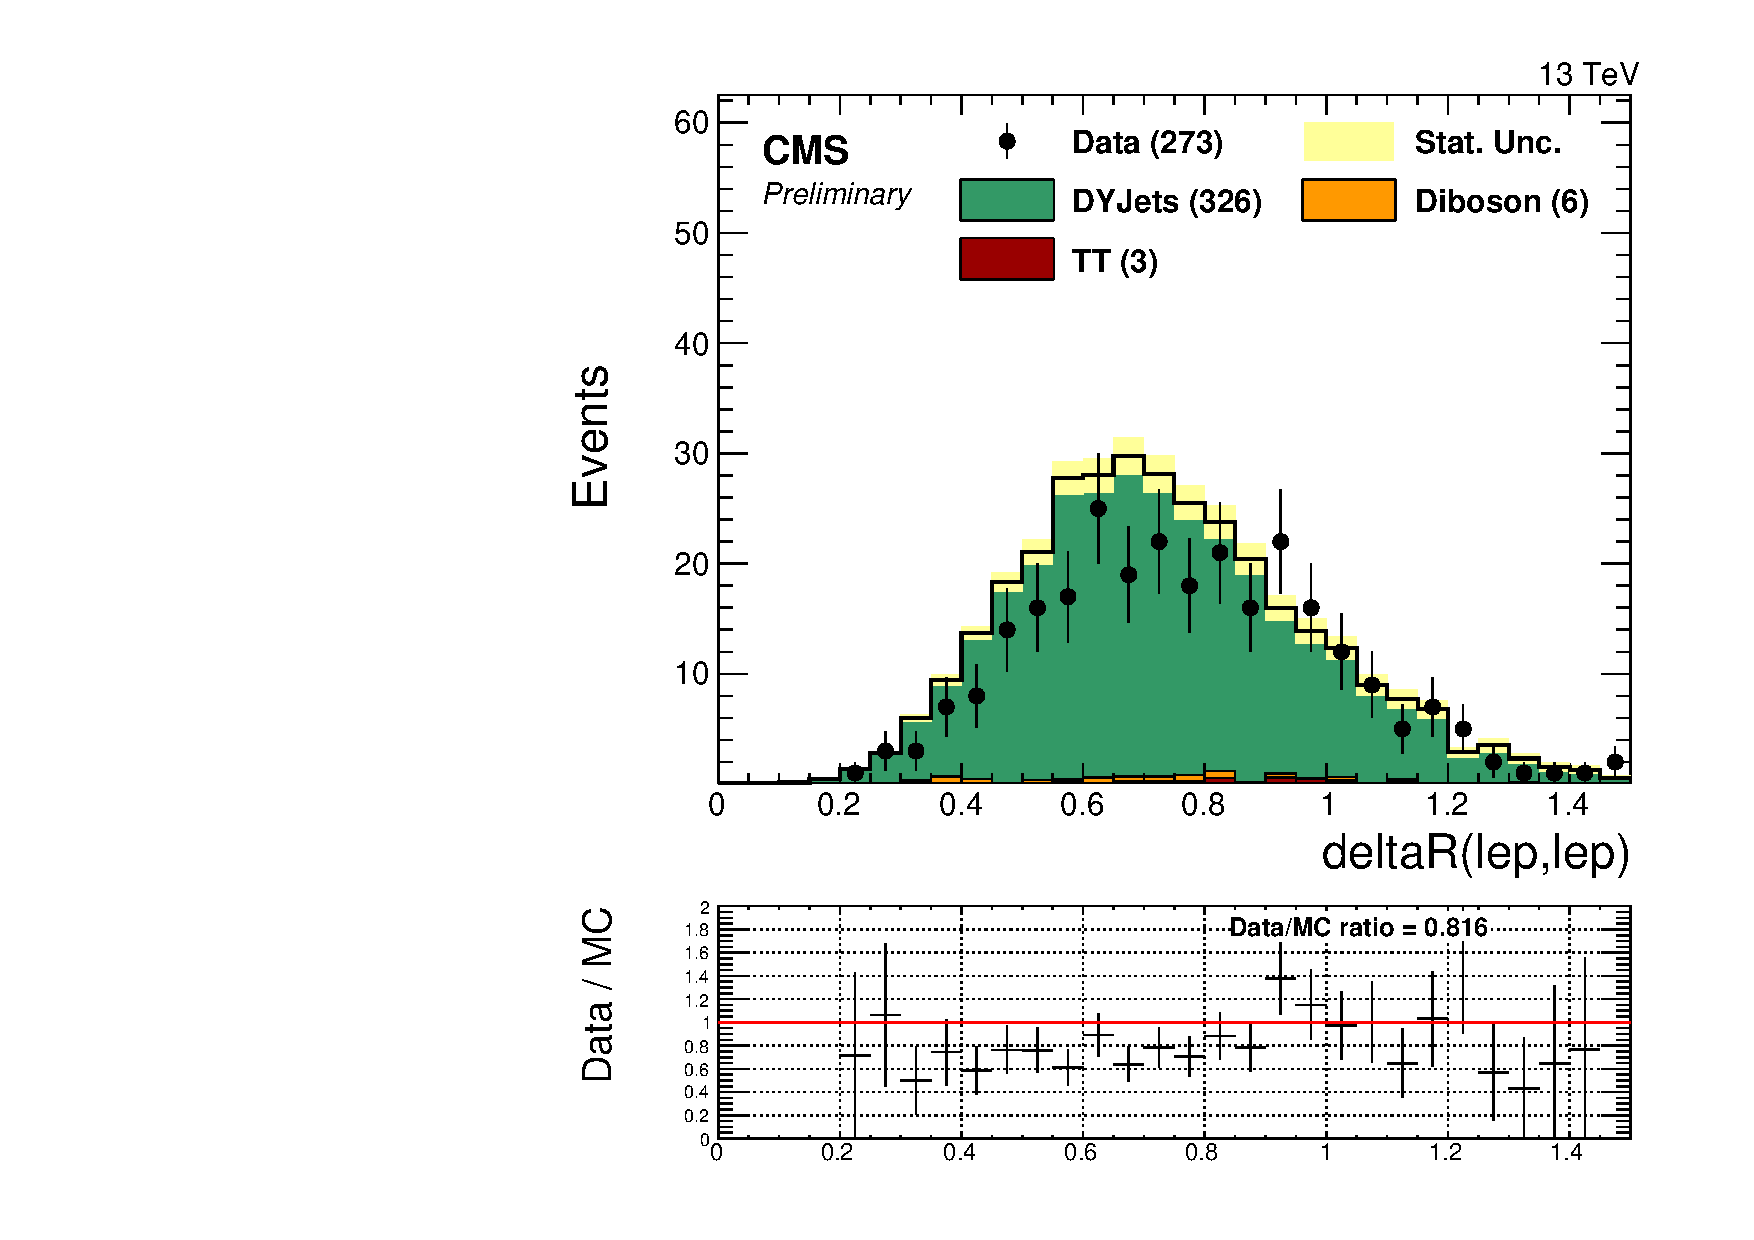
\includegraphics[scale=0.37]{figures/control/deltaRleplepELP.pdf}\\[2cm]
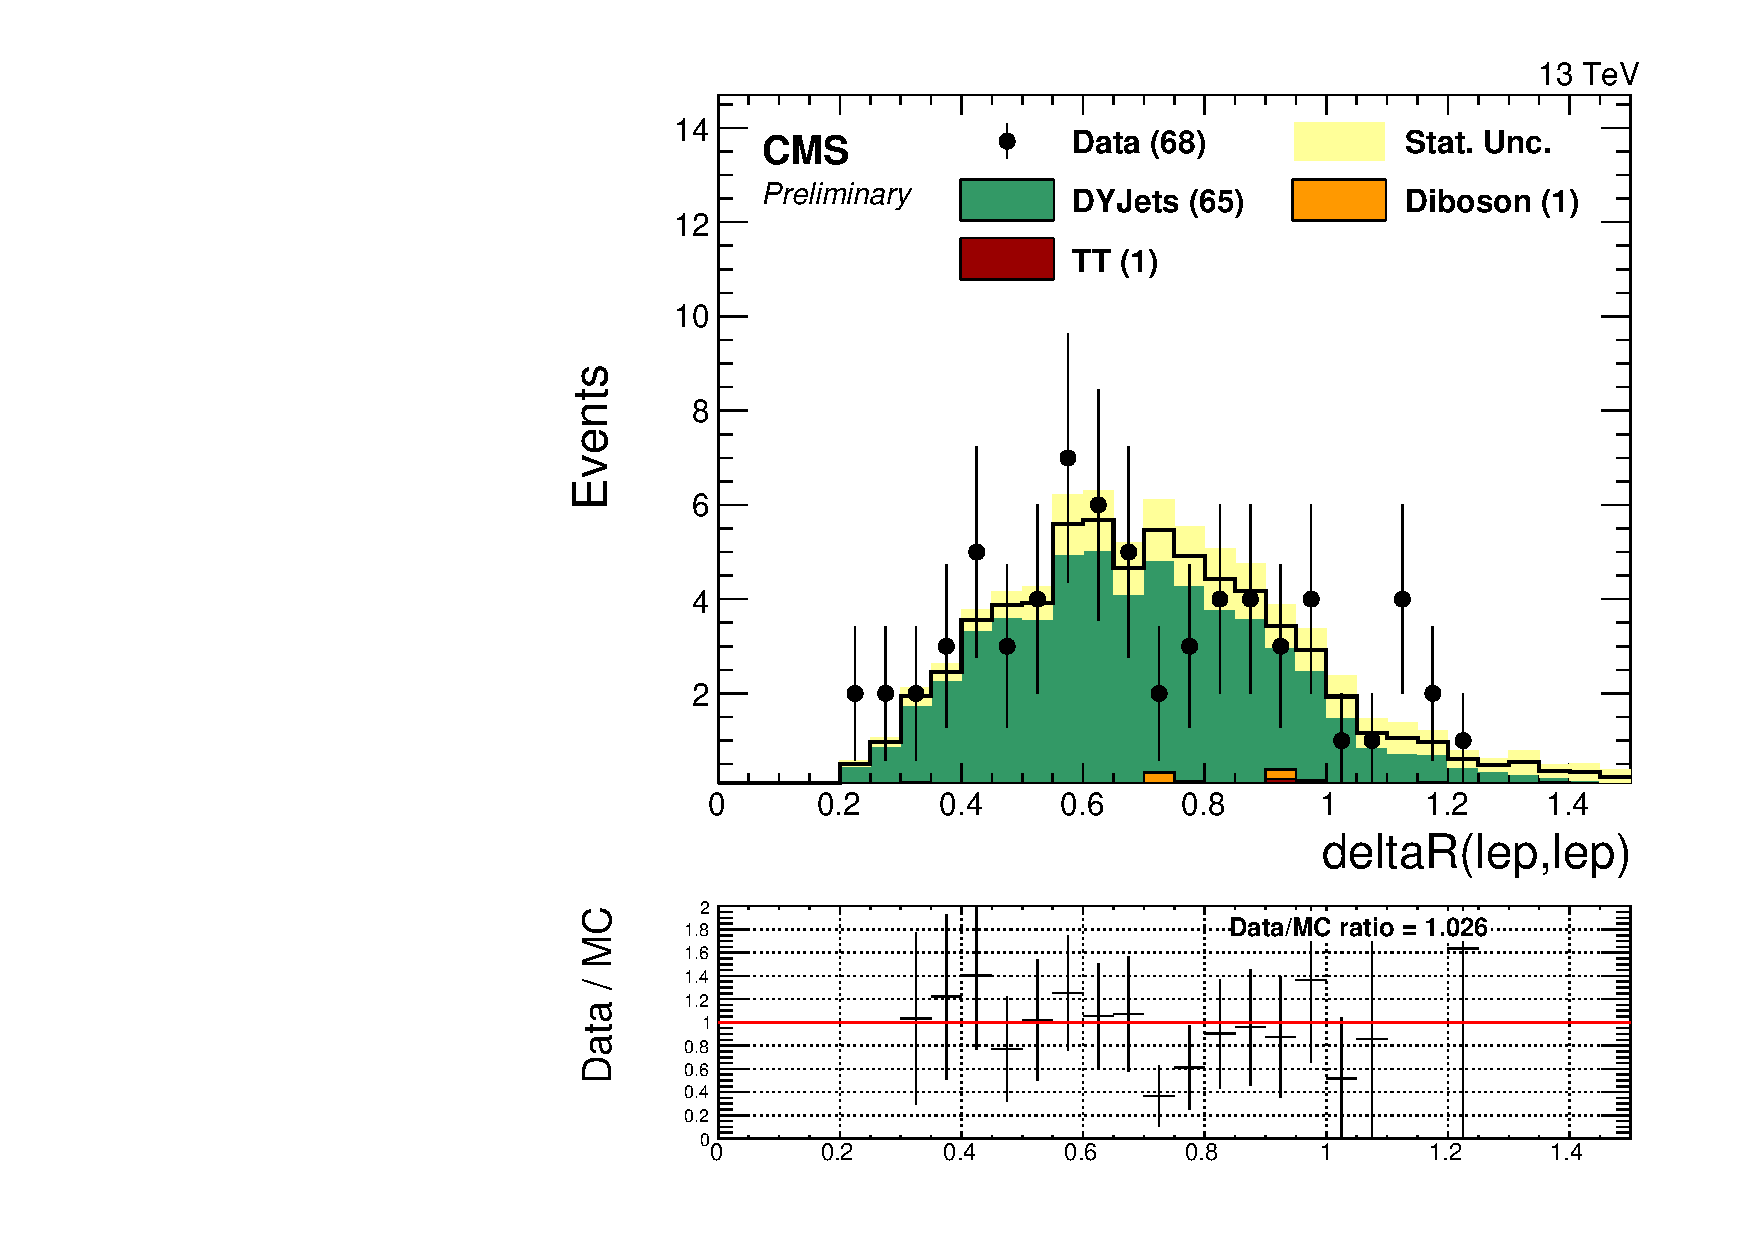
\includegraphics[scale=0.37]{figures/control/deltaRleplepMHP.pdf}
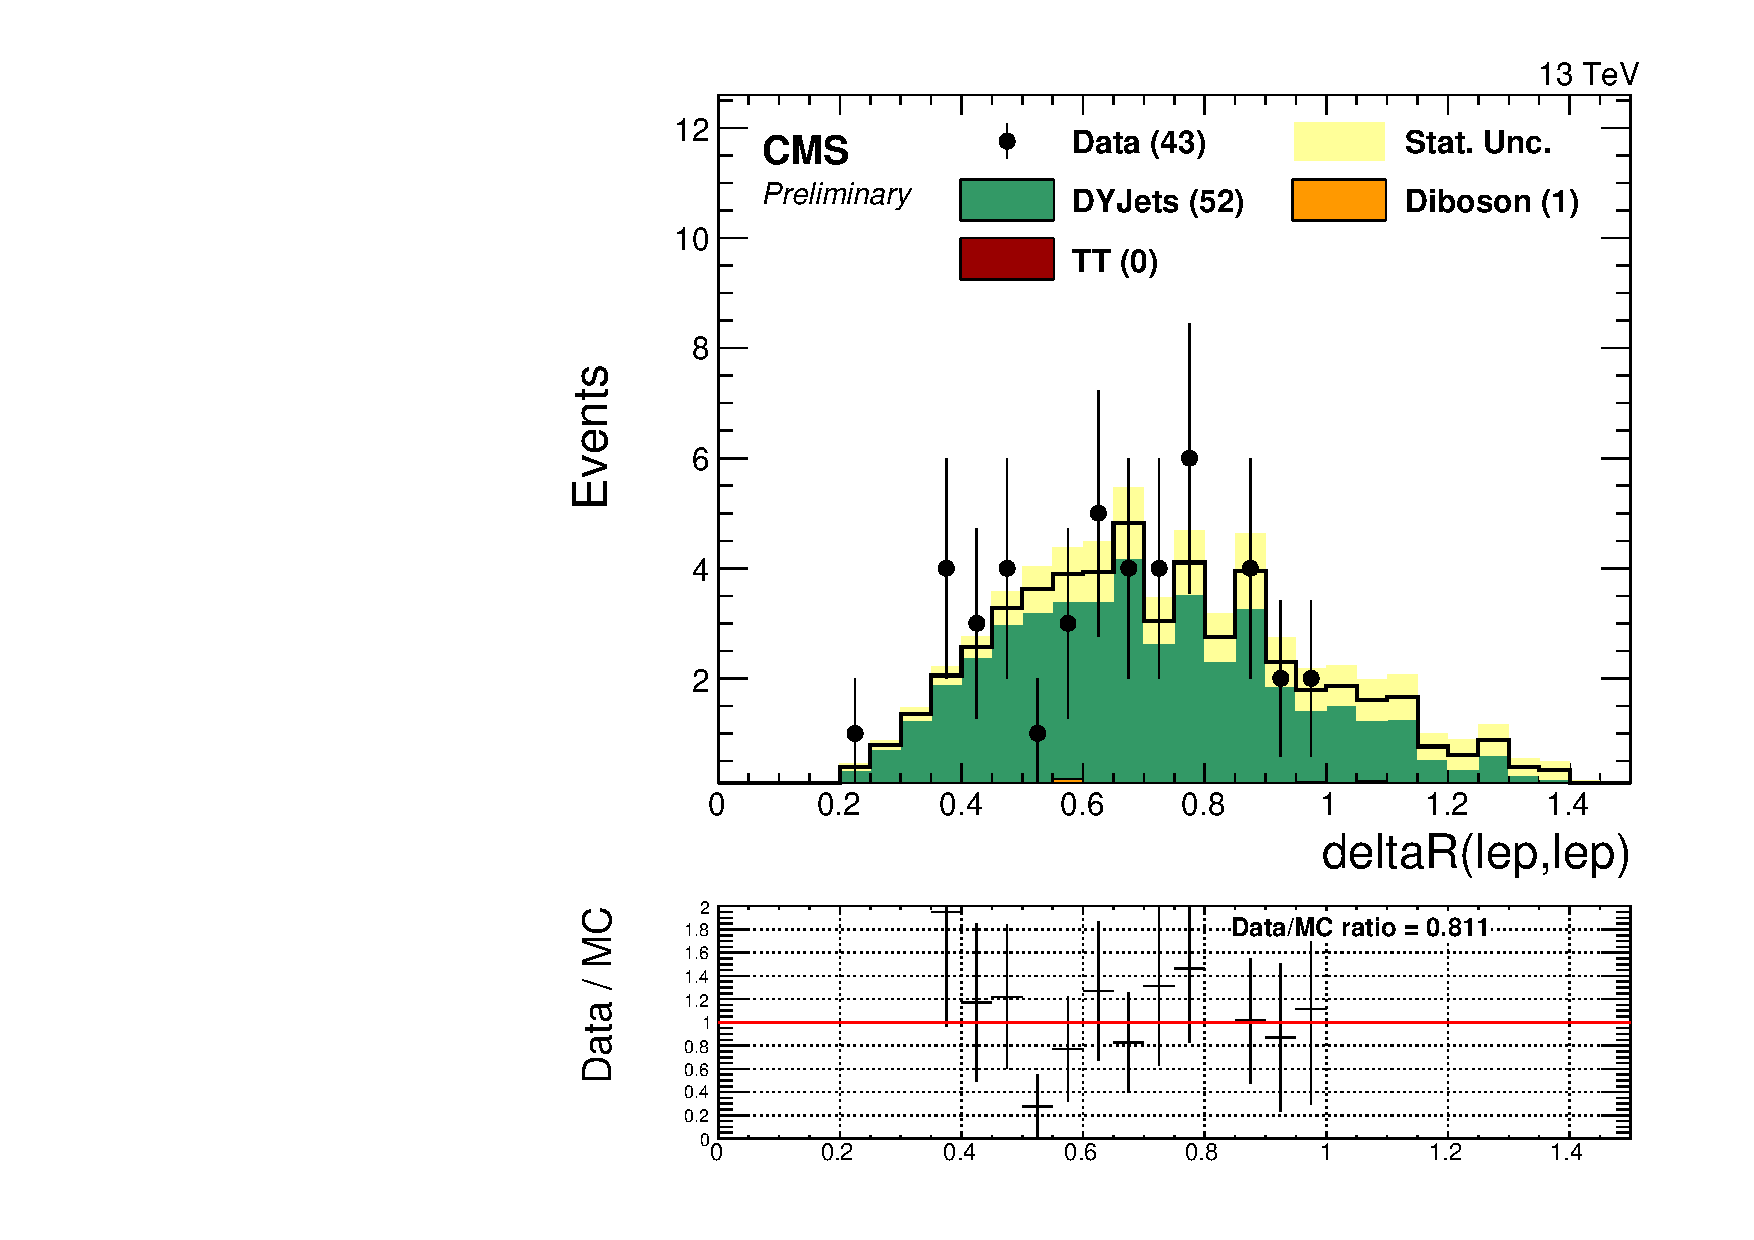
\includegraphics[scale=0.37]{figures/control/deltaRleplepEHP.pdf}
\caption[Distribution of $\Delta R$ between leptons]{Distribution of $\Delta R$ between leptons in the category: muon low purity (top-left), electron low purity (top-right), muon high purity (bottom-left), and  electron high purity (bottom-right). Simulated backgrounds are displayed as stacked histograms normalized to luminosity (2.7 fb$^{-1}$).}
\label{deltaRleplep_VZ}
\end{center}
\end{figure}

\begin{figure}[h]
\begin{center}
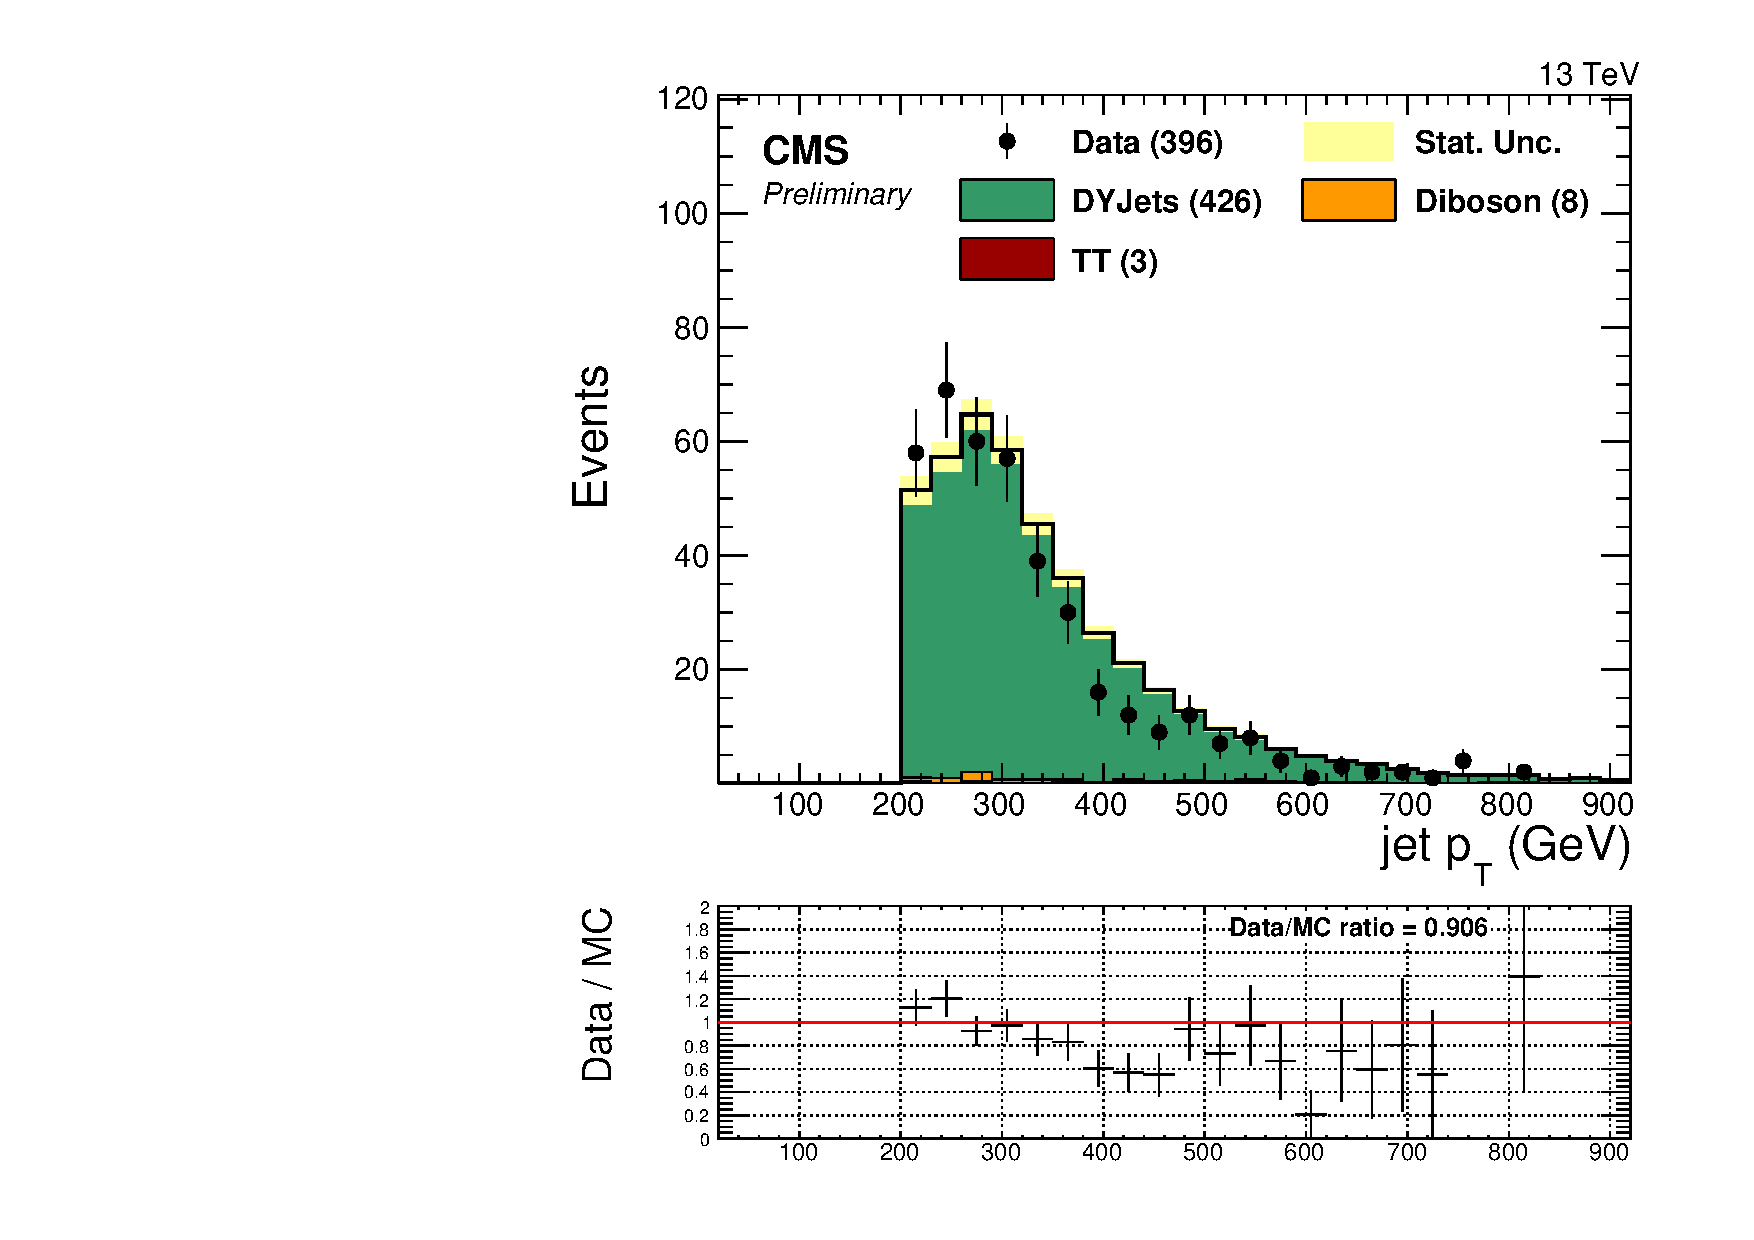
\includegraphics[scale=0.37]{figures/control/ptZjjMLP.pdf}
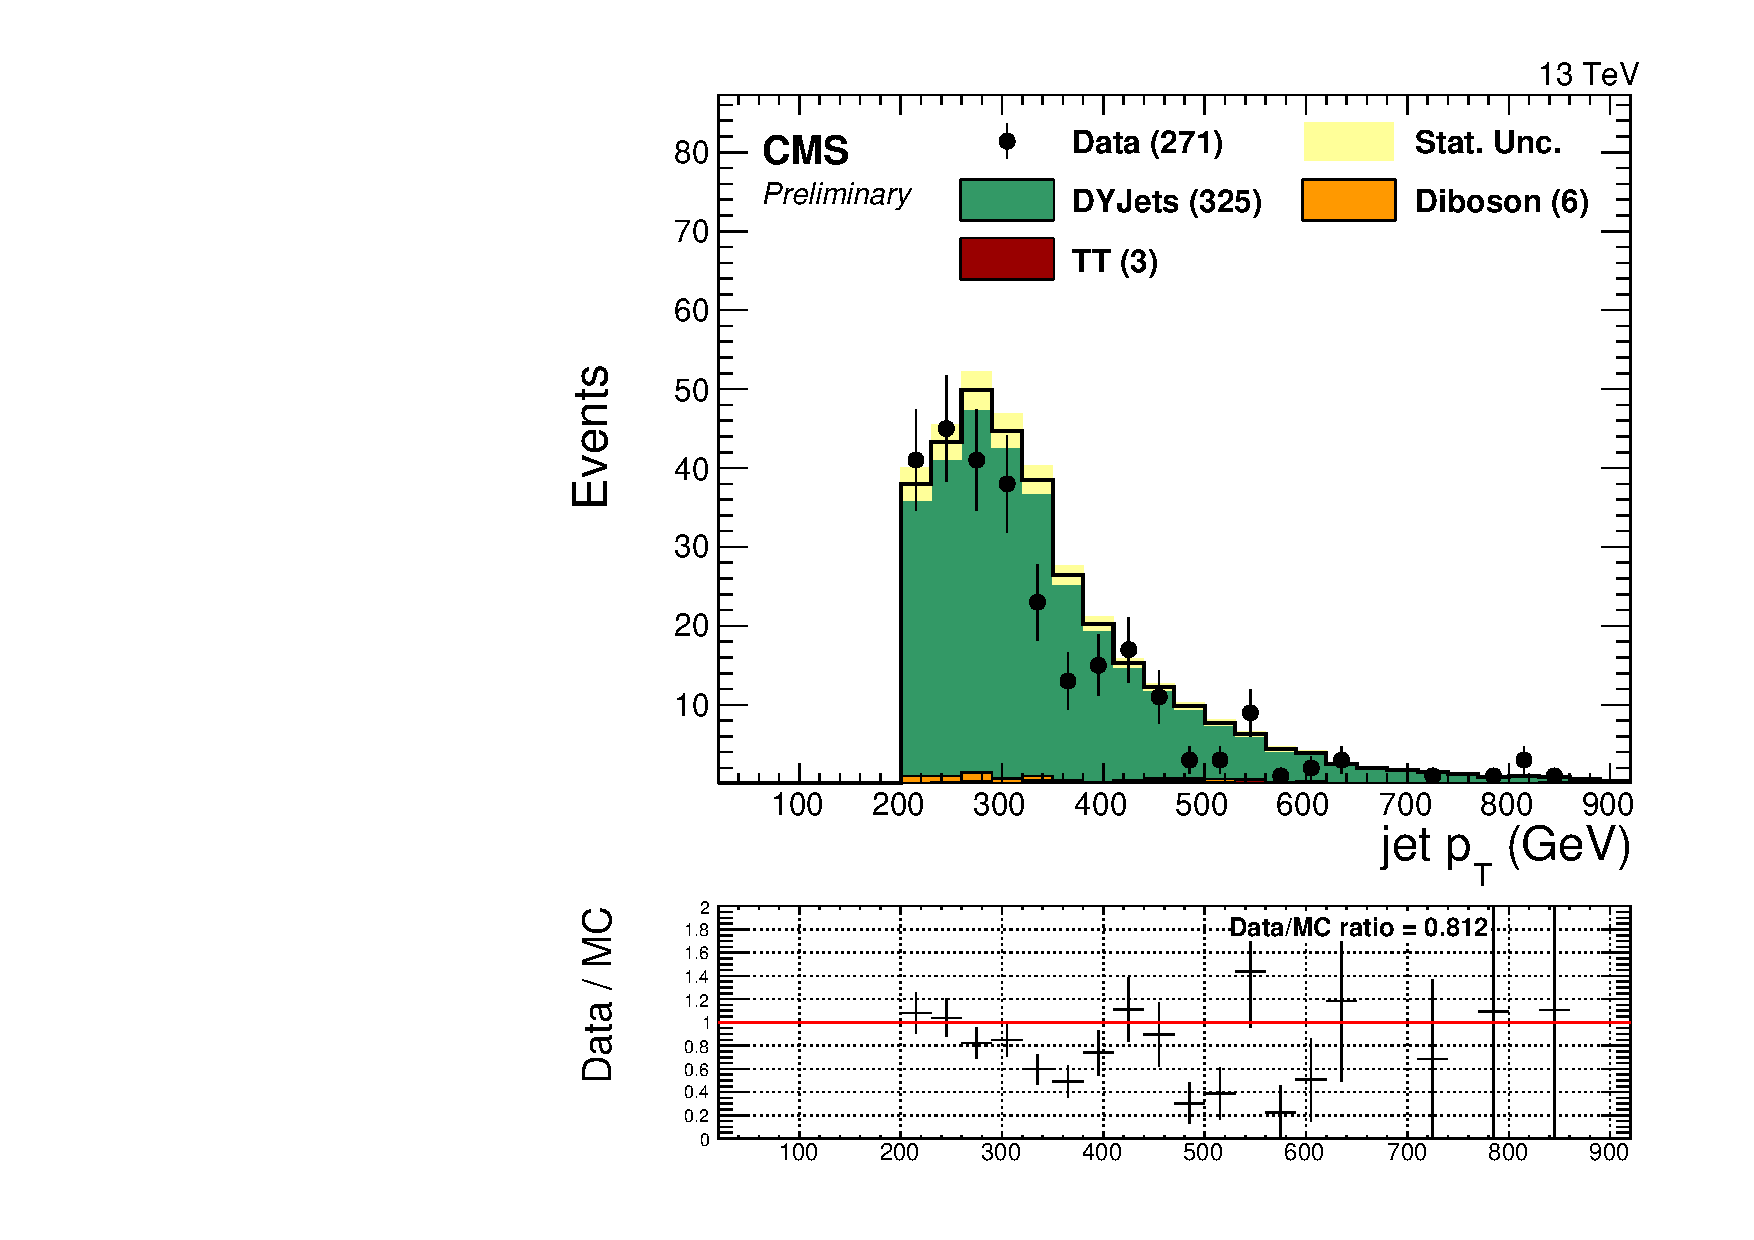
\includegraphics[scale=0.37]{figures/control/ptZjjELP.pdf}\\[2cm]
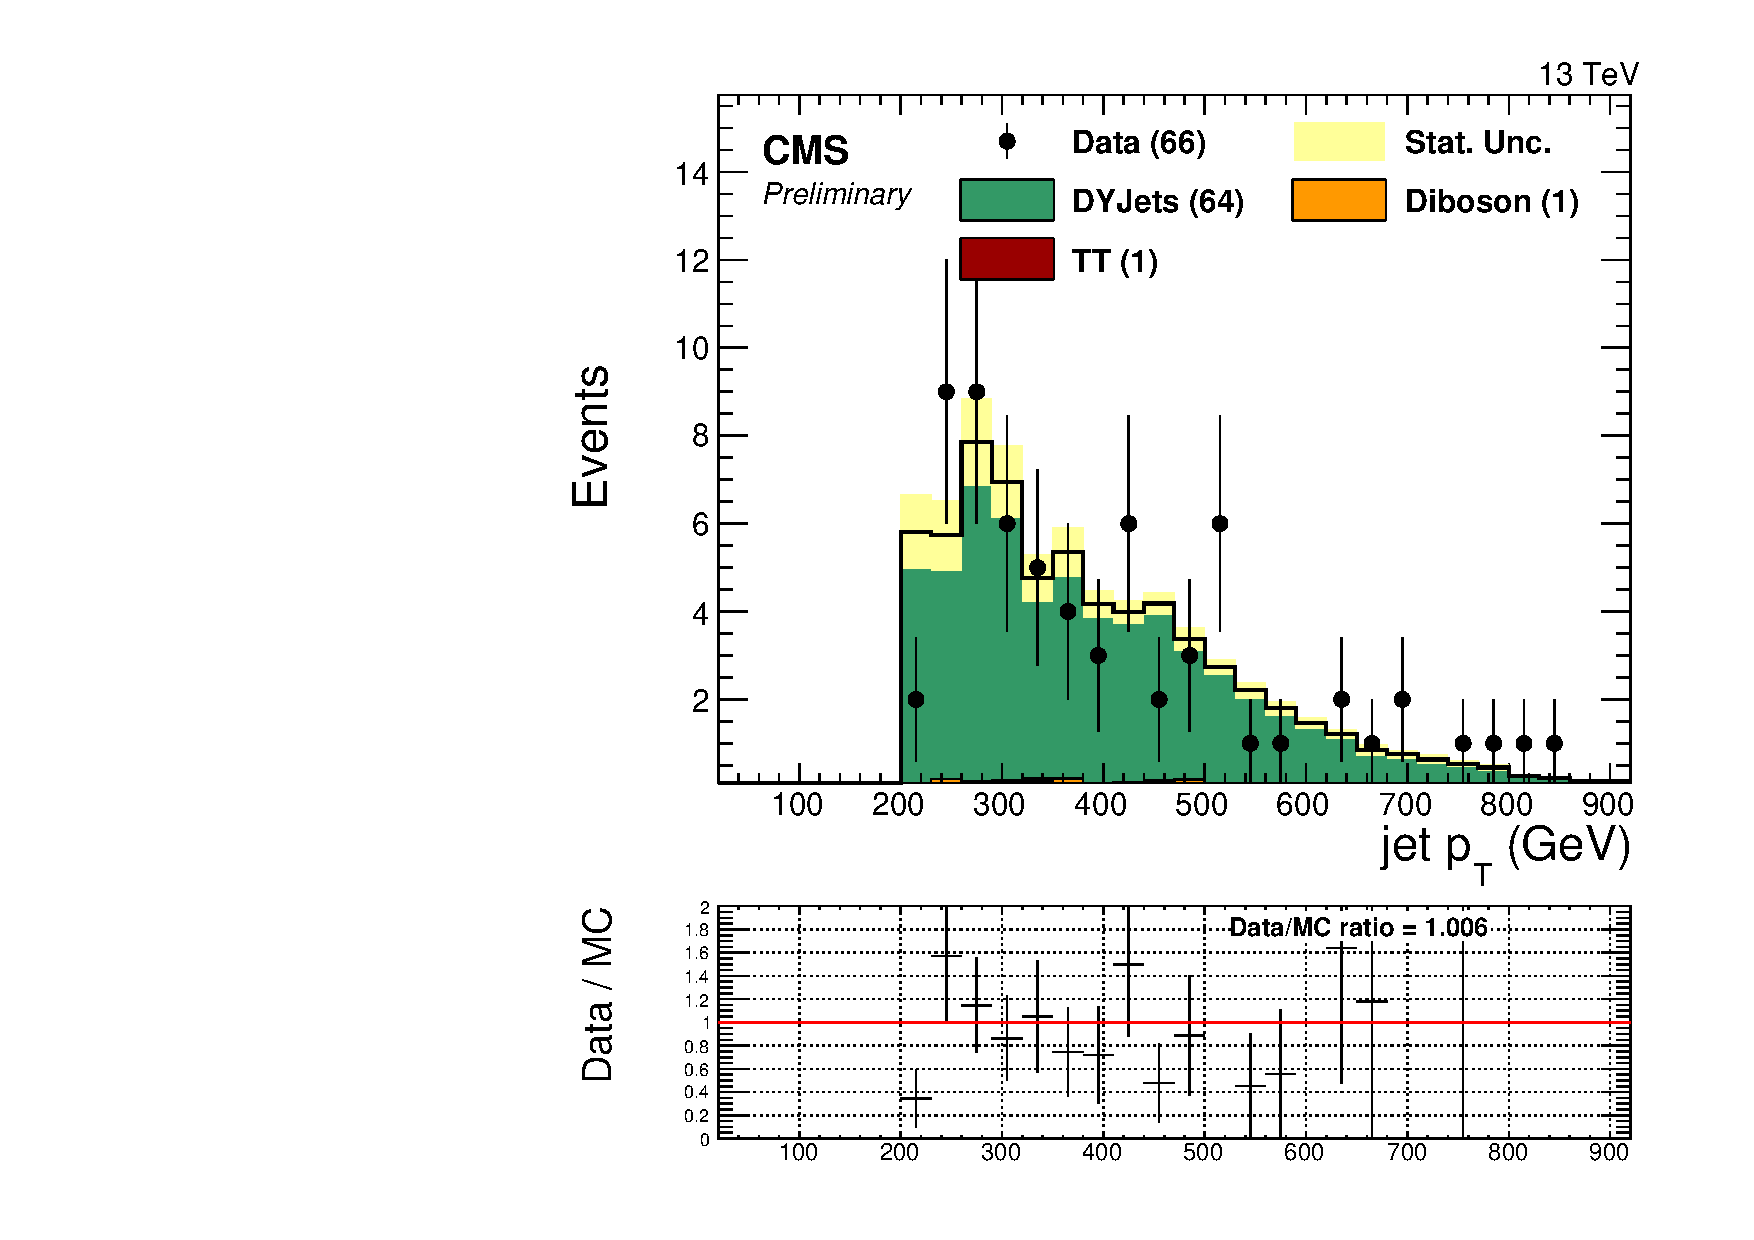
\includegraphics[scale=0.37]{figures/control/ptZjjMHP.pdf}
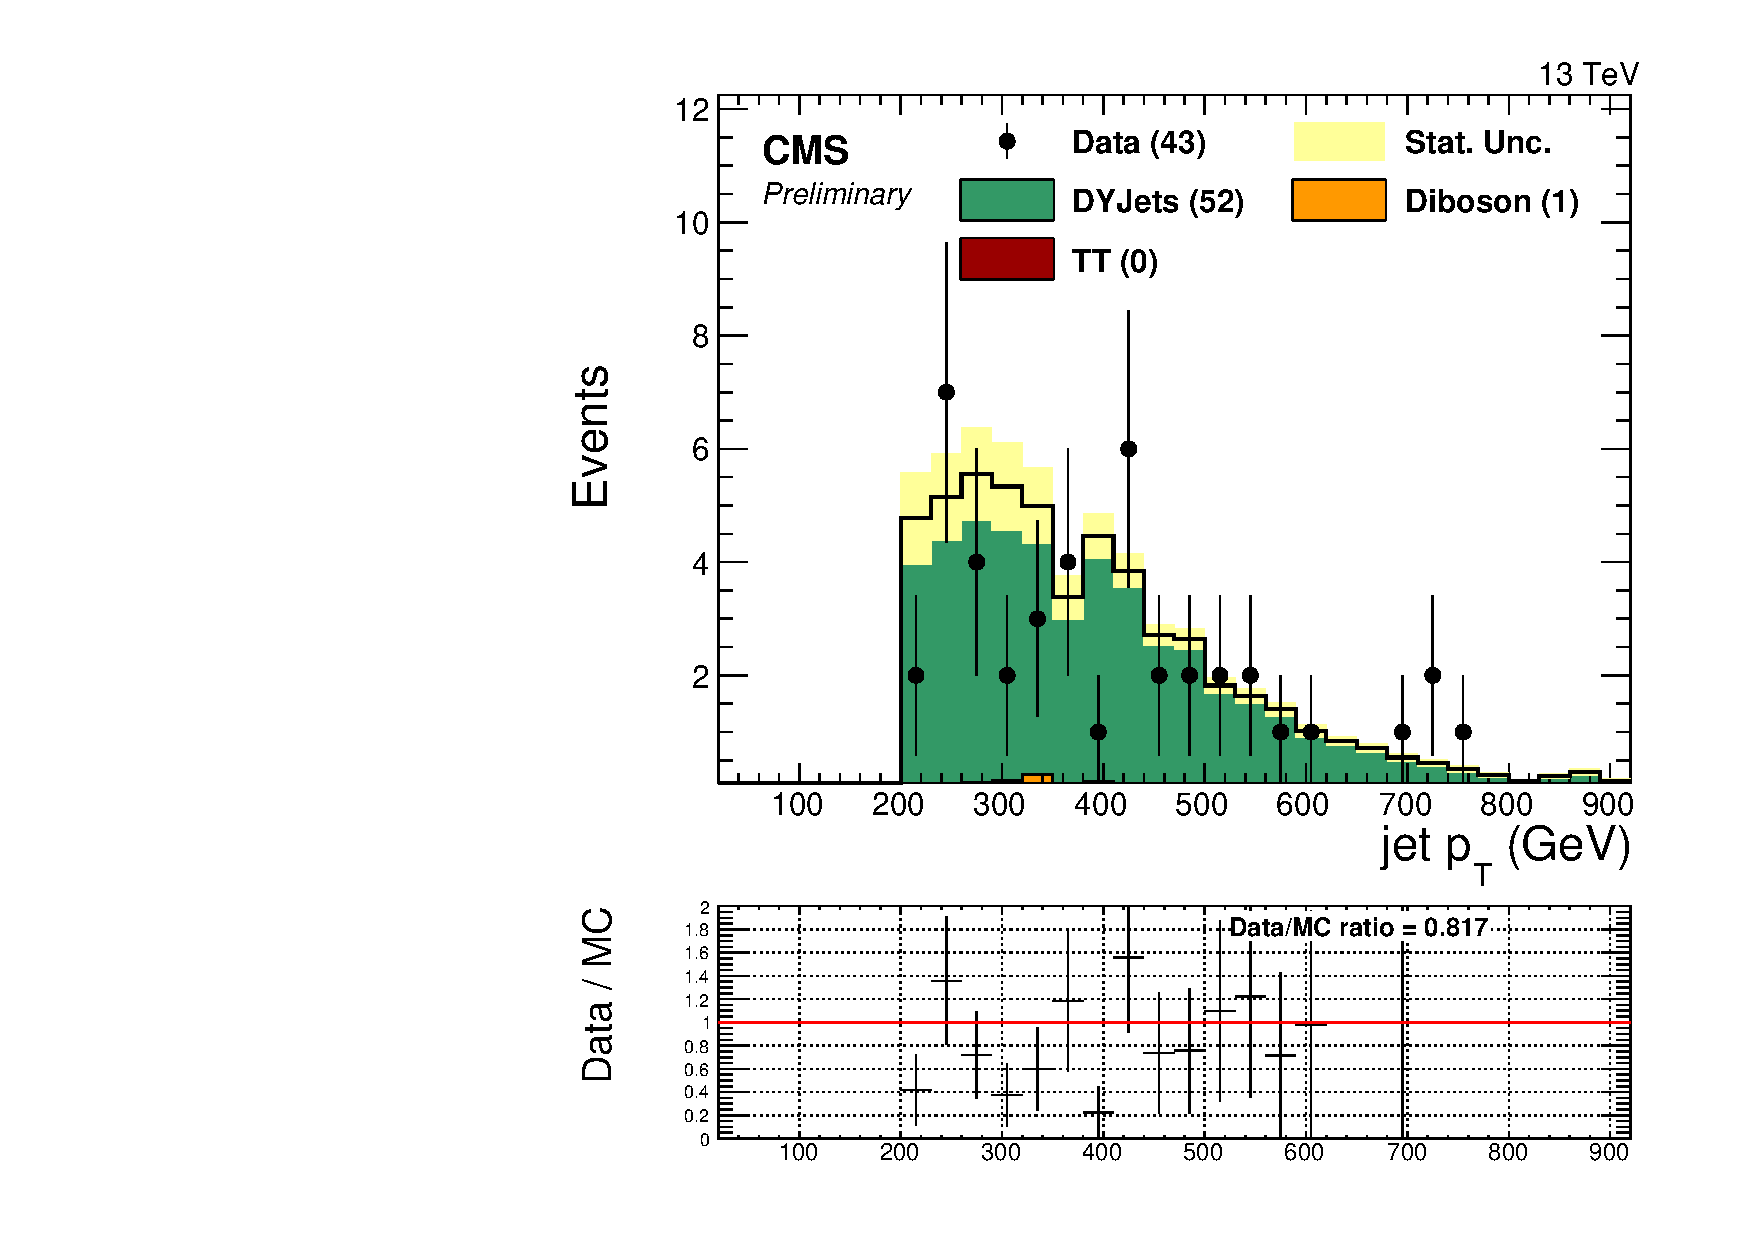
\includegraphics[scale=0.37]{figures/control/ptZjjEHP.pdf}
\caption[Distribution of jet \ptrans]{Distribution of jet \ptrans in the category: muon low purity (top-left), electron low purity (top-right), muon high purity (bottom-left), and  electron high purity (bottom-right). Simulated backgrounds are displayed as stacked histograms normalized to luminosity (2.7 fb$^{-1}$).}
\label{ptZjj_VZ}
\end{center}
\end{figure}
\begin{figure}[h]
\begin{center}
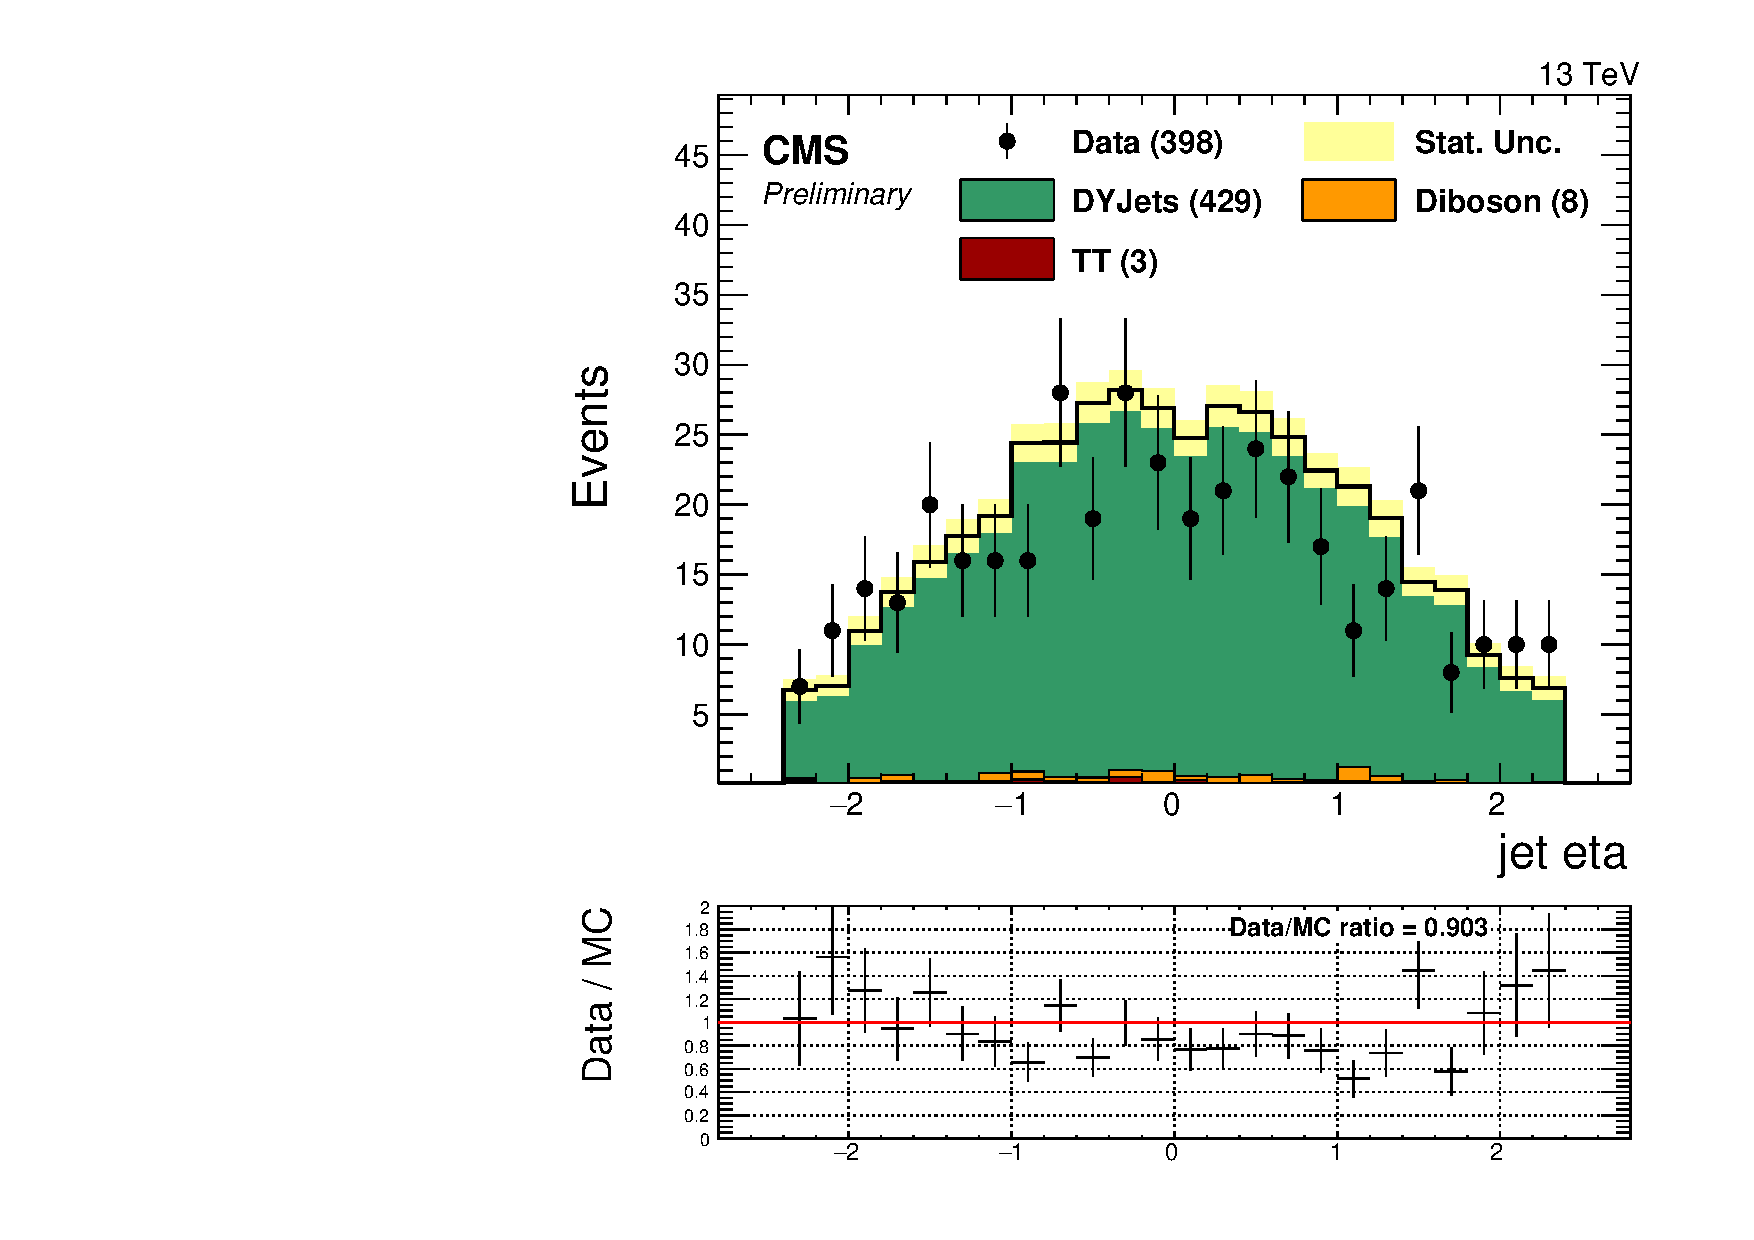
\includegraphics[scale=0.37]{figures/control/etaZjjMLP.pdf}
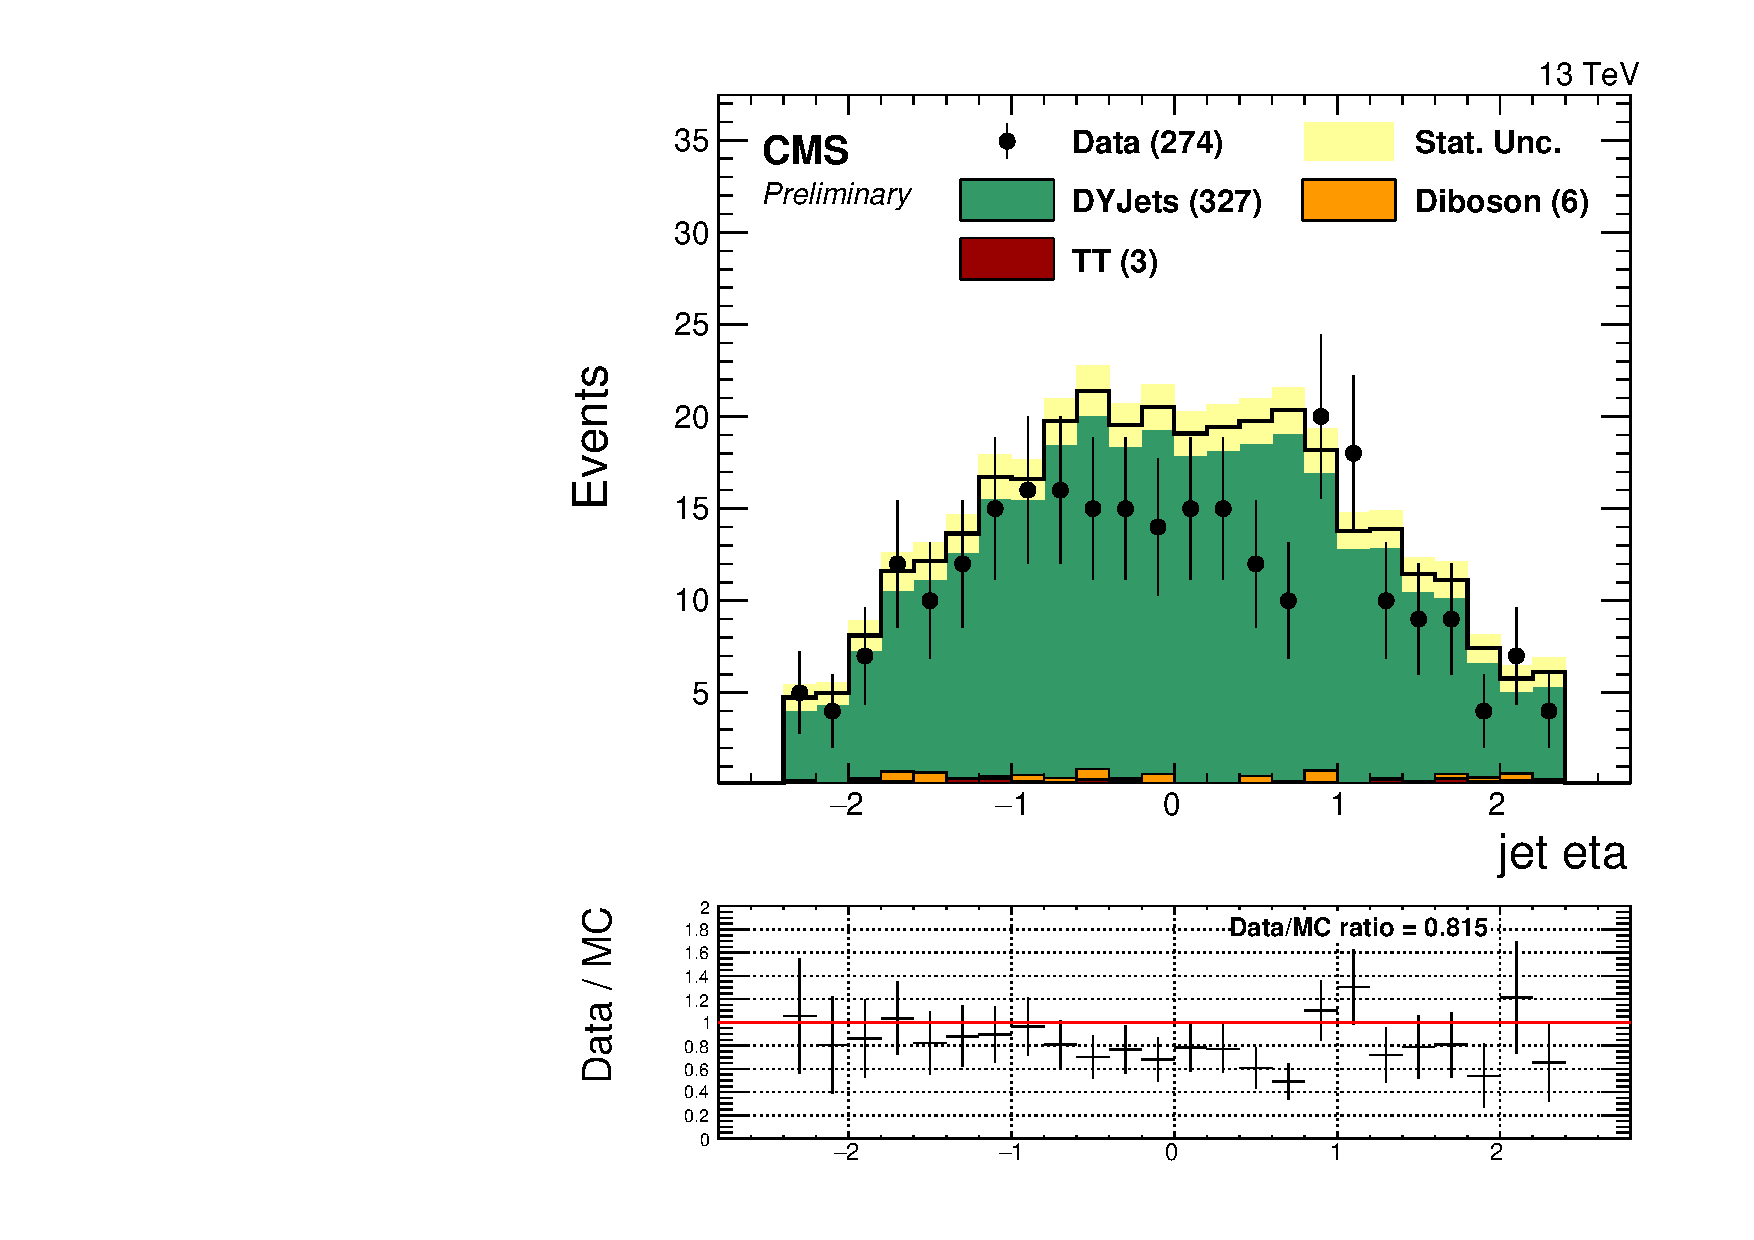
\includegraphics[scale=0.37]{figures/control/etaZjjELP.pdf}\\[2cm]
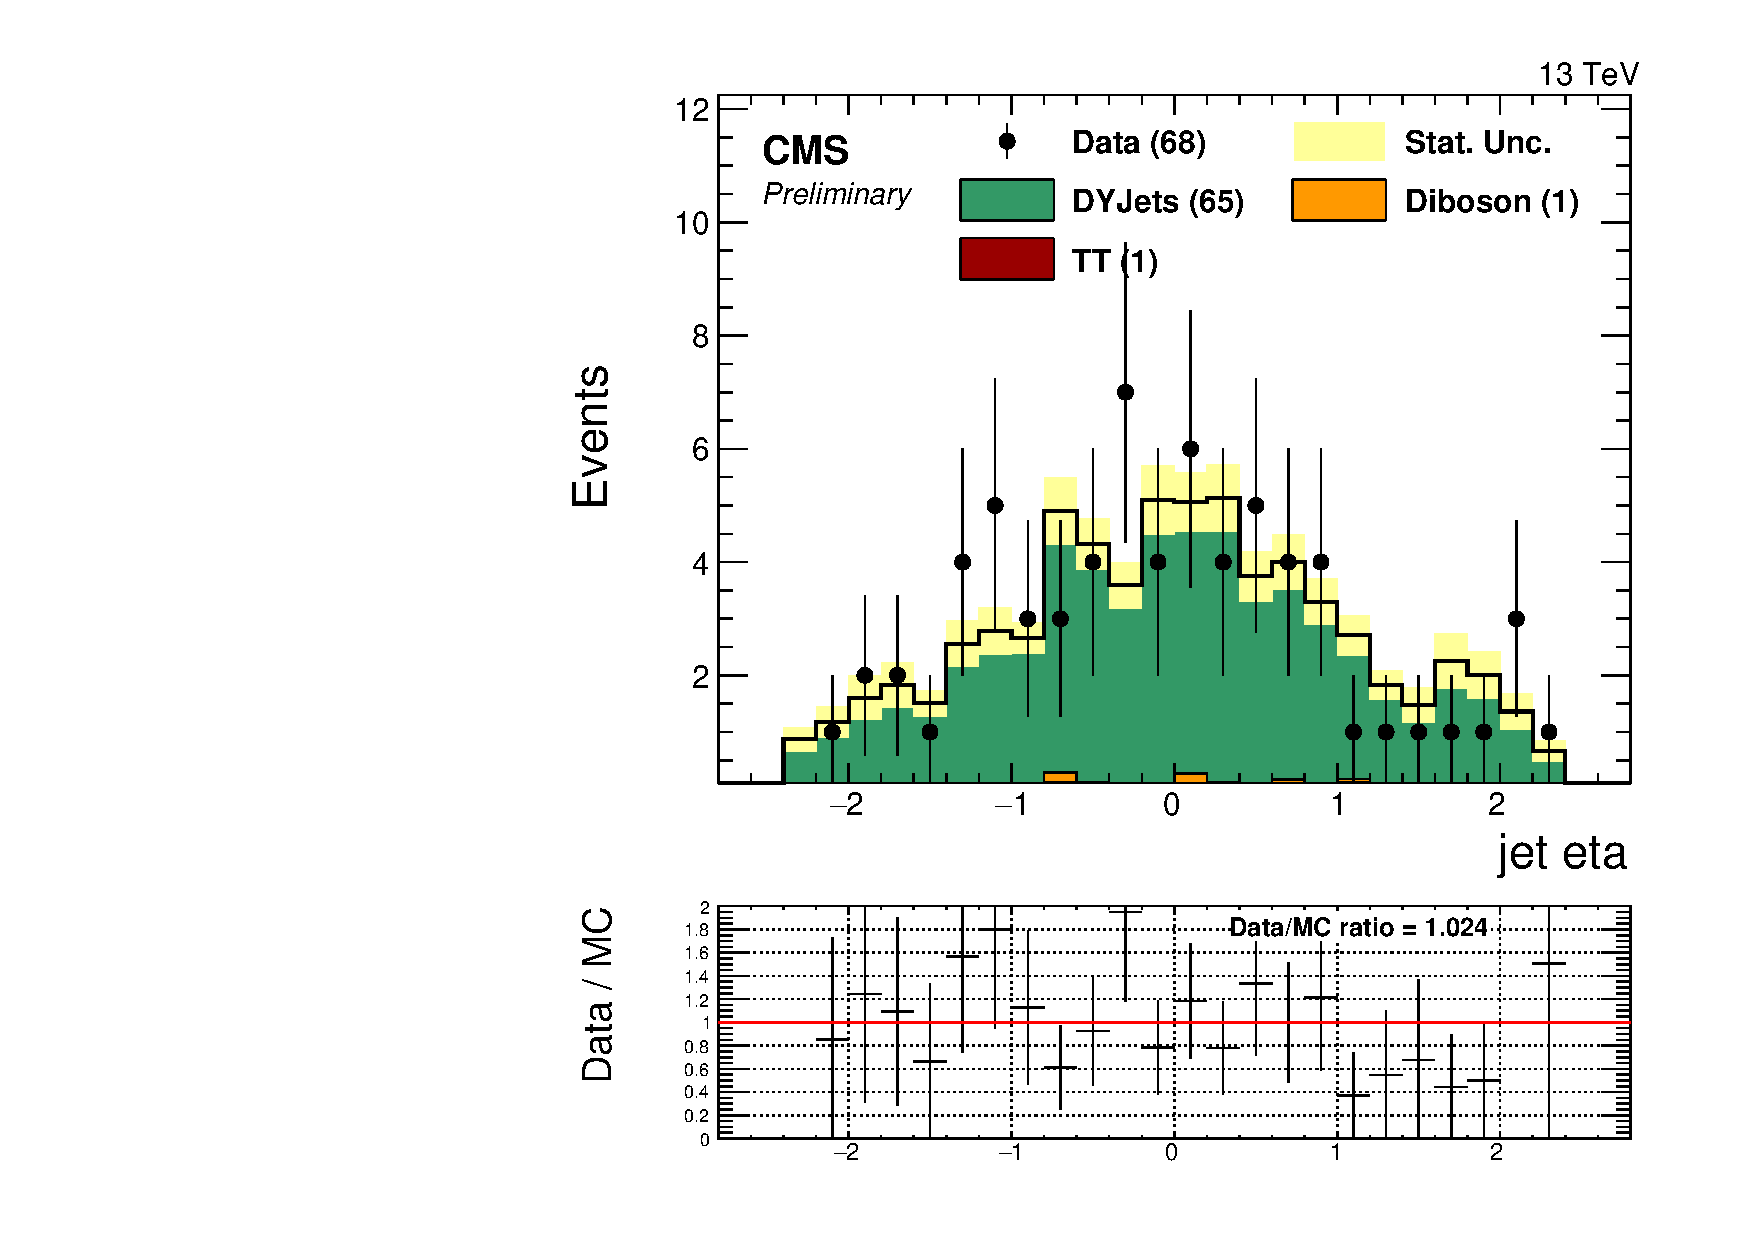
\includegraphics[scale=0.37]{figures/control/etaZjjMHP.pdf}
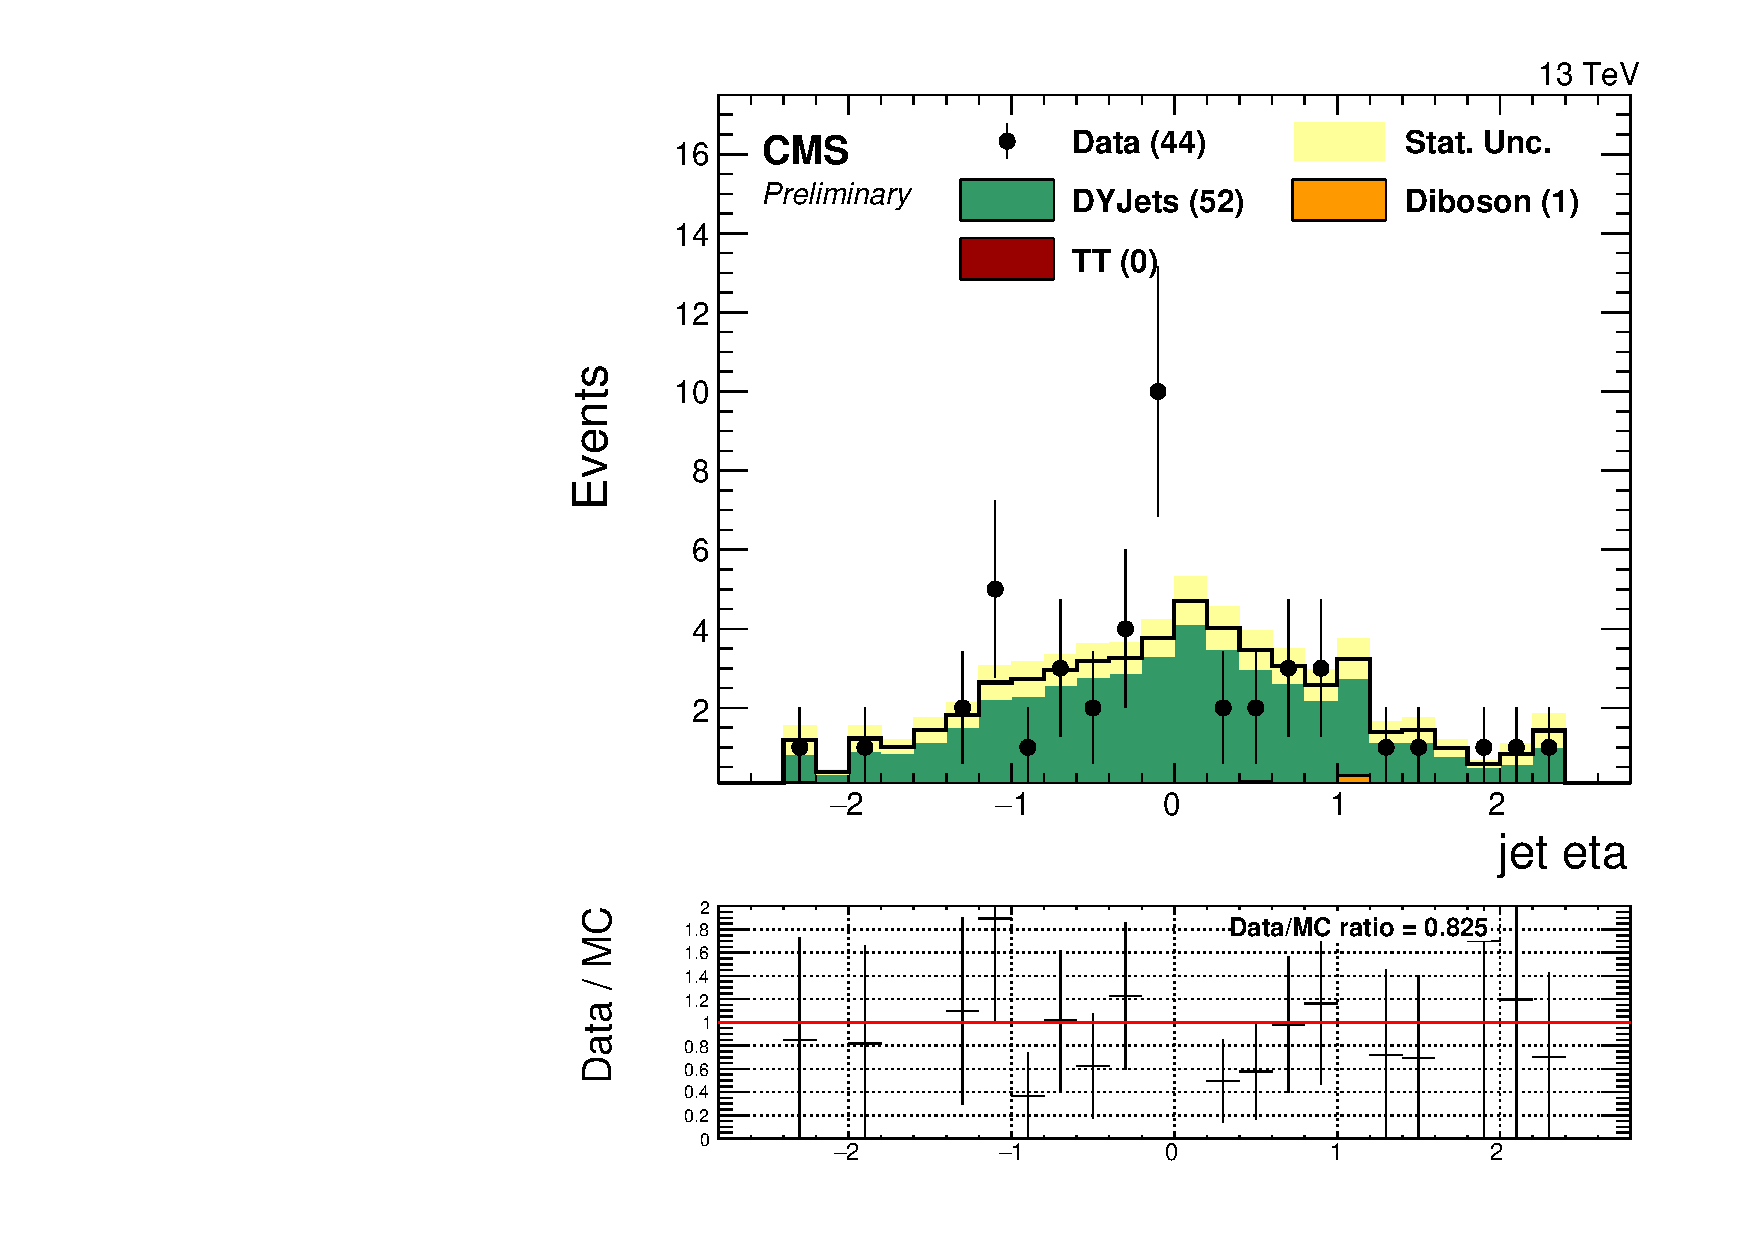
\includegraphics[scale=0.37]{figures/control/etaZjjEHP.pdf}
\caption[Distribution of jet $\eta$]{Distribution of jet $\eta$ in the category: muon low purity (top-left), electron low purity (top-right), muon high purity (bottom-left), and  electron high purity (bottom-right). Simulated backgrounds are displayed as stacked histograms normalized to luminosity (2.7 fb$^{-1}$).}
\label{etaZjj_VZ}
\end{center}
\end{figure}
\begin{figure}[h]
\begin{center}
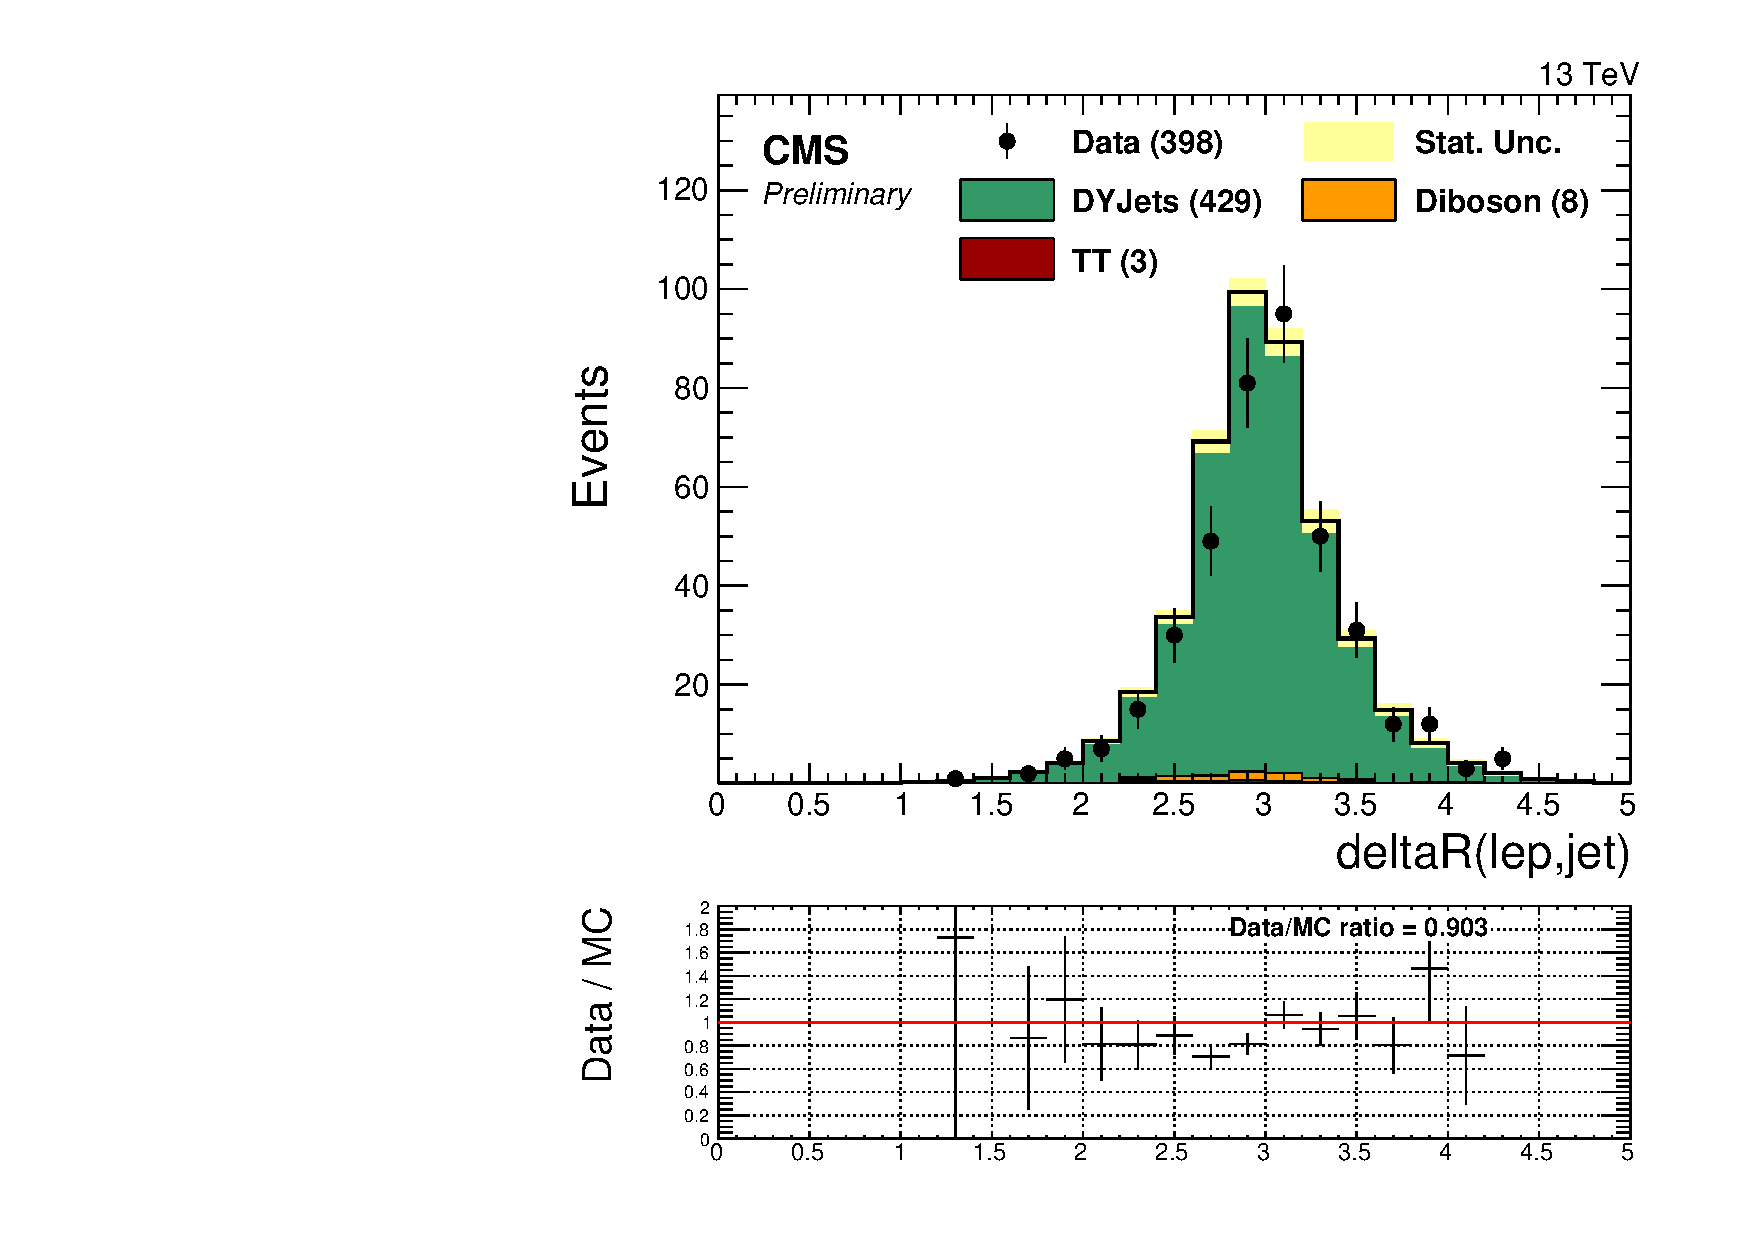
\includegraphics[scale=0.37]{figures/control/deltaRlepjetMLP.pdf}
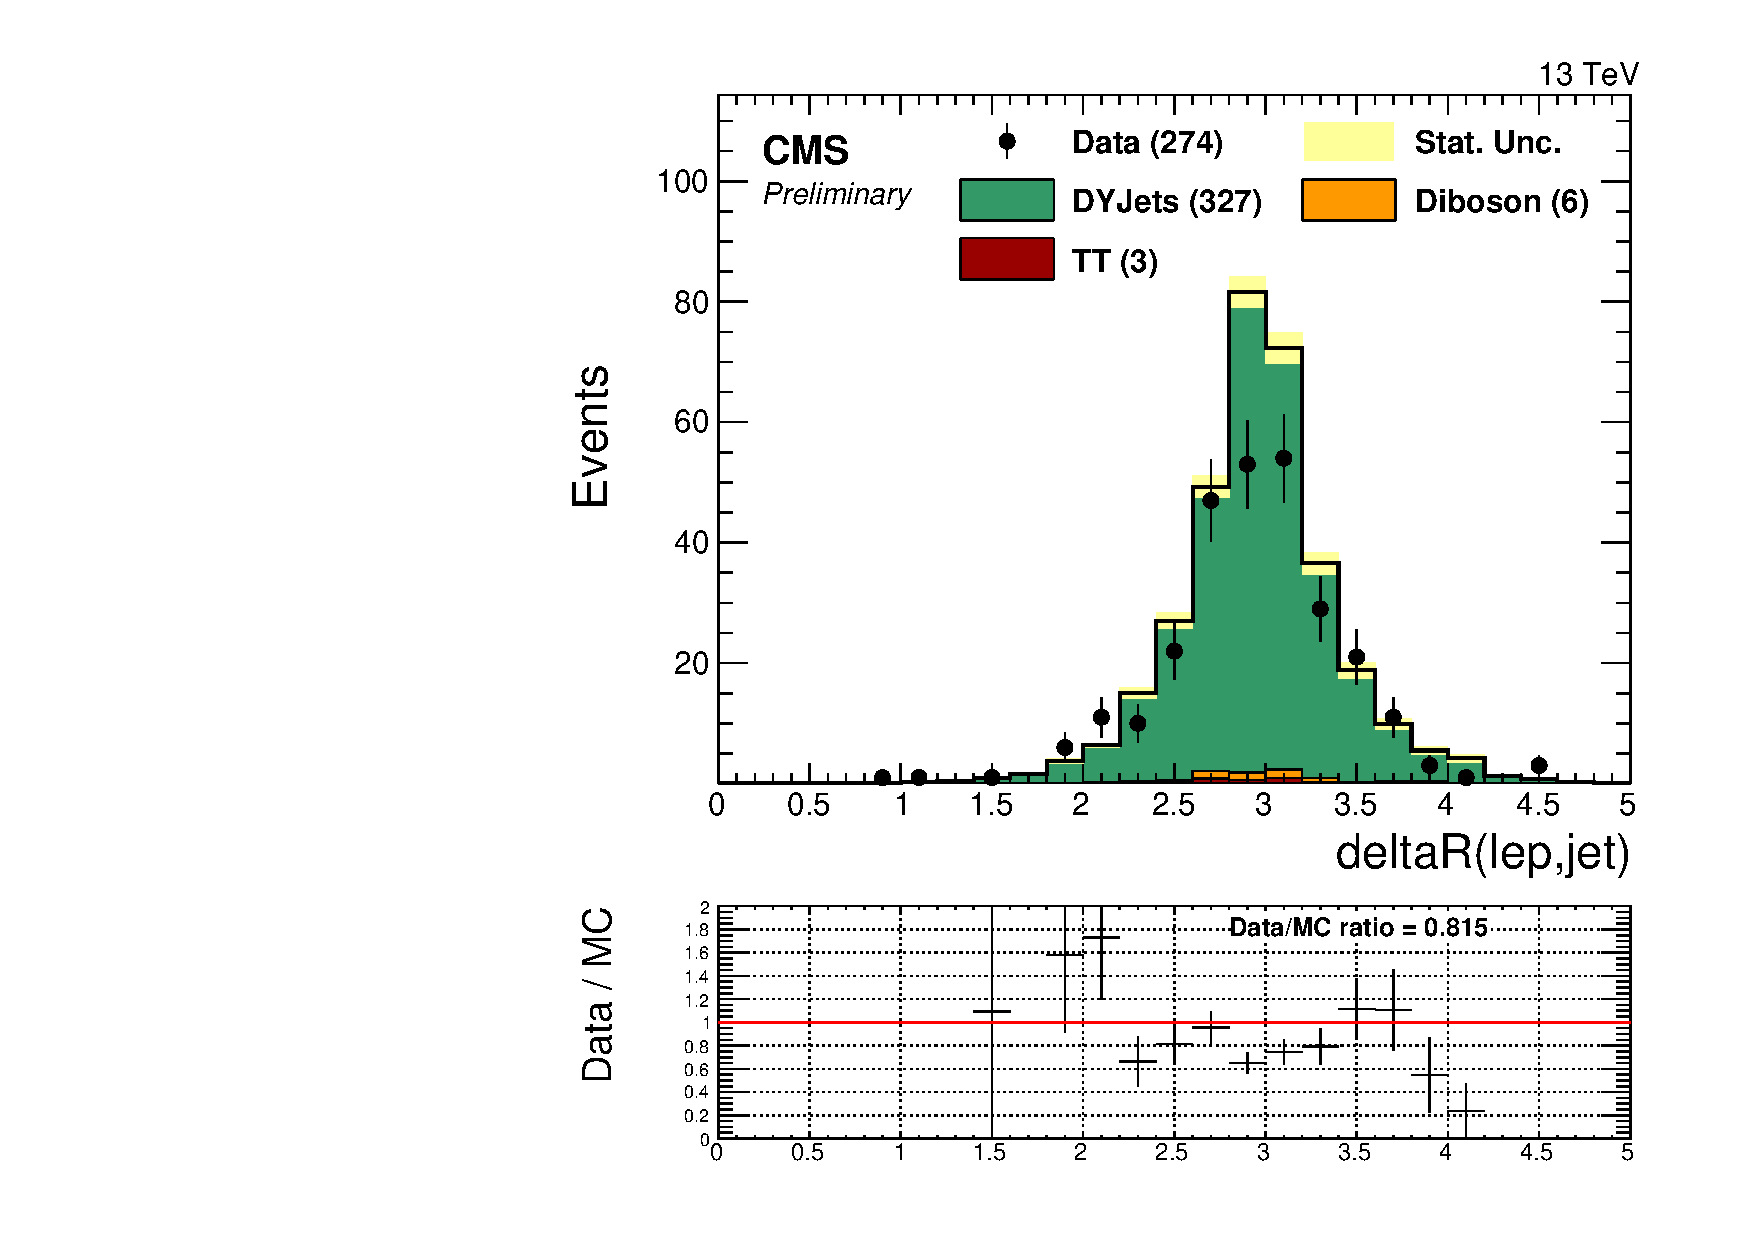
\includegraphics[scale=0.37]{figures/control/deltaRlepjetELP.pdf}\\[2cm]
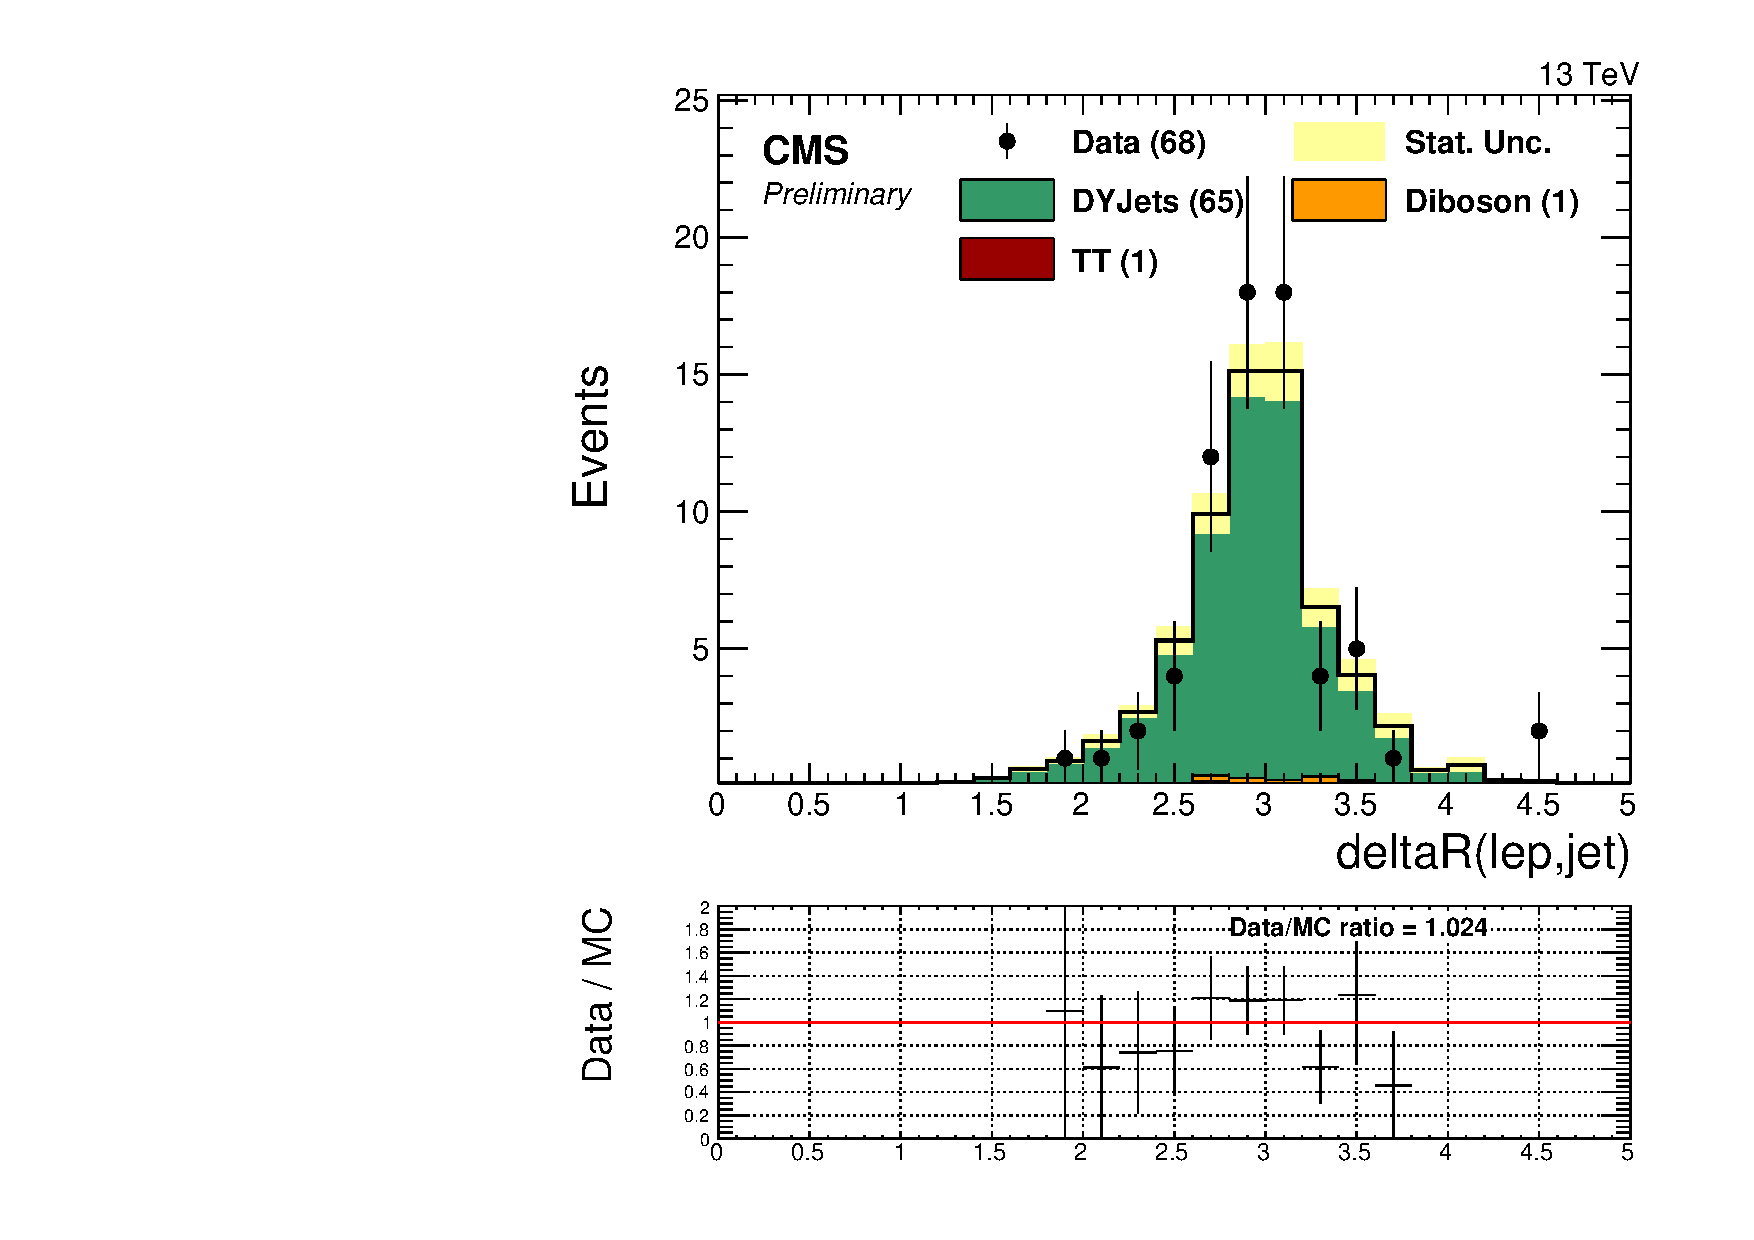
\includegraphics[scale=0.37]{figures/control/deltaRlepjetMHP.pdf}
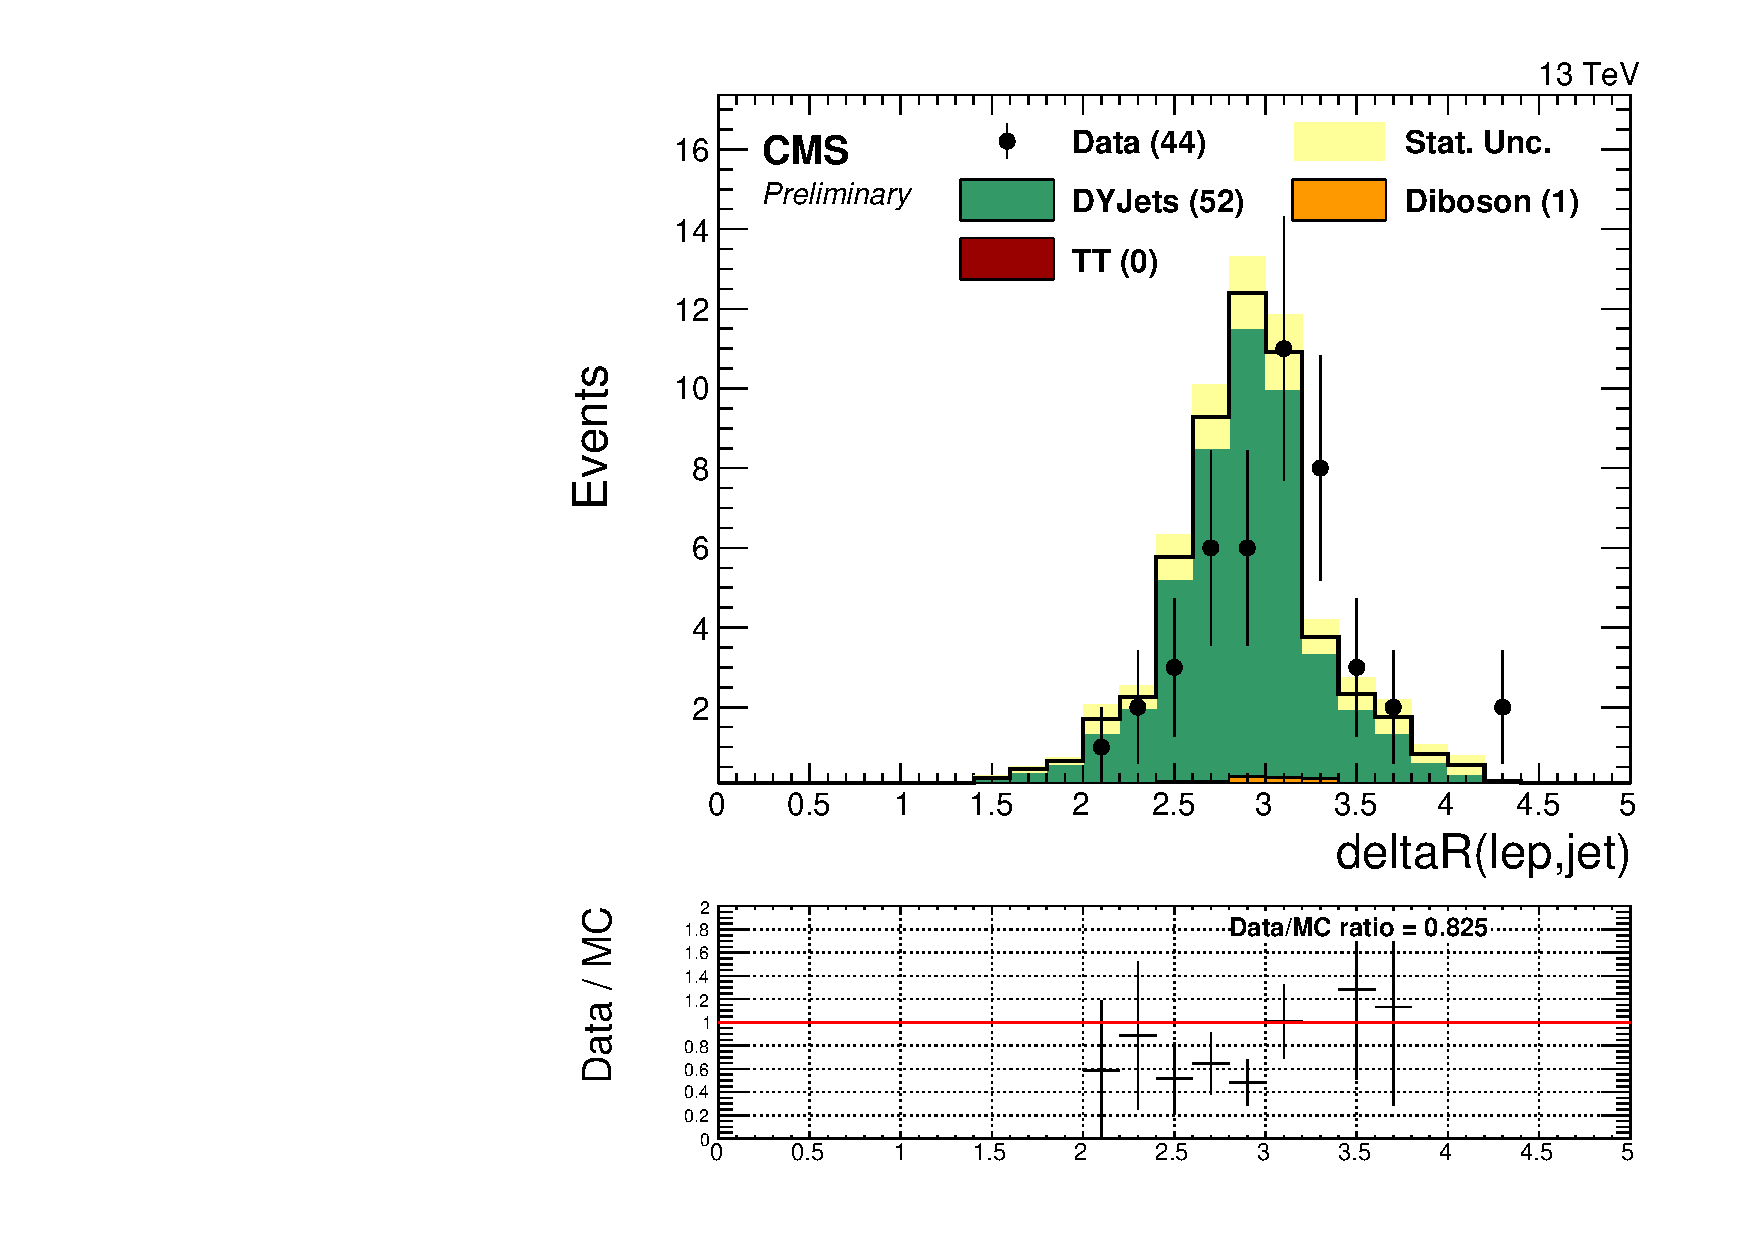
\includegraphics[scale=0.37]{figures/control/deltaRlepjetEHP.pdf}
\caption[Distribution of $\Delta R$ between the jet and the closest lepton]{Distribution of $\Delta R$ between the jet and the closest lepton in the category: muon low purity (top-left), electron low purity (top-right), muon high purity (bottom-left), and  electron high purity (bottom-right). Simulated backgrounds are displayed as stacked histograms normalized to luminosity (2.7 fb$^{-1}$).}
\label{dRlepjet_VZ}
\end{center}
\end{figure}
\begin{figure}[h]
\begin{center}
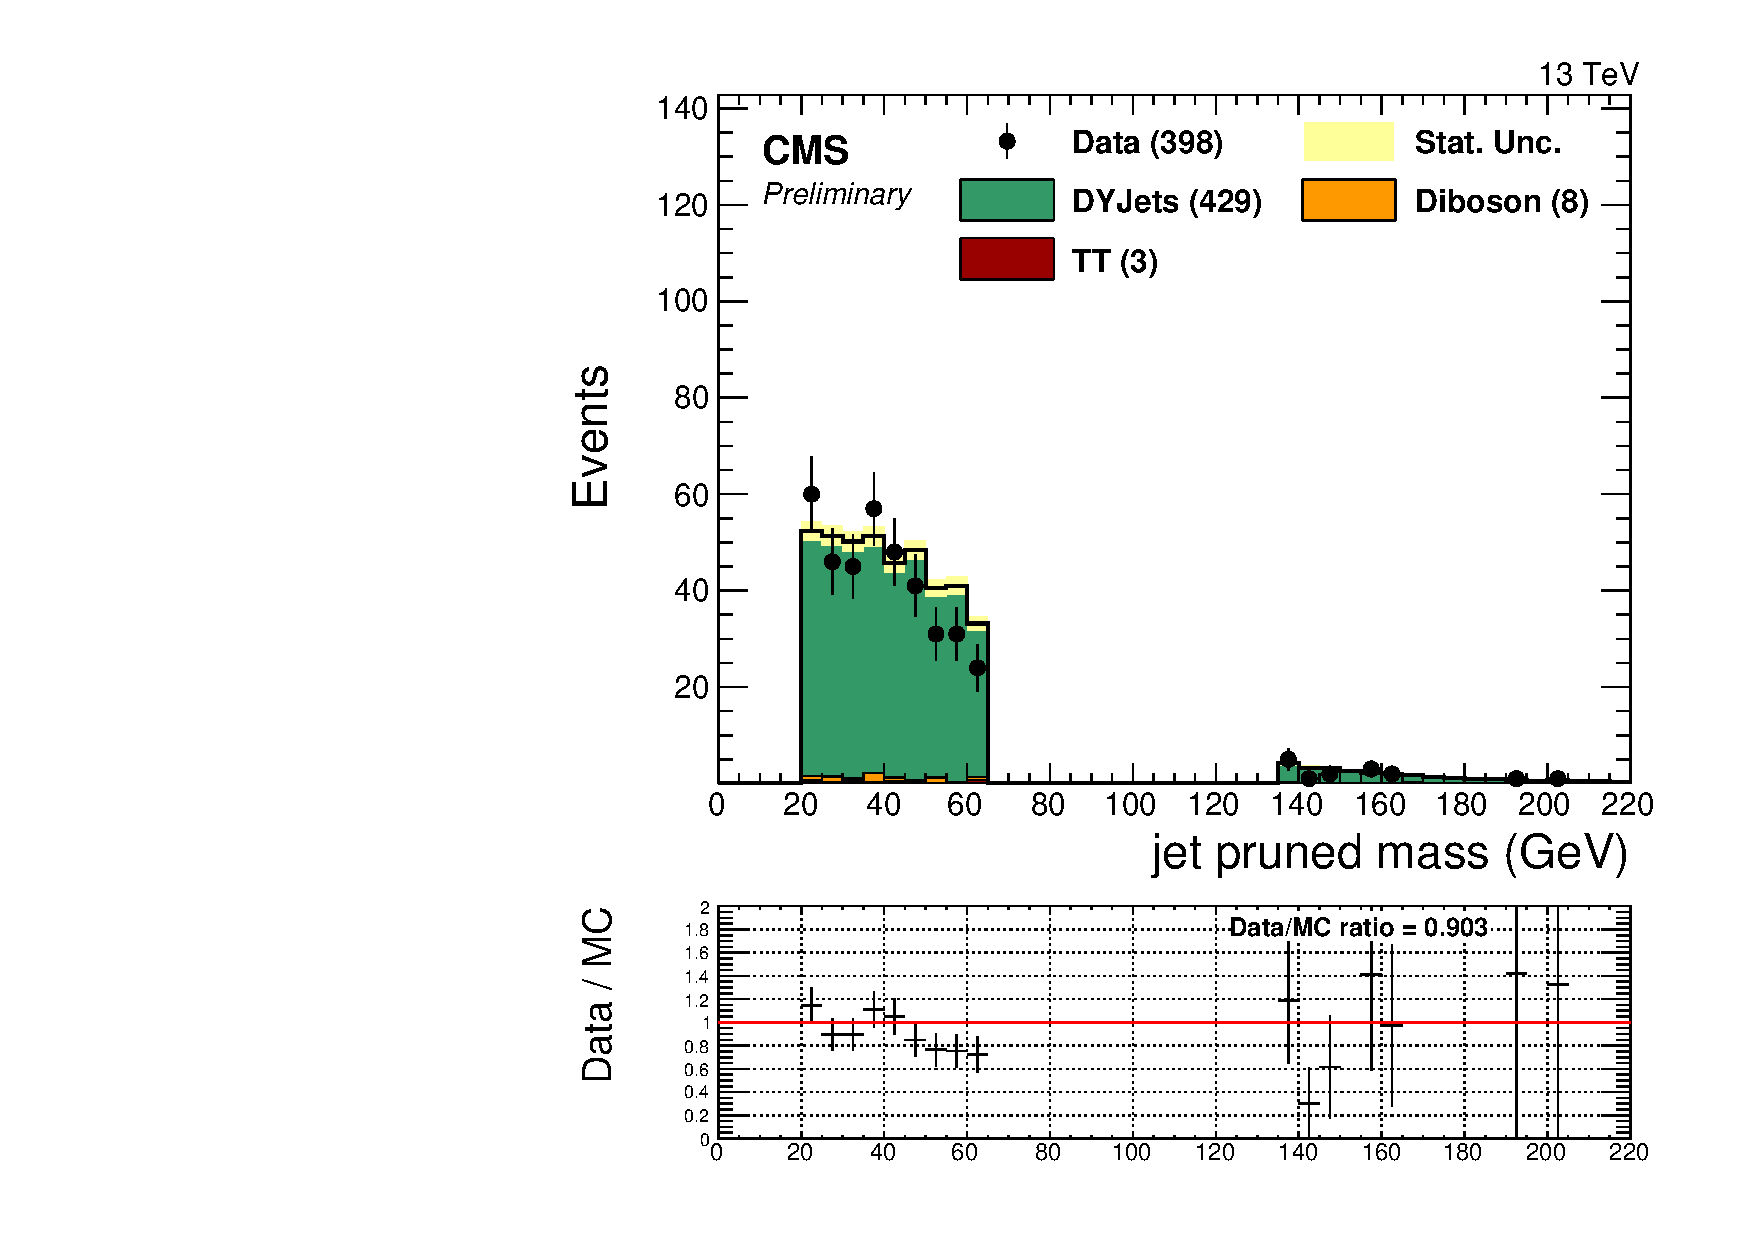
\includegraphics[scale=0.37]{figures/control/massZjjMLP.pdf}
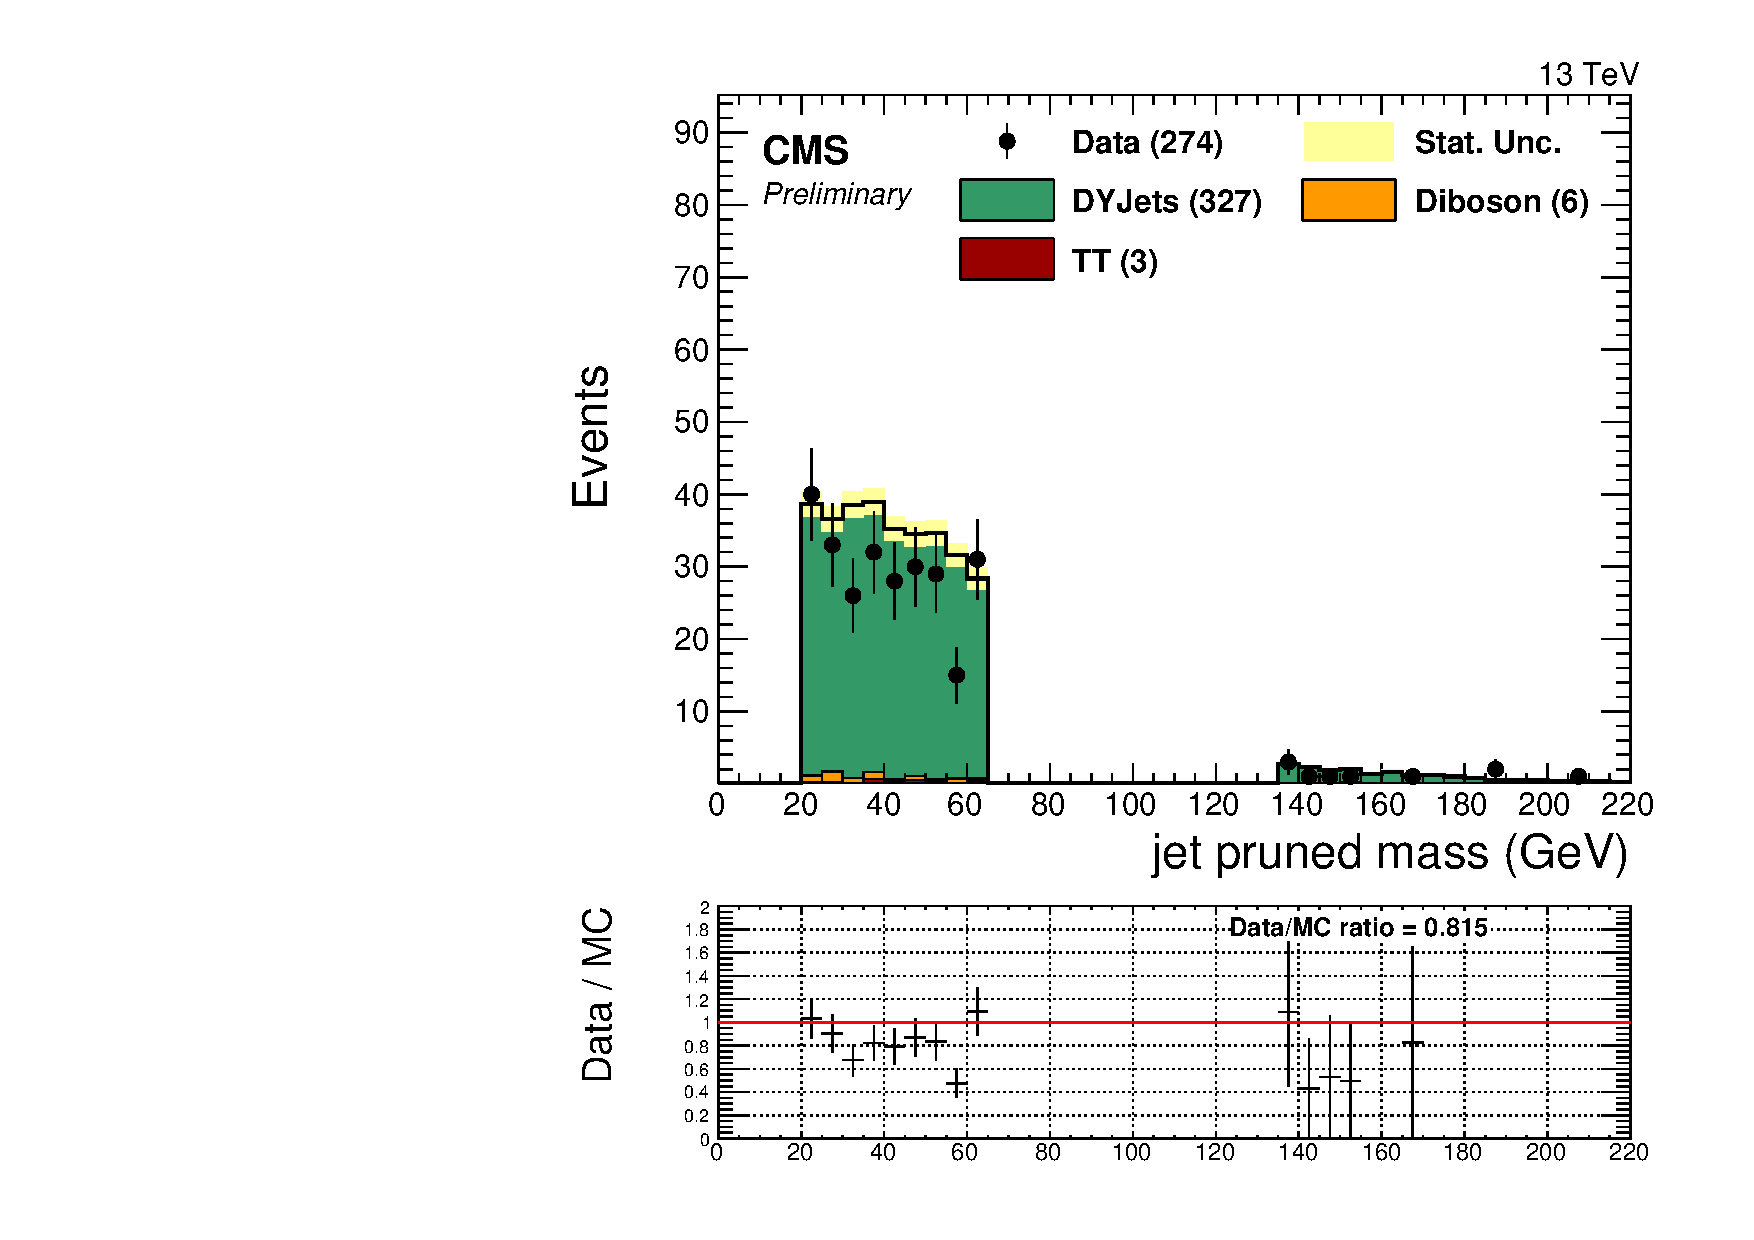
\includegraphics[scale=0.37]{figures/control/massZjjELP.pdf}\\[2cm]
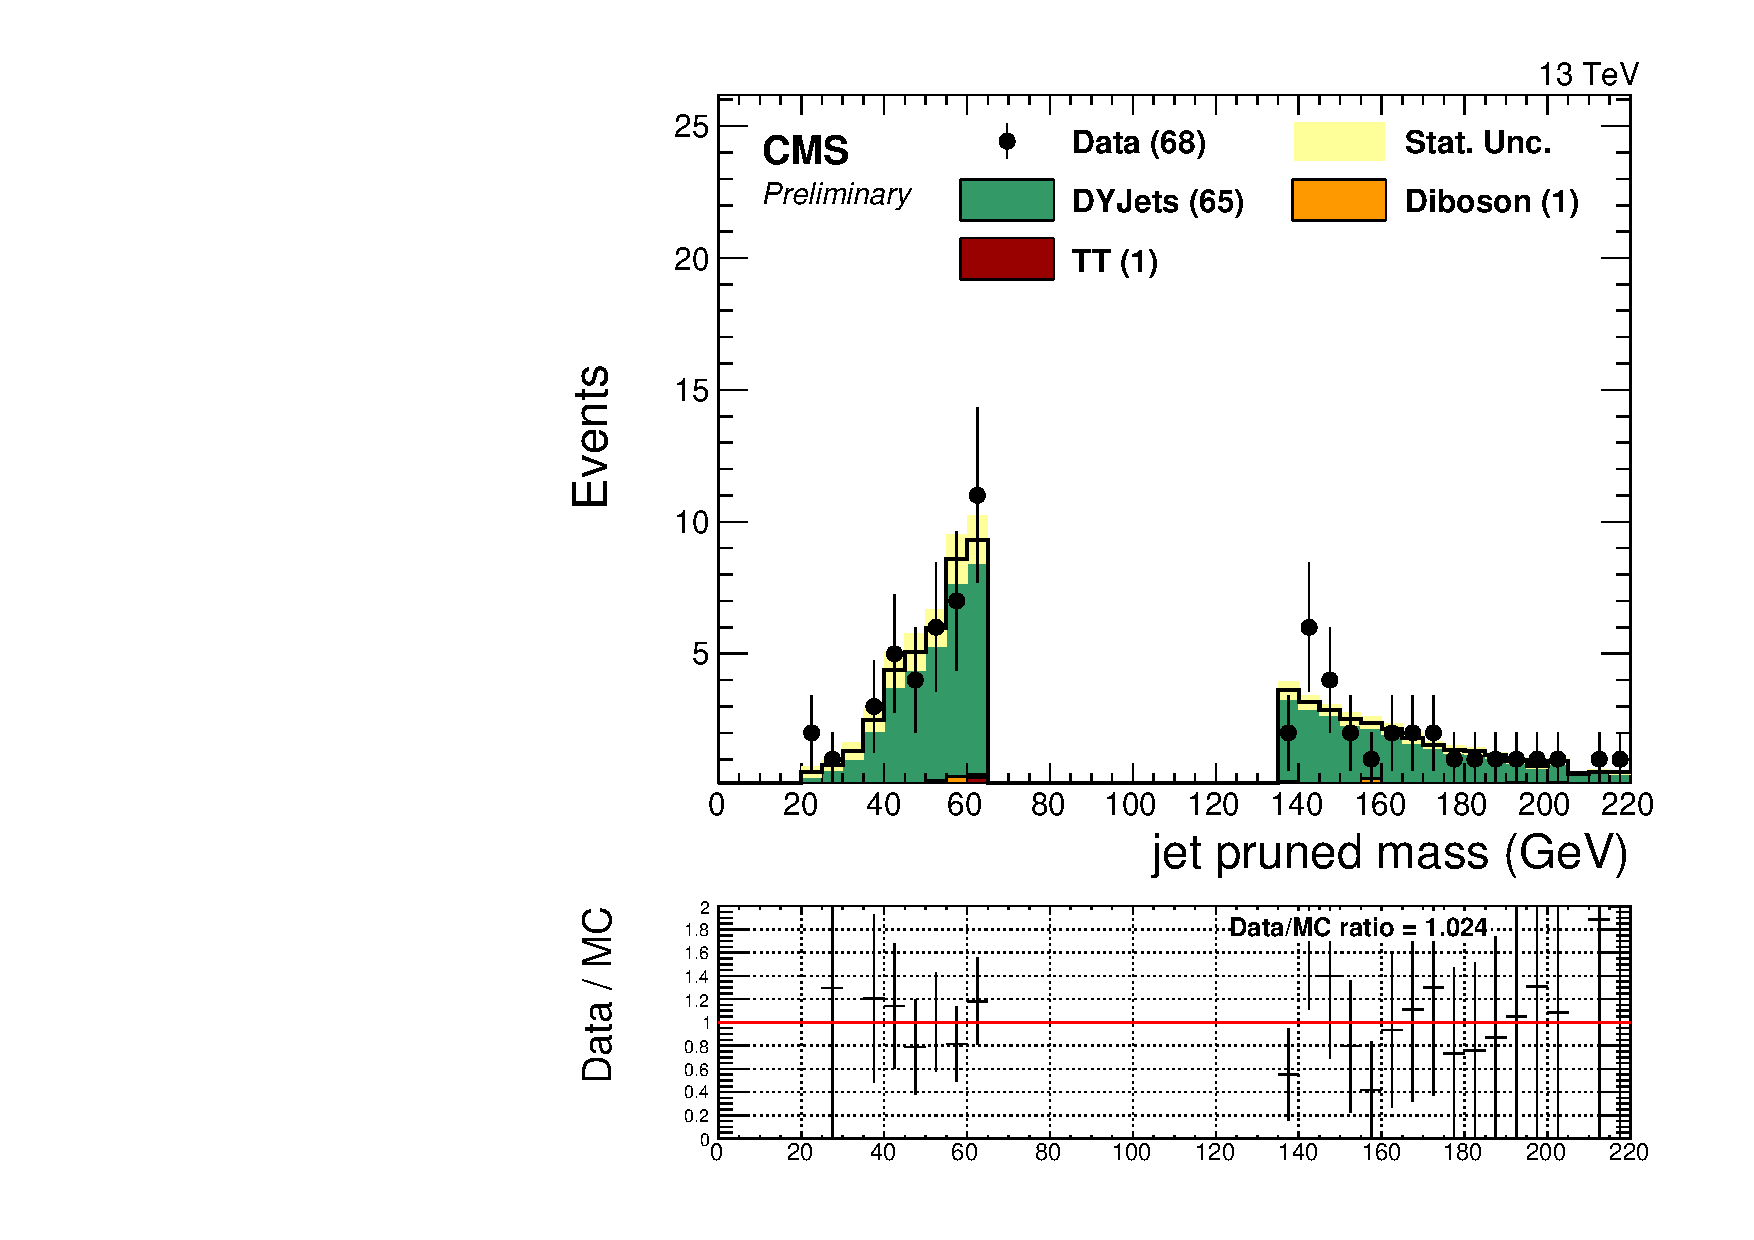
\includegraphics[scale=0.37]{figures/control/massZjjMHP.pdf}
\includegraphics[scale=0.37]{figures/control/massZjjEHP.pdf}
\caption[Distribution of jet pruned mass]{Distribution of jet pruned mass in the category: muon low purity (top-left), electron low purity (top-right), muon high purity (bottom-left), and  electron high purity (bottom-right). Simulated backgrounds are displayed as stacked histograms normalized to luminosity (2.7 fb$^{-1}$).}
\label{massZjj_VZ}
\end{center}
\end{figure}
\begin{figure}[h]
\begin{center}
\includegraphics[scale=0.37]{figures/control/tau21MLP.pdf}
\includegraphics[scale=0.37]{figures/control/tau21ELP.pdf}\\[2cm]
\includegraphics[scale=0.37]{figures/control/tau21MHP.pdf}
\includegraphics[scale=0.37]{figures/control/tau21EHP.pdf}
\caption[Distribution of $\tau_{2}/\tau_{1}=\tau_{21}$]{Distribution of $\tau_{2}/\tau_{1}=\tau_{21}$ in the category: muon low purity (top-left), electron low purity (top-right), muon high purity (bottom-left), and  electron high purity (bottom-right). Simulated backgrounds are displayed as stacked histograms normalized to luminosity (2.7 fb$^{-1}$).}
\label{tau21_VZ}
\end{center}
\end{figure}

\begin{figure}[h]
\begin{center}
\includegraphics[scale=0.37]{figures/control/candMassMLP.pdf}
\includegraphics[scale=0.37]{figures/control/candMassELP.pdf}\\[2cm]
\includegraphics[scale=0.37]{figures/control/candMassMHP.pdf}
\includegraphics[scale=0.37]{figures/control/candMassEHP.pdf}
\caption[Distribution of invariant mass]{Distribution of invariant mass in the category: muon low purity (top-left), electron low purity (top-right), muon high purity (bottom-left), and  electron high purity (bottom-right). Simulated backgrounds are displayed as stacked histograms normalized to luminosity (2.7 fb$^{-1}$).}
\label{fig:candMass_VZ}
\end{center}
\end{figure}

%\clearpage
%\section{Event Displays}
%
%\begin{landscape}
%\begin{figure}[p]
%\centering
%\includegraphics[scale=0.09]{figures/objects/eventDisplay.png}
%\caption[Muon event display]{Event display of a real event observed in the muon channel.}
%\label{fig:muDisplay1}
%\end{figure}
%\end{landscape}
%
%\begin{landscape}
%\begin{figure}[p]
%\centering
%\includegraphics[scale=0.33]{figures/objects/dimuon.png}
%\caption[Muon event display]{Event display of a real event observed in the muon channel.}
%\label{fig:muDisplay2}
%\end{figure}
%\end{landscape}
%
%\begin{landscape}
%\begin{figure}[p]
%\centering
%\includegraphics[scale=0.33]{figures/objects/dielectron.png}
%\caption[Electron event display]{Event display of a real event observed in the electron channel.}
%\label{fig:muDisplay1}
%\end{figure}
%\end{landscape}

